% Supplementary Material of the standard-length version (main_std.tex).
%% Supplementary Material for the manuscript (Mechanical Systems and Signal Processing).
%% Build: latexmk -pdf supplementary.tex   (after main.tex, whose labels it cites via xr)
\documentclass[preprint,12pt]{elsarticle}
\usepackage[T1]{fontenc}
\usepackage{lmodern}
\usepackage{amsmath,amssymb,amsthm}
\usepackage{bm}
\usepackage{graphicx}
\usepackage{booktabs}
\usepackage{multirow}
\usepackage{array}
\usepackage{flafter}
\usepackage{siunitx}
\sisetup{detect-all, range-phrase={--}, range-units=single, per-mode=symbol, group-minimum-digits=5}
\DeclareSIUnit\rpm{rpm}
\usepackage{xr-hyper}
\externaldocument[M-]{main_std}
\usepackage[hidelinks]{hyperref}
\graphicspath{{../}}
\biboptions{numbers,sort&compress}
\newcommand{\sat}{\operatorname{sat}}
\newcommand{\alim}{a_{\lim}}
\newcommand{\achk}{a_{\mathrm{chk}}}
\newcommand{\Vmax}{V_{\max}}
\newcommand{\bmax}{b_{\max}}
\newtheorem{lemma}{Lemma}
\newtheorem{proposition}{Proposition}
\newtheorem{remark}{Remark}
\renewcommand{\thelemma}{S\arabic{lemma}}
\renewcommand{\theproposition}{S\arabic{proposition}}
\renewcommand{\theremark}{S\arabic{remark}}
\renewcommand{\thesection}{S\arabic{section}}
\renewcommand{\thetable}{S\arabic{table}}
\renewcommand{\thefigure}{S\arabic{figure}}
\renewcommand{\theequation}{S\arabic{equation}}
\begin{document}
\begin{frontmatter}
\title{Supplementary Material for ``Beyond linear stability lobes: saturation-induced finite-amplitude instability and basin-aware gain scheduling in actively damped milling''}
\end{frontmatter}
This document collects the proofs, the full text of the passages that the article shortens, and the numerical details, sensitivity checks and secondary results that support the article; Sections~\ref{app:simulator}--\ref{app:software} describe the simulator, the LMI conditions and the software. Section, equation, figure and table numbers without the prefix S refer to the article; in Section~\ref{supp:oz25}, figure numbers without the prefix S are those of \citet{ozsoy2025frequency}.

\section{Supplement to Section 2: model and case study}\label{supp:std-model}

% Material moved from Section 2 of the full version (../sections/s2_model.tex) for the standard-length article.
% Input in Section S1 (supp_model.tex). Text copied verbatim; only references are adapted (M- = main article; no prefix = Supplementary Material).

\subsection{Symbols and terms}\label{supp:std-model-symbols}

Table~\ref{tab:nomenclature} lists the symbols and terms used throughout; the parameters of the case study are in Table~\ref{M-tab:case}.

\begin{table}[!htbp]
  \centering
  \caption{Symbols and terms used throughout; the parameters of the case study are in Table~\ref{M-tab:case}.}
  \label{tab:nomenclature}
  \footnotesize
  \begin{tabular}{@{}>{\raggedright\arraybackslash}p{0.21\textwidth}>{\raggedright\arraybackslash}p{0.58\textwidth}>{\raggedright\arraybackslash}p{0.14\textwidth}@{}}
    \toprule
    Symbol or term & Meaning & Where\\
    \midrule
    $n$; $\Omega$; $T$ & spindle speed in rpm; spindle angular speed; tooth period $2\pi/(N_t\Omega)$ & Eqs.~\eqref{M-eq:phi}--\eqref{M-eq:chip}\\
    $a$; $\alim(g)$ & axial depth of cut; linear (ZOA) stability limit at the gain $g$, $\alim(0)$ without control & Eq.~\eqref{M-eq:char}\\
    $g$; $g_1$, $g_2$, $k_d$ & DVF gain; gains of the delayed law & Eqs.~\eqref{M-eq:dvf}, \eqref{M-eq:comb-law}\\
    Forced orbit $x_p(t)$ & $T$-periodic settled motion below $\alim$, with the clip inactive & Eq.~\eqref{M-eq:xp}\\
    $b(t)$; $\bmax$ & forced command $-g\dot x_p(t)$; its peak, sampled 256 times per tooth period & Eq.~\eqref{M-eq:xp}\\
    $\bar b$; $u_0$ & rigorous upper bound of $\max_t\lvert b(t)\rvert$; free voltage (residual authority) $\Vmax-\bar b$ in the estimates & Sec.~\ref{M-sec:cert-lmi}\\
    Authority & the command range $\lvert V\rvert\le\Vmax$, of which the forced orbit takes $b(t)$ & Sec.~\ref{M-sec:model-orbit}\\
    $\kappa$; $\achk$ & depth margin of the authority condition (0.9); checked depth & Eq.~\eqref{M-eq:achk}\\
    Step entry; face entry; feed ramp & full depth and immersion from $t=0$, starting from rest; tool advancing into a face normal to the feed; feed per tooth rising from zero to $f_z$ over ten revolutions & Sec.~\ref{M-sec:bistab-prot}, \ref{supp:std-bistab-prot}\\
    Kick $\Delta v$; critical kick $\Delta v^*$ & velocity step added to $\dot x$ of the settled cut; the smallest that ends in chatter in the simulator & Sec.~\ref{M-sec:bistab-prot}\\
    Unsafe band & depths below $\alim$ at which some kick of \SI{3}{\milli\metre\per\second} to \SI{3}{\metre\per\second} ends in chatter & Sec.~\ref{M-sec:bistab-prot}\\
    Bistability & coexistence of the forced orbit with a bounded chatter attractor & Sec.~\ref{M-sec:bistab-attr}\\
    D1 & chatter classifier over a window of 300 revolutions & Sec.~\ref{app:simulator}\\
    $\xi$; $E_r$; $k^\top$ & state, regeneration matrix and feedback row of the collocation model ($k$ there is not the modal stiffness) & Eq.~\eqref{M-eq:coll}\\
    $a_{\mathrm{circ}}$ & depth below which the forced orbit of the averaged model attracts every solution & Prop.~\ref{M-prop:circle}\\
    C2; C3 & certificates on the collocation model of the averaged and of the time-periodic model & Sec.~\ref{M-sec:cert-model}\\
    Certified size $\beta$ & along $e=e_2$ the certified kick; along $-\xi_p(0)$, $\beta\ge1$ certifies the step entry & Eq.~\eqref{M-eq:lmi-size}\\
    $\beta_{\mathrm{req}}$; $a_{\mathrm{rob}}$; $a_{\mathrm{cap}}$ & required certified kick; basin-aware depth, up to which every grid depth meets it; assumed depth cap & Eqs.~\eqref{M-eq:admissible}, \eqref{M-eq:arob}\\
    $\tau_s$ & segment length of C3 & Sec.~\ref{app:lmi}\\
    DVF\,+\,D & DVF with the delayed difference term ($k_d=0$) & Eq.~\eqref{M-eq:comb-law}\\
    \bottomrule
  \end{tabular}
\end{table}
% src: src/feasibility.py (KAPPA = 0.9, N_T = 256); src/c1_unsafe_zone.py (N_PHASE = 16, BAND_DV 3 mm/s-3 m/s, ENTRIES: face entry R/f_z = 160 teeth = 40 rev, feed ramp 10 rev); src/tdboundary.py (NREV = 300); src/c2_certificate.py (nodes_for); src/c3_periodic.py (M_C = 16 segments); src/params.py (V_max = F_max/K_a = 9 V)

\subsection{Actuator: units, added damping and limits}\label{supp:std-model-act}

The actuator transfer function $G_a(s)$ of Section~\ref{M-sec:model-loop} is in newtons per volt. While the clip is inactive the loop is linear, with the closed-loop receptance of Eq.~\eqref{M-eq:Gcl}; at $g=\SI{1500}{\volt\second\per\metre}$ the feedback raises the damping of the structural mode from 1.34 to \SI{15}{\percent}.
% src: src/params.py, src/structure.py; verification/zoa_sdm/actuator_mode.json (|Ga|/K_a = 1.004 at 129.3 Hz; structural pole at g = 1500: 15.07 %, against 1.34 % at g = 0)

A proof-mass actuator is limited in three ways: by the voltage or current that its amplifier can supply, by the force that its coil and magnet can produce, and by the stroke of its proof mass. The model contains only the first, as a clip on the command applied before the actuator dynamics. The rated force $F_{\max}=\SI{27}{\newton}$ thus enters only through the voltage $\Vmax=F_{\max}/K_a$ and is not a strict force limit: $\lvert G_a\rvert$ is within \SI{0.4}{\percent} of $K_a$ at the structural mode but peaks at $3.4K_a$ at \SI{8.6}{\hertz}, just above the suspension mode at \SI{8.4}{\hertz}, so transients with low-frequency content can exceed $F_{\max}$; in step entries at $g=1500$ the force reaches \SI{29.5}{\newton}, and a clip at \SI{8.1}{\volt} keeps it at \SI{26.6}{\newton}. The proof-mass stroke needed for a given force falls with the square of the frequency above the suspension mode, so a stroke limit would act mainly on the slow part of an entry transient; neither stroke nor current limits are modelled. The lower clip is compared with the nominal one in Section~\ref{supp:std-delayed-robust}.
% src: src/structure.py (Ga); |Ga|/K_a: 1.0040 at 129.3 Hz, peak 3.371 at 8.60 Hz (recomputed); README §4.6 (clip before the actuator); verification/paper/support_runs.json (clip: peak actuator force 29.52 N at 9 V and 26.63 N at 8.1 V, max_fact of the deepest stable step-entry run at 2500 rpm, g = 1500)

\subsection{Force model: angle convention, surface memory and helix}\label{supp:std-model-force}

The immersion angle $\phi_j$ of Eq.~\eqref{M-eq:phi} is measured clockwise from the feed-normal direction; in half-immersion down milling a tooth cuts while $\phi_j\in[\phi_{\mathrm{st}},\phi_{\mathrm{ex}}]=[\pi/2,\pi]$ (modulo $2\pi$), which is indicated by $\gamma_j(t,z)=1$ ($\gamma_j=0$ otherwise). In the chip thickness of Eq.~\eqref{M-eq:chip}, the surface has been left by the preceding tooth one tooth period $T$ earlier; Section~\ref{app:simulator} replaces $x(t-T)$ by the deepest earlier pass, which matters once the tool leaves the cut. Both $f_s$ and the coefficient $aH(t)$ of Eqs.~\eqref{M-eq:split} and~\eqref{M-eq:aHt} are $T$-periodic. Over one tooth period every axial slice contributes the same mean, only shifted in time by the helix, so the mean coefficient is exactly linear in the depth \citep{altintas1995analytical} [Eq.~\eqref{M-eq:aHmean}], with $\alpha_{yy}$ the directional factor of the feed-normal direction. As the axial tooth pitch $p_a=2\pi R/(N_t\tan\eta)$ is comparable with the depths of interest, the helix keeps $aH(t)$ within about $\pm\SI{12}{\percent}$ of its mean near the stability limit, and $aH$ is constant when $a$ is a multiple of $p_a$ \citep{zatarain2006helix,insperger2006helix}.
% src: src/zoa.py (alpha_matrix), src/tdsim.c (force), src/c3_periodic.py (aH); verification/zoa_sdm/README.md §1 (derivation, alpha_yy = -1.428399); README §12.2 (+-12 % near the limit), §14.4 (pitch 12.57 mm, Table 1)

\subsection{Computation of the linear limit}\label{supp:std-model-zoa}

At a fixed speed, Eq.~\eqref{M-eq:char} gives the depth $a(\omega)$ as a function of the chatter frequency, and $a_{\lim}(g)$ is its smallest real positive value on a scan up to \SI{600}{\hertz} in steps of at most \SI{0.05}{\hertz}, excluding the poles of $a(\omega)$ at the tooth-passing harmonics. It agrees with semi-discretisation of the same averaged model and is conservative by at most about \SI{1}{\percent} with respect to the time-periodic helical model (Section~\ref{app:simulator}).
% src: src/zoa.py (F_GRID: 1200 points over 0.5-60 Hz, i.e. 0.0497 Hz, and 0.02 Hz over 60-600 Hz; pole guard; no root below 60 Hz for g < ~2.4e4 V s/m, verification/zoa_sdm/actuator_mode.json); README §2-3; verification/zoa_sdm/current_grid_check.json (table_96: 1.96e-5); README §3 and Appendix A (time-periodic model: ZOA conservative by 0-1.04 %)

\subsection{Forced orbit: closed form, sampling and dependence on the depth}\label{supp:std-model-orbit}

Below $\alim$ and with the command inside the clip, the deviation decays and the motion converges to a $T$-periodic forced orbit $x_p(t)$. On any $T$-periodic motion the regenerative term of Eq.~\eqref{M-eq:split} vanishes, so $x_p$ is the response of the linear loop \eqref{M-eq:Gcl} to the static force alone, and it has a closed form. Let $\hat f_s(\theta)=\sum_m\hat f_m\,e^{imN_t\theta}$ be the static force per unit depth of the slice at $z=0$, as a function of the spindle angle $\theta=\Omega t$, with $\hat f_m$ its Fourier coefficients over one tooth period. Every other slice carries the same force, delayed in spindle angle by its helix lag $z\tan\eta/R$ [Eq.~\eqref{M-eq:phi}], so the integral over the depth is exact [Eq.~\eqref{M-eq:Fm}]. With $\omega_T=2\pi/T=N_t\Omega$, the orbit and its command are given by Eq.~\eqref{M-eq:xp}, evaluated with $N_h=40$ harmonics. The peak forced command $\bmax=\max_t\lvert b(t)\rvert$ is taken over 256 samples per tooth period; the certificates of Section~\ref{M-sec:certificates} use a rigorous upper bound $\bar b\ge\bmax$ instead (Section~\ref{app:lmi}). The factor in Eq.~\eqref{M-eq:Fm} vanishes when $a$ is a multiple of $p_a/m$, so at a fixed speed the forced command is not monotone in the depth. The orbit persists unchanged in the clipped loop as long as $\bmax<\Vmax$; $b(t)$ is then the command that the actuator supplies in settled cutting, and $\Vmax-\bmax$ is the authority left for any deviation from the orbit.
% src: src/feasibility.py (slice_force_harmonics, force_harmonics, forced_velocity: N_HARM = 40, N_T = 256); README §8.2 (helix cancellation, pitch 12.57 mm); src/c3_periodic.py (closed-form bound with the tail beyond 40 harmonics)

\subsection{Case study: parameters, damping ratio, published cuts and unmodelled effects}\label{supp:std-model-case}

Table~\ref{M-tab:case} lists the parameters, all taken from \citet{ozsoy2026robust} except those marked as derived or chosen here, and Table~\ref{tab:nomenclature} the symbols and terms used throughout. The flexible direction, not stated in the text of \citet{ozsoy2026robust}, is taken normal to the feed, along the actuator axis; this reproduces their uncontrolled stability chart with a median deviation of \SI{0.04}{\percent} over \SIrange{400}{3000}{\rpm}. The damping ratio is \SI{1.34}{\percent} rather than the \SI{1.45}{\percent} of their Table~1, because the receptance, pole and stability chart computed in that paper are fitted by the former, and Table~2 of \citet{ozsoy2025frequency} gives \SI{1.34}{\percent} for the same structure; with \SI{1.45}{\percent} the uncontrolled chart deviates by \SI{8}{\percent} (median), whereas the gain map of Section~\ref{M-sec:feas-pub} changes by a median factor of 1.00.
% src: README §2, §4.1, §5.1, §6; verification/consistency/a_damping.json (fig6a peak -111.10 dB, model -111.10 dB at 1.34 % and -111.79 dB at 1.45 %; fig6b pole 1.3405 %; fig9 fit 1.3394 %); results/paper_vs_ours.json (p05: 0.037 % at 1.34 %, 7.99 % at 1.45 %); results/gainmap_zeta145.npz vs gainmap_main.npz (median gain ratio 0.995)

The model was checked against the cutting tests of \citet{ozsoy2026robust}, and against a second data set on the same set-up in Section~\ref{M-sec:model-second}. At the gains used in the tests, the linear limit classifies 17 of the 19 distinct published cuts as measured. The two exceptions are controlled cuts that chattered below the predicted limit, at \SI{1300}{\rpm} and \SI{10}{\milli\metre} ($0.80\alim$) and at \SI{2800}{\rpm} and \SI{5.5}{\milli\metre} ($0.76\alim$); at the first, the frequency at which the model loses stability, \SI{149.0}{\hertz}, is close to the strongest measured peak, \SI{149.5}{\hertz}. The clipped model does not make them chatter either: their forced commands at the published gains, 3.5 and \SI{3.0}{\volt}, leave more than \SI{5}{\volt} free, step and face entries settle at both, and the critical kick is 25--\SI{27}{\milli\metre\per\second} over 16 kick phases at \SI{1300}{\rpm} (23--\SI{24}{\percent} of the cutting impulse of one tooth period), whereas no kick up to \SI{3}{\metre\per\second} causes chatter at \SI{2800}{\rpm}. Saturation-induced finite-amplitude instability (Section~\ref{M-sec:bistability}) thus cannot explain the second cut, and explains the first only if the test contained a perturbation of that size, which neither simulated entry produces; otherwise the model overestimates the controlled limit there by at least 25 and \SI{32}{\percent}.
Where chatter frequencies can be compared, model and measurement differ by 0.5--\SI{4}{\hertz}. The measured spectra also contain spindle harmonics that are not multiples of the tooth-passing frequency (the seventh is the strongest peak of the stable cut at \SI{1300}{\rpm} and \SI{8}{\milli\metre}), a sign of runout \citep{insperger2008chatter}, which the model omits. Like \citet{ozsoy2026robust}, the model neglects the beam modes of the set-up at 23 and \SI{47}{\hertz}, and it uses the exact velocity, which they estimate by integration and zero-phase filtering. The flute length and overhang of the tool, the mode shape over the depth, the proof mass and its stroke, the sensor and the loop latency are not reported in \citet{ozsoy2026robust} and are not modelled: the tool is rigid, the mode uniform over the depth and the loop, outside Sections~\ref{M-sec:ba-valid} and~\ref{M-sec:delayed}, without delay. The depths and kicks reported below are predictions of this model.
% src: results/cuts_main.json (21 marks, 19 distinct cuts; pred_paper equals measured at 17/19; 1300 rpm, 10 mm: g_paper 1157.98 V s/m, alim_paper 12.478 mm (10/12.478 = 0.80), fc_paper 149.03 Hz; 2800 rpm, 5.5 mm: g_paper 679.55 V s/m, alim_paper 7.264 mm (5.5/7.264 = 0.76)); verification/targets/fft_peaks.csv (Fig10 B: tallest peak 149.5 Hz; Fig10 A: tallest peak 151.6 Hz, spindle harmonic 7); README §5.6 (12B 131.9 vs 133.3 Hz, 12D 134.0 vs 138.1 Hz; 10B 149.0 vs 149.5 Hz), §4.6 (velocity estimated by integration and zero-phase filtering in the demand check of the base paper), §7 (beam modes 23 and 47 Hz neglected as in the base paper); verification/targets/targets.md (Table 1 of the base paper: beam modes 23 and 47 Hz; no flute length, overhang, mode shape, proof mass, stroke, sensor, sampling rate or latency recorded)
% src: verification/paper/revision_runs.json (closed_form.published_cuts: bmax_V 3.525 at 1300 rpm/10 mm, g 1157.98, and 3.000 at 2800 rpm/5.5 mm, g 679.55, i.e. 9 - bmax = 5.47 and 6.00 V; tooth_impulse_Ns 2.234, mass 20.30 kg; published_cuts_entries: step and face entries, 9 V clip, full surface memory (NREG = 0), chatter false at both cuts; published_cuts_kicks_mps: 1300 rpm 0.02505-0.02673 m/s over 16 phases, 2800 rpm inf at all 16 phases, i.e. no kick of DV_GRID up to DV_HI = 3 m/s (src/c1_unsafe_zone.py); impulse ratio 0.02505 x 20.30 / 2.234 = 0.228 to 0.02673 x 20.30 / 2.234 = 0.243; overestimate 12.478/10 = 1.248 and 7.264/5.5 = 1.321)

\subsection{The second data set: full statement of the comparison}\label{supp:std-model-second}

\citet{ozsoy2025frequency} report further tests on the same set-up; their Table~2, Eq.~(2) and Section~3.2 give the structure, actuator, tool and cutting constants of Table~\ref{M-tab:case}, including the damping ratio of \SI{1.34}{\percent} inferred above. Two groups of their tests were digitised, each twice and independently, with identical readings (Section~\ref{supp:oz25-data}): 39 controlled cuts with DVF at $g=\SI{253}{\volt\second\per\metre}$ reported stable, marginal or chattering (their Fig.~6), and 56 tests at 1700--\SI{2200}{\rpm} made after the workpiece had been clamped again (\SI{128.1}{\hertz}, \SI{1.48}{\percent}, \SI{1.13e7}{\newton\per\metre}), with the measured amplitude of the command or the mark that the actuator saturated (their Figs.~10 and 12). They form a second data set on the same rig, not a second machine.

The linear model reproduces their uncontrolled and controlled stability charts to 0.04 and \SI{0.14}{\milli\metre} (RMS, outside the steep flanks of the lobes) for the first structure and to 0.06 and \SI{0.07}{\milli\metre} for the second, whose gain, not stated, a fit of the chart puts at \SI{251}{\volt\second\per\metre}, within \SI{1}{\percent} of the \SI{253}{\volt\second\per\metre} of the first group, which is used below. Of the 39 controlled cuts, the model and their chart classify the same 26 as measured. Nine of the others are stable cuts at 700--\SI{1100}{\rpm} above the predicted limit, where the cutting speed is only 0.6--\SI{0.9}{\metre\per\second} and process damping, which the model omits, may raise the limit; two are stable cuts at 2800 and \SI{2900}{\rpm}, and two, marginal and chattering at \SI{2100}{\rpm}, lie below the limit.
% src: verification/ozsoy2025/setup2025.py (Table 2 of the 2025 article = src/params.py; RECLAMPED 128.1 Hz, 1.48 %, 1.13e7 N/m), digitise_notes.md, points_fig6.json, points_fig10.json; verification/ozsoy2025/fit_gain.py/.json (fig6: uncontrolled rms 0.040 mm, controlled_g253 rms 0.137 mm; fig10_uncontrolled rms 0.062 mm; fig10_gain_fit g_best 251, rms_at_253 0.074 mm); compare2025.py/.json and a recomputation with the digitised controlled curve of Fig. 6 (26 of 39 classified as measured by both, the same 13 mismatches: stable at 700 (4, 5, 7 mm), 800 (5), 900 (10, 12), 1000 (12, 15), 1100 (4), 2800 (4), 2900 (5); marginal 2100/5 and chatter 2100/6); cutting speed pi D n: 0.59 m/s at 700 rpm, 0.92 m/s at 1100 rpm

For the 36 unsaturated tests of the second group, the settled forced demand $K_ag\max\lvert\dot x_p\rvert$ (Section~\ref{M-sec:model-orbit}; \SI{27}{\newton} corresponds to the \SI{9}{\volt} clip) is 0.90 times the measured amplitude (median; interquartile range 0.83--1.02), and within \SI{2.5}{\newton} of it (median \SI{0.85}{\newton}) at the 16 tests of up to \SI{5}{\milli\metre} at 1700--\SI{2000}{\rpm} (Fig.~\ref{M-fig:oz25}b). At \SI{15}{\milli\metre} it is about twice the measured value: like the frequency-domain prediction of \citet{ozsoy2025frequency}, the model misses the measured minimum of the command near \SI{15}{\milli\metre}, while the force of a \SI{45}{\degree} helix is most nearly constant at the axial pitch, \SI{12.6}{\milli\metre}; an effective helix of \SI{42}{\degree} would remove much of this error, which points to the axial distribution of the force or of the mode (Section~\ref{supp:oz25-sat}). At 2050--\SI{2200}{\rpm} the measured command at 2--\SI{3}{\milli\metre} is 1.1 to 2.3 times the prediction. The settled cut is predicted to saturate at 4 of the 20 saturated tests; the command reaches the clip during the simulated face entry at 12 of them, and later at two more, through simulated chatter above the controlled limit.
% src: verification/ozsoy2025/forced_map.py (demand_components), sim2025.py/.json, compare2025.py/.json (fig10.amplitude_peak: n 36, median_ratio_pred_over_meas 0.903, ratio_q25_q75 0.832-1.021; abs_error_depth_le5_rpm_le2000_N: n 16, median 0.85, max 2.46; demand_over_measured.depth_15: median 2.05 (1.23-2.64); measured over predicted at 2050-2200 rpm, 2-3 mm: 1.09-2.34 (recomputed from rows); saturation_settled_closed_form both 4 of 20; saturation_any_time_face_entry both 14, pred_only 2); helix2025.py/.json (mean_abs_log 0.240 at 45 deg, 0.159 at 42 deg; pitch 12.57 mm at 45 deg)

Relative to the linear limits of the model (Fig.~\ref{M-fig:oz25}a), the measured outcomes fall as follows. All 37 tests below the uncontrolled limit settled, 10 of them saturated. Between the uncontrolled and the controlled limit, 5 of the 7 saturated tests chattered or were marginal, and none of the 6 unsaturated ones did (one-sided Fisher exact test, $p=0.016$; for chatter alone, 2 of 7 against 0 of 6, $p=0.27$); above the controlled limit the 3 saturated tests chattered, while 3 unsaturated ones at 1700--\SI{1800}{\rpm} and 20--\SI{22}{\milli\metre}, above the model's and the published controlled limit, were stable. The model does not reproduce the 5 losses of stability between the limits: it predicts their settled command at 12--\SI{19}{\newton}, except at \SI{1950}{\rpm} and \SI{20}{\milli\metre} (\SI{33}{\newton}), both simulated entries settle, and, with kicks at four phases, a kick of at most \SI{3}{\metre\per\second} ends in chatter at only two of the five tests, both marginal, with critical kicks of 0.14 and \SI{0.40}{\metre\per\second}, whose impulses $m\Delta v^*$, with the modal mass of the re-clamped structure ($k/\omega_n^2=\SI{17.4}{\kilogram}$), are 1.7 and 2.3 times the cutting impulse of one tooth period [Eq.~\eqref{M-eq:impulse}]; at the other three, among them the chatter tests at 2050 and \SI{2100}{\rpm}, no kick up to \SI{3}{\metre\per\second} at these phases makes the model chatter. There the measured command exceeds the prediction, as noted, and \citet{ozsoy2025frequency} report disagreement with their own frequency-domain model at 2050--\SI{2200}{\rpm}, which they relate to loss of contact of the actuator or other nonlinearities; for the first structure, their time-domain simulation, whose details are not given, places the onset of saturation at \SI{2100}{\rpm} at \SI{4.5}{\milli\metre} (their Fig.~6), where the forced demand of the present model is \SI{13.5}{\newton} (\SI{14.2}{\newton} for the re-clamped structure). The saturation tests are thus consistent with the mechanism of this paper: below the controlled limit, losses of stability occurred only above the uncontrolled limit and only in tests whose command saturated. As a cut that chatters also drives the command into the clip, and the article does not say when during a test the command saturated, the data cannot show that the saturation came first. They support the forced demand at depths of up to \SI{5}{\milli\metre} at 1700--\SI{2000}{\rpm}, but the model does not predict these losses of stability.
% src: verification/ozsoy2025/compare2025.json (fig10.by_position: below a_lim(0) n 37, sat 10, unstable 0; between n 13; above a_lim(g) n 6, chatter 3, sat 3; between_sat_vs_outcome 5/2 against 0/6, fisher_one_sided_p 0.0163; rows: 1700/20, 1750/20, 1800/22 stable above a_lim(g)); kicks2025.py/.json (13 points between the limits: finite at 2000/10 (138.7 mm/s, marginal) and 1950/20 (396.5 mm/s, marginal), inf at the other 11); onset2025.py/.json (first structure, squares of the article's Fig. 6; 2100 rpm: article onset 4.5 mm, demand there 13.5 N, no model onset below a_lim(g) = 7.78 mm); re-clamped structure at 2100 rpm / 4.5 mm: forced_demand 14.15 N (feasibility.forced_demand after setup2025.apply_structure(RECLAMPED)); article Sec. 4.2 (disparity at 2050-2200 rpm, 'actuator loss of contact effects or other nonlinearities'); kicks at phases 0, 4, 8, 12 of 16 (kicks2025.py PHASES; crit_by_phase_mmps finite at all four phases at 1950/20 and 2000/10, none at 2050/5, 2100/5, 2150/5); impulse ratio m dv*/(Fbar_y T) with the re-clamped m = 17.44 kg and Eq. (16): 2.419/1.452 = 1.67 at 2000 rpm / 10 mm, 6.916/2.979 = 2.32 at 1950 rpm / 20 mm; Fisher one-sided for chatter alone 462/1716 = 0.269; clip during the face entry at 12 of the 14 run_clipped Sat tests, at 2050/10 and 2100/10 only after full engagement (sim2025_fig10.json entry_peak_demand_N 17.3 and 13.5 N, run peak 337 and 353 N)


\section{Supplement to Section 2.6: the second data set}\label{supp:oz25}

\subsection{Data and digitisation}\label{supp:oz25-data}

\citet{ozsoy2025frequency} is open access (CC BY 4.0). Two groups of its tests were digitised: the stability lobe diagram of its Fig.~6 (DVF, $g=\SI{253}{\volt\second\per\metre}$, the structure of its Table~2, equal to Table~\ref{M-tab:case}), an embedded raster of $1428\times892$ pixels at 300 pixels per inch (1 pixel = \SI{2.09}{\rpm} = \SI{0.043}{\milli\metre}), and the saturation tests of its Figs.~10 and 12 (re-clamped structure, \SI{128.1}{\hertz}, \SI{1.48}{\percent}, \SI{1.13e7}{\newton\per\metre}), the first drawn as vector graphics, the second an embedded raster of $1521\times842$ pixels at 300 pixels per inch. Each figure was digitised twice, independently, from the pixels of a 600-dpi rendering: the axes were calibrated on at least two labelled ticks or gridlines (residuals below \SI{0.21}{pixel} for Fig.~6), every marker or label was located in the pixels and checked on an overlay drawn on the figure. Fig.~6 holds 49 markers: 28 controlled stable cuts, 9 controlled chatter, 2 controlled marginal, 1 controlled loss of contact, 2 uncontrolled stable, 3 uncontrolled chatter and 4 onsets of saturation in the article's time-domain simulation; every unoccluded marker lies within \SI{1}{\rpm} and \SI{0.03}{\milli\metre} of a round value, and the lettered cuts A--H reproduce the values given in the article's text. Figs.~10 and 12 hold 56 annotated tests: the measured amplitude of the command in newtons (36) or `Sat' (20), with the outcome `chatter' (5) or `marginal' (3) where given; the labels are left-aligned at the test speed and centred on the test depth, every centre within \SI{0.061}{\milli\metre} of a round depth, and each value of Fig.~10 equals that at the same place in Fig.~12 where the latter shows it (52 of 56). The two digitisations agree on all 49 markers and on all 56 values and outcomes, on the stability curves of Fig.~10 to \SI{0.08}{\milli\metre}, and on those of Fig.~6 to \SI{0.09}{\milli\metre} (controlled) and \SI{0.23}{\milli\metre} (uncontrolled, on the narrow lobes below \SI{700}{\rpm}; \SI{0.06}{\milli\metre} above).
% src: verification/ozsoy2025/digitise_notes.md, points_fig6.json, points_fig10.json

\subsection{Linear limits}\label{supp:oz25-lin}

Outside the steep flanks of the lobes, where the limit of the model changes by more than \SI{0.2}{\milli\metre} per rpm (1, 5, 1 and 1 of the 109, 109, 23 and 23 digitised points), the uncontrolled and controlled ($g=\SI{253}{\volt\second\per\metre}$) limits of the model with the structure of Table~\ref{M-tab:case} deviate from the digitised curves of Fig.~6 by 0.04 and \SI{0.14}{\milli\metre} RMS (median relative deviation 0.3 and \SI{3}{\percent}), and with the re-clamped structure from those of Fig.~10 by 0.06 and \SI{0.07}{\milli\metre}; with all points, by 0.04, 0.15, 0.08 and \SI{0.07}{\milli\metre}. A least-squares fit of the gain to the controlled curve of Fig.~10 gives \SI{251}{\volt\second\per\metre}. Fig.~\ref{fig:oz25-sld} places the 49 markers of Fig.~6 on the model's chart: the linear limit predicts 26 of the 39 controlled cuts reported stable, marginal or chattering and 4 of the 5 uncontrolled ones; the article's own controlled curve, interpolated at the test speeds, predicts the same 26. The cut with loss of contact (D in the article, \SI{2800}{\rpm}, \SI{5.5}{\milli\metre}), reported stable but with broadband vibration that the article attributes to loss of contact between the actuator assembly and the workpiece, lies above both limits and is not classified. The two controlled cuts that lost stability between the limits, G (marginal) and H (chatter) at \SI{2100}{\rpm} and 5 and \SI{6}{\milli\metre}, lie above the onset of saturation of the article's simulation at that speed (\SI{4.5}{\milli\metre}), and the article attributes H to the command exceeding the linear range of the actuator; the forced demand of the model there is 14.1 and \SI{14.7}{\newton}. The simulated face and step entries with the \SI{9}{\volt} clip give the same classification as the linear limit at all 39 controlled cuts: the forced demand of these cuts stays below \SI{27}{\newton} (at most \SI{25.8}{\newton}, at \SI{2000}{\rpm} and \SI{5}{\milli\metre}).
% src: verification/ozsoy2025/fit_gain.json (points kept by fit_gain.compare, model slope <= 0.2 mm/rpm: 108/109, 104/109, 22/23, 22/23; RMS with all points, from the rows: 0.041, 0.154, 0.076, 0.073 mm; fig6 uncontrolled rms 0.040 mm, median_rel 0.003; controlled_g253 rms 0.137 mm, median_rel 0.030; fig10_uncontrolled rms 0.062 mm; fig10_gain_fit g_best 251, rms_at_253 0.074 mm); compare2025.json (fig6.by_type: controlled_stable 28, linear_unstable 11; controlled_chatter 9, linear_unstable 8; controlled_marginal 2, linear_unstable 1; uncontrolled_chatter 3, linear_unstable_uncontrolled 2; uncontrolled_stable 2, 0; sim_face_chatter equal to linear_unstable in every type); paper/figures/figure_numbers.json (fig_oz25_sld n_mismatch 14 including the uncontrolled chatter at 2100 rpm / 2.5 mm)

\begin{figure}[!htbp]
  \centering
  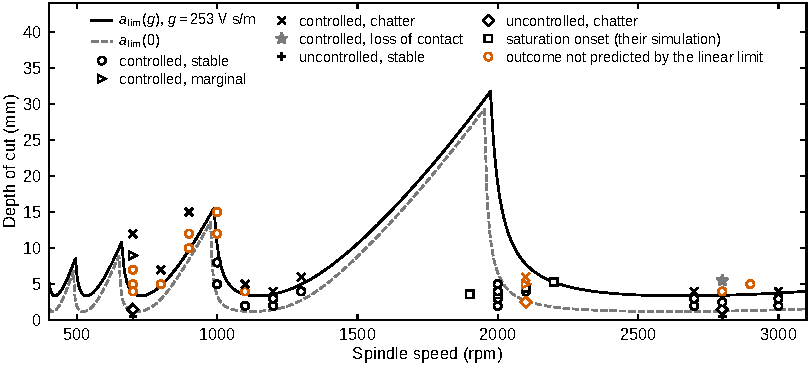
\includegraphics[width=\textwidth]{figures/fig_oz25_sld.pdf}
  \caption{The cuts of Fig.~6 of \citet{ozsoy2025frequency} (structure of Table~\ref{M-tab:case}, DVF, $g=\SI{253}{\volt\second\per\metre}$) on the linear limits of the model; orange markers: outcome not predicted by the linear limit (controlled cuts: the controlled limit; uncontrolled cuts: the uncontrolled limit); the cut with loss of contact (grey) is not classified. The squares are the onsets of saturation of the article's time-domain simulation, not tests.}
  \label{fig:oz25-sld}
\end{figure}

\subsection{Forced command, saturation and outcome of the saturation tests}\label{supp:oz25-sat}

For every test of Figs.~10 and 12 (Table~\ref{tab:oz25}), the settled forced demand $F_p=K_ag\max\lvert\dot x_p\rvert$ was computed from 40 tooth-passing harmonics of the helical force applied to the controlled receptance, which is the forced command of Section~\ref{M-sec:model-orbit} in force units ($F_p>\SI{27}{\newton}$: the forced orbit reaches the \SI{9}{\volt} clip); the alternative readings of a measured `amplitude', the amplitude of the tooth-passing harmonic and $\sqrt2$ times the RMS value, differ from $F_p$ by less than \SI{2}{\percent} median ratio. Each test was simulated with the face and the step entry, the \SI{9}{\volt} clip, the full surface memory and loss of contact, and classified by D1 over the 300 revolutions after full engagement; whether the command reached the clip at any time of the run was recorded. Between the two linear limits the critical kick was computed at the phases 0, 4, 8 and 12 of 16 with the protocol of Section~\ref{M-sec:bistab-prot}. In Table~\ref{tab:oz25}, Meas.\ is the measured amplitude of the command, or Sat where it saturated; Out.\ the measured outcome (C chatter, M marginal, otherwise stable); Pos.\ the depth relative to the limits of the model (B below $\alim(0)$, W between $\alim(0)$ and $\alim(g)$, A above $\alim(g)$); $F_p$ the predicted settled forced demand; Face and Step the simulated outcome with each entry (S settles, C chatters; $^*$: the command reaches the clip during the run); and $\Delta v^*$ the smallest critical kick over the four phases, for the tests between the limits ($\infty$: no chatter up to \SI{3}{\metre\per\second}).

\begin{table}[!htbp]
  \centering
  \caption{Saturation tests of \citet{ozsoy2025frequency} (Figs.~10 and 12) against the model (columns defined in Section~\ref{supp:oz25-sat}).}
  \label{tab:oz25}
  \scriptsize
  \setlength{\tabcolsep}{4pt}
  \renewcommand{\arraystretch}{0.84}
  \begin{tabular}{@{}rrrcrrccr@{}}
    \toprule
    $n$ & $a$ & Meas. & Out. & Pos. & $F_p$ & Face & Step & $\Delta v^*$\\
    (rpm) & (mm) & (N) & & & (N) & & & (mm/s)\\
    \midrule
1700 & 3 & 9 &  & B & 8.4 & S & S & \\
1700 & 5 & 12 &  & B & 11.4 & S & S & \\
1700 & 10 & 10 &  & B & 7.4 & S & S & \\
1700 & 15 & 5 &  & B & 7.0 & S & S & \\
1700 & 20 & 13 &  & A & 11.5 & C & C & \\
1750 & 2 & 9 &  & B & 7.4 & S & S & \\
1750 & 3 & 12 &  & B & 10.4 & S & S & \\
1750 & 5 & 14 &  & B & 14.4 & S & S & \\
1750 & 10 & 9 &  & B & 9.2 & S & S & \\
1750 & 15 & 4 &  & B & 8.8 & S & S & \\
1750 & 20 & 16 &  & A & 14.5 & C & C & \\
1800 & 0.5 & 3 &  & B & 2.5 & S & S & \\
1800 & 1.5 & 8 &  & B & 7.3 & S & S & \\
1800 & 3 & 13 &  & B & 13.6 & S & S & \\
1800 & 5 & 19 &  & B & 18.8 & S & S & \\
1800 & 10 & 15 &  & B & 12.0 & S & S & \\
1800 & 15 & 6 &  & B & 11.4 & S & S & \\
1800 & 20 & Sat &  & W & 19.0 & S & S & $\infty$\\
1800 & 22 & 19 &  & A & 14.1 & C & C & \\
1850 & 2 & 15 &  & B & 13.3 & S & S & \\
1850 & 3 & 20 &  & B & 18.8 & S & S & \\
1850 & 5 & Sat &  & B & 25.8 & S* & S & \\
1850 & 10 & Sat &  & B & 16.6 & S & S & \\
1850 & 15 & 6 &  & B & 15.8 & S & S & \\
1850 & 20 & Sat &  & B & 26.1 & S* & S & \\
1900 & 0.5 & 5 &  & B & 4.5 & S & S & \\
1900 & 1.5 & 12 &  & B & 13.2 & S & S & \\
1900 & 3 & Sat &  & B & 24.5 & S* & S & \\
1900 & 5 & Sat &  & B & 33.8 & S* & S* & \\
1900 & 10 & Sat &  & B & 21.5 & S* & S & \\
1900 & 15 & 8 &  & B & 20.6 & S* & S & \\
1900 & 20 & Sat &  & B & 34.1 & S* & S* & \\
1950 & 2 & 19 &  & B & 16.5 & S & S & \\
1950 & 3 & Sat &  & B & 23.5 & S* & S & \\
1950 & 5 & Sat &  & B & 32.7 & S* & S* & \\
1950 & 10 & Sat &  & B & 20.6 & S* & S & \\
1950 & 15 & 16 &  & W & 19.7 & S* & S* & $\infty$\\
1950 & 20 & Sat & M & W & 33.0 & S* & S* & 397\\
2000 & 2 & 14 &  & B & 12.6 & S & S & \\
2000 & 3 & 19 &  & B & 18.0 & S & S & \\
2000 & 5 & Sat &  & W & 25.0 & S* & S* & $\infty$\\
2000 & 10 & Sat & M & W & 15.7 & S & S* & 139\\
2050 & 2 & 12 &  & B & 9.7 & S & S & \\
2050 & 3 & 16 &  & B & 13.7 & S & S & \\
2050 & 5 & Sat & C & W & 18.8 & S* & S* & $\infty$\\
2050 & 10 & Sat & C & A & 12.1 & C* & C* & \\
2100 & 2 & 10 &  & B & 7.8 & S & S & \\
2100 & 3 & 13 &  & W & 10.9 & S & S & $\infty$\\
2100 & 5 & Sat & C & W & 14.8 & S & S* & $\infty$\\
2100 & 10 & Sat & C & A & 9.6 & C* & C* & \\
2150 & 2 & 7 &  & W & 6.4 & S & S & $\infty$\\
2150 & 3 & 11 &  & W & 9.0 & S & S & $\infty$\\
2150 & 5 & Sat & M & W & 12.2 & S & S & $\infty$\\
2200 & 2 & 7 &  & W & 5.5 & S & S & $\infty$\\
2200 & 3 & 18 &  & W & 7.7 & S & S & $\infty$\\
2200 & 5 & Sat & C & A & 10.3 & C & S & \\
    \bottomrule
  \end{tabular}
\end{table}
% src: verification/ozsoy2025/sim2025.py/.json (closed_form.demand_N, face/step chatter and run_clipped), compare2025.json (fig10.rows position; amplitude_h1 and amplitude_rms2 median ratios 0.888 and 0.889 against 0.903 for the peak), kicks2025.json

Of the 36 numerical values, the predicted $F_p$ is 0.90 times the measured one (median; interquartile range 0.83--1.02; correlation 0.66): 0.92 (range 0.82--1.10) at the 16 tests of up to \SI{5}{\milli\metre} at 1700--\SI{2000}{\rpm}, with absolute errors of at most \SI{2.5}{\newton}, 0.81 (range 0.43--0.92) at the 8 tests of up to \SI{5}{\milli\metre} from \SI{2050}{\rpm}, 0.80 at \SI{10}{\milli\metre}, 2.05 (range 1.23--2.64) at \SI{15}{\milli\metre} and 0.89 at 20--\SI{22}{\milli\metre}. The settled forced orbit is predicted to saturate at 4 of the 20 saturated tests (1900 and \SI{1950}{\rpm}, 5 and \SI{20}{\milli\metre}), the command reaches the clip during the simulated face entry at 12 of them and at 2 unsaturated ones (1900 and \SI{1950}{\rpm}, \SI{15}{\milli\metre}), and later in the run at 2 more saturated ones (2050 and \SI{2100}{\rpm}, \SI{10}{\milli\metre}), through simulated chatter above the controlled limit. The simulated face entry chatters exactly at the six tests above the controlled limit, of which three were measured stable; it settles at all 13 tests between the limits, of which five lost stability.
% src: verification/ozsoy2025/compare2025.json (fig10.amplitude_peak; demand_over_measured; abs_error_depth_le5_rpm_le2000_N max 2.46; saturation_settled_closed_form both 4; saturation_any_time_face_entry both 14, pred_only 2; outcome_face both 3, pred_only 3, meas_only 5)

\paragraph{Helix angle} From 1700 to \SI{1950}{\rpm} the measured command has a local minimum over the depth near \SI{15}{\milli\metre}, between the two regions of saturation, while the tooth-passing force of the \SI{45}{\degree} helix is most nearly constant at the axial pitch, $\pi D/(N_t\tan45^\circ)$, which is \SI{12.6}{\milli\metre}. Recomputed with helix angles of 36--\SI{46}{\degree}, everything else unchanged, the mean absolute logarithmic ratio of predicted to measured command at the 36 tests falls from 0.24 at \SI{45}{\degree} to 0.16 at \SI{42}{\degree} (axial pitch \SI{14.0}{\milli\metre}). This only locates the discrepancy, in the distribution of the force, or of the mode, over the depth; the model keeps the \SI{45}{\degree} of the article.
% src: verification/ozsoy2025/helix2025.py/.json (mean_abs_log 0.240 at 45, 0.159 at 42 (best), 0.164 at 43; pitch_mm 12.57 and 13.96)

\paragraph{Onset of saturation in the article's simulation} The four squares of Fig.~6, the article's time-domain onsets of saturation at 1900, 2000, 2100 and \SI{2200}{\rpm}, lie at 3.6, 3.6, 4.5 and \SI{5.3}{\milli\metre}; the forced demand of the model reaches \SI{27}{\newton} at 4.1 and \SI{5.9}{\milli\metre} at the first two speeds and not below the controlled limit at the others (\SI{13.5}{\newton} at \SI{2100}{\rpm} and \SI{4.5}{\milli\metre}; at \SI{2200}{\rpm} the square, at \SI{5.29}{\milli\metre}, lies on the model's controlled limit of \SI{5.28}{\milli\metre}). The details of that simulation are not given.
% src: verification/ozsoy2025/onset2025.py/.json (model_onset_mm 4.15, 5.90, None, None: first depth of a 0.05 mm grid with demand above 27 N; closed form 26.94 N at 4.10 mm, 27.02 N at 4.12 mm, 27.00 N at 5.85 mm; square at 2200 rpm digitised at 5.292 mm (points_fig6.json depth_measured_mm); demand_at_article_onset_N 24.8, 21.3, 13.5, 9.6; a_lim_g_mm 2200 rpm 5.280)

\section{Supplement to Section 3: authority condition}\label{supp:feas}

This section gives the settings and secondary results of Section~\ref{M-sec:feasibility}.

\subsection{Reproduction of the published condition}\label{supp:feas-pub}

The condition of Eq.~\eqref{M-eq:pub} was evaluated with the simulator of Section~\ref{app:simulator} without the clip, with single regeneration and over 50 revolutions, starting with a step entry from rest at the depth $\alim(g)$; the demand is $K_ag\max_t\lvert\dot x\rvert$ over the whole run, compared with $F_{\max}=\SI{27}{\newton}$. The gain was searched on $\mathcal G=[0,3000]$\,\si{\volt\second\per\metre} by two methods: the self-adaptive differential evolution (SADE) of \citet{qin2009sade}, with 20 individuals, at most 60 generations, a stop after 25 generations without improvement and three seeds per speed; and a deterministic reference, a scan in steps of \SI{20}{\volt\second\per\metre} refined by bisection at the edges of every feasible interval. Both evaluate the same objective, and the map takes the better result.
% src: src/objective.py (demand: K_a g max|x'|, single regeneration, N_REVS = 50), src/sade.py, src/gainmap.py (G = [0, 3000], DG = 20, reference), src/run_gain_map.py; README §2, §4.6

SADE reached the optimum at 250 of the 251 speeds. Where it and the reference differ (2280, 2300 and \SI{2310}{\rpm}), one of them missed an isolated pocket of feasible gains: the \SI{20}{\volt\second\per\metre} grid of the reference stepped over the pocket at 2300 and \SI{2310}{\rpm}, and all three seeds of SADE missed it at \SI{2280}{\rpm} (\SI{5.96}{\milli\metre} against \SI{12.03}{\milli\metre}), a property of the objective rather than a numerical error. The optimum lies in such a pocket, above an interval of rejected gains, at every speed from 2060 to \SI{2310}{\rpm} and at 670, 1010 and 1970--\SI{2000}{\rpm} (32 speeds). On the interval connected to $g=0$ the gain at 2060--\SI{2310}{\rpm} would be about 0.72 times the published one, and the depth 6.0--\SI{8.0}{\milli\metre}. Where the optimum enters or leaves a pocket the map jumps, for instance from 383 to \SI{213}{\volt\second\per\metre} between 2000 and \SI{2010}{\rpm} and from 858 to \SI{415}{\volt\second\per\metre} between 2310 and \SI{2320}{\rpm}. Over all speeds the reproduced gain ranges from \SI{71}{\volt\second\per\metre} (\SI{1950}{\rpm}) to \SI{1046}{\volt\second\per\metre}.
% src: README §5.2 (250/251; pockets; connected-interval gain 0.72 of the published); results/gainmap_main.npz (g_ref, a_ref, g_sade, a_sade, sade_runs: 2280 rpm all seeds 5.96 mm, a_ref 12.03 mm; 2300 and 2310 rpm a_ref 5.97 and 5.99 mm, SADE 11.87 and 11.80 mm; scan_g, scan_f, scan_alim, scan_fd: isolated pockets recomputed, 32 speeds; connected-interval depths recomputed with the edge bisected as in gainmap.reference: 5.96-7.96 mm, against 5.75-7.52 mm at the last feasible gain of the 20 V s/m grid; g_best 71.1-1045.7 V s/m, minimum at 1950 rpm, 383.3 -> 213.0 and 858.5 -> 414.8 V s/m)

The ratios to the published map quoted in Section~\ref{M-sec:feas-pub} use the map of Fig.~8 of \citet{ozsoy2026robust}, read from the vector graphics of that figure. The published map is straight over 500--550, 560--610 and 1410--\SI{1860}{\rpm} and is a single segment without vertices over 620--\SI{740}{\rpm}; these segments are excluded, so that the medians 0.74 and 0.88 refer to 750--1150 and 1160--\SI{1400}{\rpm}. The median ratio at 2060--\SI{2310}{\rpm} is 1.83. If the demand $g\lvert\dot x\rvert$ is read as a voltage and compared with 27, the reproduced gains become 2--3 times larger (780--\SI{1971}{\volt\second\per\metre}).
% src: verification/targets/fig8_gain_map.csv, fig8_segments.csv; README §4.4 (straight segments), §5.2, §6 (voltage reading: results/gainmap_volt.npz, g_ref 780-1971 V s/m); results/paper_vs_ours.json (p04: band medians 0.74, 0.88, 1.83, 0.97; band_note: 500-1150 is 750-1150 and 1160-1490 is 1160-1400)

With the step entry the peak demand is that of the entry transient (Section~\ref{M-sec:feas-pub}). On a grid of \SI{50}{\volt\second\per\metre} the optimum of Eq.~\eqref{M-eq:pub} at \SI{2500}{\rpm} is \SI{500}{\volt\second\per\metre} ($\alim=\SI{5.86}{\milli\metre}$) with the step entry, but \SI{2900}{\volt\second\per\metre} (\SI{38.3}{\milli\metre}) with a feed ramp of one revolution, \SI{3000}{\volt\second\per\metre} (\SI{40.0}{\milli\metre}) with a feed ramp of ten revolutions and \SI{2950}{\volt\second\per\metre} (\SI{39.2}{\milli\metre}) with a face entry.
% src: verification/paper/support_runs.json (eq2_optimum_2500rpm: step 500 V s/m, 5.86 mm; ramp1 2900, 38.29 mm; ramp10 3000, 40.03 mm; face 2950, 39.15 mm)

\subsection{The reformulated condition}\label{supp:feas-new}

By Eqs.~\eqref{M-eq:Gcl} and~\eqref{M-eq:xp}, the harmonic of $b(t)$ at $\omega=m\omega_T$ is
\begin{equation}\label{eq:supp-feas-bm}
  b_m=-g\,i\omega\,G_{\mathrm{cl}}(i\omega)\,F_m(a)=-F_m(a)\,i\omega G(i\omega)\,\frac{g}{1+gz},
\end{equation}
with $z=i\omega G_a(i\omega)G(i\omega)$. At a fixed depth, $\lvert g/(1+gz)\rvert^{-2}=(1/g+\operatorname{Re}z)^2+(\operatorname{Im}z)^2$ has the derivative $-2(1/g+\operatorname{Re}z)/g^2$ with respect to $g$, so $\lvert b_m\rvert$ in Eq.~\eqref{eq:supp-feas-bm} grows with $g$ if and only if $1+g\operatorname{Re}z>0$: at every gain for the harmonics with $\operatorname{Re}z\ge0$, and for $g<1/\lvert\operatorname{Re}z\rvert$ at the others. The steady demand $F_{\mathrm{ss}}$ of Eq.~\eqref{M-eq:feas} can therefore fall with $g$ only where this condition fails, through the phases of the harmonics, which also change with $g$ and move the peak of their sum, or through the depth range $(0,\kappa\alim(g)]$ and the 80 depths sampled evenly in it, which move with $g$. On a grid of 151 gains from 0 to \SI{3000}{\volt\second\per\metre} at all 251 speeds, $F_{\mathrm{ss}}$ increased with $g$ except for drops of at most \SI{0.22}{\newton} at 27 speeds, all at $g\ge\SI{2120}{\volt\second\per\metre}$ and at demands above \SI{140}{\newton}, far beyond $F_{\max}$, and the feasible set was one interval $[0,g_b]$ at every speed. Its upper edge was found by bisection to \SI{0.25}{\volt\second\per\metre}; SADE, applied to the same condition, improved on it by at most \SI{0.013}{\milli\metre}.
% src: Eqs. (Gcl), (xp) of the article; src/structure.py (G, Ga, Gcl), src/feasibility.py (forced_velocity, demand_envelope: N_DEPTH = 80; edge_gain: tol 0.25); verification/paper/feas_monotone.json (251 speeds x 151 gains: drops <= 0.215 N at 27 speeds, g >= 2120 V s/m, F_ss >= 144.9 N; all_one_interval true); README §8.2 (SADE better by <= 0.013 mm); results/feas_g1500.npz (a_sade - a_ref <= 0.0133 mm)

The closed form was compared with the settled demand of the simulator at the operating depth $\kappa\alim$, at the 139 speeds where that run settled. At the 129 of them whose demand is at least \SI{1}{\newton}, the simulator, with 30 axial layers, exceeds the closed form by $-0.75$ to $+\SI{8.7}{\percent}$ (median $+\SI{1.1}{\percent}$; more than \SI{3.7}{\percent} at 12 speeds), by at most \SI{0.98}{\newton} (\SI{0.33}{\volt}); at the other ten, where the helix cancels the force harmonics, the demand is below \SI{1}{\newton} and the difference at most \SI{0.06}{\newton}. At three speeds (520, 660 and \SI{1900}{\rpm}, including the two largest differences), 240 layers bring the difference within \SI{0.8}{\percent}. The difference is therefore the axial quadrature error of the simulator, whose layers are thicker than the axial wavelengths of the higher force harmonics, whereas the closed form integrates over the depth exactly.
% src: results/feas_g1500.npz (cert_stable, cert_demand_td, cert_demand_cf: 129/139 points with demand >= 1 N, -0.75 % to +8.66 %, median +1.13 %, 12 above 3.7 %, at most 0.98 N; the other 10: demand < 0.92 N, |difference| <= 0.062 N); verification/feasibility/cf_vs_td_layers.json (520, 660, 1900 rpm: +8.66, +6.97, +3.73 % with 30 layers; -0.03, -0.13, -0.79 % with 240); README §8.2

The entry check of Eq.~\eqref{M-eq:achk} simulates step entries from rest with the clipped command ($\lvert V\rvert\le\SI{9}{\volt}$) and the full surface memory, each judged over 300 revolutions by the classifier D1 (Section~\ref{app:simulator}). The depth starts at $0.225\alim=0.25\kappa\alim$ and grows by factors of 1.08 up to $\kappa\alim$; the first interval that ends in chatter is bisected to a relative \SI{0.3}{\percent}. With $\mathcal G=[0,1500]$ no shallower depth chattered where the operating depth settled, so the check binds exactly at the 112 speeds where the run at $\kappa\alim$ did not settle: at 85 speeds with $g^\star=\SI{1500}{\volt\second\per\metre}$ and at 1530--1560, 1980--2010 and 2280--\SI{2460}{\rpm}. At \SI{2500}{\rpm}, for instance, $\alim=\SI{17.24}{\milli\metre}$ and $\kappa\alim=\SI{15.51}{\milli\metre}$, but the clipped step entry chatters above \SI{13.01}{\milli\metre}. Over all speeds $\achk/\alim$ ranges from 0.74 to 0.90.
% src: src/run_feas_certify.py (a_lo = 0.25 kappa a_lim, growth 1.08, nreg = 0), src/tdboundary.py (boundary: rtol 3e-3; classify: NREV 300); results/feas_cert_g1500.npz, results/feas_g1500.npz (cert_stable = 0 at 112 speeds = 85 at g = 1500 + 27 at 1530-1560, 1980-2010, 2280-2460 rpm; no speed with cert_stable = 1 and a_cert < a_op_linear; 2500 rpm: a_lim 17.24, a_op_linear 15.51, a_td_clipped 13.01 mm; a_cert/a_lim 0.737-0.900); README §8.3

\subsection{Results by speed and sensitivity}\label{supp:feas-res}

In the range 1500--\SI{2050}{\rpm}, where the uncontrolled limit is already high and the forced resonance caps the gain, the mean $\achk$ (\SI{20.51}{\milli\metre}) is below the mean depth of Eq.~\eqref{M-eq:pub} (\SI{21.24}{\milli\metre}), although $\alim$ at the reformulated gains averages \SI{22.94}{\milli\metre} there; speed by speed, $\achk$ lies below the depth of Eq.~\eqref{M-eq:pub} at 49 of the 52 speeds from 1690 to \SI{2200}{\rpm}. Table~\ref{tab:supp-feas-table3} compares the two designs on an equal footing at the nine speeds of Table~3 of \citet{ozsoy2026robust}, with the same clipped step entry, the full surface memory and the same classifier.
% src: results/feas_cert_g1500.npz (a_cert, a_lim), results/gainmap_main.npz (a_best); README §8.4; per-speed count recomputed from these files: 49 of 52 at 1690-2200 rpm

\begin{table}[!tbp]
  \centering
  \caption{Clipped step-entry limit $a_{\mathrm{TD}}$ (\si{\milli\metre}; \SI{9}{\volt} clip, full surface memory) at the nine speeds of Table~3 of \citet{ozsoy2026robust}, with the gains $g$ (\si{\volt\second\per\metre}) of the published condition as reproduced [Eq.~\eqref{M-eq:pub}] and of the reformulated condition [Eq.~\eqref{M-eq:feas}, $\mathcal G=[0,1500]$].}
  \label{tab:supp-feas-table3}
  \begin{tabular}{@{}rrrrr@{}}
    \toprule
    & \multicolumn{2}{c}{Eq.~\eqref{M-eq:pub}} & \multicolumn{2}{c}{Eq.~\eqref{M-eq:feas}}\\
    \cmidrule(lr){2-3}\cmidrule(l){4-5}
    Speed (rpm) & $g$ & $a_{\mathrm{TD}}$ & $g$ & $a_{\mathrm{TD}}$\\
    \midrule
    500  & 829  & 12.1 & 1500 & 17.0\\
    560  & 1043 & 10.9 & 1500 & 16.2\\
    600  & 990  & 11.1 & 1500 & 15.7\\
    800  & 1026 & 10.9 & 1500 & 15.5\\
    1300 & 992  & 11.1 & 1500 & 14.3\\
    2300 & 849  & 12.1 & 1085 & 13.5\\
    2500 & 536  & 6.37 & 1500 & 13.0\\
    2800 & 668  & 7.33 & 1500 & 12.6\\
    3000 & 712  & 8.12 & 1500 & 12.8\\
    \bottomrule
  \end{tabular}
\end{table}
% src: results/table3_main.csv (g_prop, a_prop_td), results/feas_compare_g1500.json (table3: g_new, a_new_td); both with the 9 V clip and the full surface memory (feasibility.NREG = 0)

The margin $\kappa$ hardly matters: with $\kappa=0.95$ the gains change by at most \SI{0.53}{\volt\second\per\metre}, and the same 157 speeds sit at the bound. A guard of $0.85F_{\max}$ (\SI{23}{\newton}) lowers the gain at 116 speeds, 22 of which sat at the bound with a demand of 23.1--\SI{26.8}{\newton}; the gain then ranges from 101 to \SI{1500}{\volt\second\per\metre}, with 135 speeds at the bound. The cap of $\mathcal G$ matters more: with $g_{\max}=\SI{3000}{\volt\second\per\metre}$ the steady demand binds at 195 speeds and the gain reaches the bound at 56; the mean checked depth rises to \SI{17.1}{\milli\metre}, and the entry check binds at 184 speeds. At seven of these (570--\SI{990}{\rpm}) a shallower depth, 0.55--0.69 of the operating depth, chatters while the operating depth settles, which is why a ladder of depths is simulated.
% src: results/feas_k095.npz (at_bound 157, the same speeds as feas_g1500.npz; gains within 0.53 V s/m), results/feas_guard085.npz (116 speeds lowered, 22 of them at the bound in feas_g1500.npz with demand_ref 23.1-26.8 N; g_best 100.7-1500 V s/m; at_bound 135), results/feas_g3000.npz (at_bound 56; demand binds at 195), results/feas_cert_g3000.npz (mean a_cert 17.13 mm; a_cert < a_op_linear at 184 speeds; at 570, 580, 590, 630, 770, 780 and 990 rpm the run at a_op_linear settled, cert_stable = 1, while a_td_clipped/a_op_linear = 0.55-0.69); README §8.5, §8.6

% Moved from Section 3 of the long version (sections/s3_feasibility.tex) to keep the article at standard length.
% Text copied verbatim; only references are adapted (M- = main article; no prefix = Supplementary Material).
% The displayed equations eq:pub, eq:feas and eq:achk stay in the article; here they are cited with the prefix M-.

\subsection{The published condition: full text}\label{supp:std-feas-pub}

\citet{ozsoy2026robust} schedule $g$ over the spindle speed by maximising $\alim(\Omega,g)$ subject to an authority condition. Section~\ref{M-sec:feasibility} shows that the published form of that condition, as reproduced here, measures the entry transient, and replaces it by a condition on the steady forced command, which is the part of the authority that the forced orbit takes; the rest, $\Vmax-\bmax$, is what Sections~\ref{M-sec:bistability}--\ref{M-sec:basin-aware} are about.

The published condition, Eq.~(2) of \citet{ozsoy2026robust}, simulates the cut at $a=\alim(\Omega,g)$ and accepts $g$ if the peak demand stays within the actuator rating [Eq.~\eqref{M-eq:pub}], with $g^\star(\Omega)=\arg\max_{g\in\mathcal G}J(g)$. The demand, written there as $g\lvert\dot x\rvert$ and compared with \SI{27}{\newton}, is read here as the force of Eq.~\eqref{M-eq:pub}; read as a voltage, it would make the gains 2--3 times larger. Neither the start of the simulation nor the search interval is stated. A step entry from rest (full engagement at $t=0$, zero history) reproduces the published gains at \SIrange{2320}{3000}{\rpm} (median ratio 0.97) and was used; elsewhere the reproduced gains are 0.27--1.9 times the published ones (Fig.~\ref{fig:feas}a; Section~\ref{supp:feas-pub}). With this start the peak demand is that of the entry transient: at \SI{2500}{\rpm} and $g=536$ the peak per revolution falls from \SI{27}{\newton} in the first revolution to \SI{16}{\newton} in the fiftieth, and with a feed ramp or a face entry (Section~\ref{M-sec:bistab-prot}) the optimum becomes 2900--\SI{3000}{\volt\second\per\metre} ($\alim=38$--\SI{40}{\milli\metre}) instead of 536. As the depth moves with $g$ and the forced response oscillates in the depth [Eq.~\eqref{M-eq:Fm}], the demand is not monotone in $g$, and the feasible set of the reproduced condition fragments into pockets, which hold the optimum throughout 2060--\SI{2310}{\rpm}.
% src: src/objective.py (demand K_a g max|x'|), src/gainmap.py, src/run_gain_map.py; README §2, §4.6 (start not stated; demand read as a force), §5.2 (gain ratio 0.97 at 2320-3000 rpm); results/paper_vs_ours.json (p04: band medians 0.74, 0.88, 1.83, 0.97; band_1870_2050_range 0.27-1.3); recomputed from gainmap_main.npz g_best and fig8_gain_map.csv: range 1.19-1.91 at 2060-2310 rpm; verification/claim_audit/claim_audit.json (27.0 N in rev 0 -> 16.0 N in rev 49 at 2500 rpm, g = 536); verification/paper/support_runs.json (Eq. 2 optimum at 2500 rpm: feed ramp 1 rev 2900 V s/m, 38.29 mm; 10 rev 3000, 40.03 mm; face entry 2950, 39.15 mm); README §5.2 (pockets at all of 2060-2310 rpm), §8.1

\subsection{A steady-state authority condition: full text}\label{supp:std-feas-new}

The reformulated condition requires that, once the cut has settled, the command stays inside the clip at every depth the gain admits, up to a margin $\kappa<1$ below the stability limit. Below $\alim$ the settled motion is the forced orbit of Eq.~\eqref{M-eq:xp}, so the condition has a closed form [Eq.~\eqref{M-eq:feas}], with $\kappa=0.9$ and $\mathcal G=[0,g_{\max}]$, $g_{\max}=1500$ or \SI{3000}{\volt\second\per\metre}. On a grid of gains the feasible set was one interval $[0,g_b]$ at every speed, and $g^\star=g_b$ was found by bisection. The maximum over the depth was taken over 80 evenly spaced depths; a search over 2000 depths finds it larger by at most \SI{0.12}{\percent} (\SI{14}{\milli\newton}), which would lower the gain by at most \SI{0.44}{\volt\second\per\metre} and the linear limit by at most \SI{0.015}{\milli\metre} at the 94 speeds where the authority binds. The closed form matches the simulator's settled demand to within the latter's axial quadrature error (Section~\ref{supp:feas-new}).
% src: src/feasibility.py (KAPPA = 0.9, N_DEPTH = 80, demand_envelope, edge_gain); README §8.2; verification/paper/feas_monotone.json (251 speeds x 151 gains: all_one_interval true); results/feas_g1500.npz (cert_demand_td vs cert_demand_cf), verification/feasibility/cf_vs_td_layers.json; dense check: verification/paper/protocol_eq14_sampling.json (underestimate.total_rel_max 1.16e-3 at 660 rpm, total_abs_max_N 0.0139 at 1850 rpm; gains.linearised_drop_max_Vspm 0.437, linearised_alim_drop_max_mm 0.0149; n_binding 94; top-speed bisection changes <= 0.37 V s/m)

The steady condition cannot see the entry. Each scheduled gain was therefore checked by step entries from rest with the clipped command and the full surface memory (Section~\ref{M-sec:bistab-prot}), on a ladder of depths from $0.225\alim$ in steps of \SI{8}{\percent} up to $\kappa\alim$. The clipped limit $a_{\mathrm{TD}}(g^\star)$ found in this way defines the checked depth $\achk$ of Eq.~\eqref{M-eq:achk}, which rests on the simulation of one entry and is not a certificate.
% src: src/run_feas_certify.py (a_lo = 0.25 kappa a_lim, growth 1.08, nreg = 0); src/tdboundary.py (boundary); README §8.3

\subsection{Results: full text}\label{supp:std-feas-res}

The reformulated map, with $\mathcal G=[0,1500]$, has no jumps (Fig.~\ref{fig:feas}a). Its gain sits at this chosen bound at 157 of the 251 speeds; elsewhere (1530--\SI{2460}{\rpm}) the steady demand binds, and the gain dips to \SI{135}{\volt\second\per\metre} at \SI{1940}{\rpm}, where the tooth-passing frequency matches the natural frequency. The entry check binds at 112 speeds. Averaged over all speeds (Table~\ref{tab:feas}, Fig.~\ref{fig:feas}b), $\achk=\SI{15.87}{\milli\metre}$, against \SI{12.75}{\milli\metre} for $\alim$ at the gains of Eq.~\eqref{M-eq:pub}, which carries no margin, and \SI{5.85}{\milli\metre} without control; only at 1500--\SI{2050}{\rpm}, near the forced resonance, is the mean $\achk$ below the depth of Eq.~\eqref{M-eq:pub}.
% src: results/feas_g1500.npz (at_bound: 157; g_best < 1500 over 1530-2460 rpm, minimum 134.9 V s/m at 1940 rpm); results/feas_cert_g1500.npz (a_cert < a_op_linear at 112 speeds; mean 15.87 mm), results/feas_g1500.npz (a_unc: mean 5.85 mm), results/gainmap_main.npz (a_best: mean 12.75 mm); README §8.3, §8.4

\begin{table}[!tbp]
  \centering
  \caption{Mean depths (\si{\milli\metre}) by speed range: checked depth $a_{\mathrm{chk}}$ of the reformulated condition [Eqs.~\eqref{M-eq:feas}--\eqref{M-eq:achk}, $\mathcal G=[0,1500]$, $\kappa=0.9$], $a_{\lim}$ at the gains of Eq.~\eqref{M-eq:pub} (no margin), and the uncontrolled limit $a_{\lim}(0)$.}
  \label{tab:feas}
  \begin{tabular}{@{}lrrrr@{}}
    \toprule
    Speeds (rpm) & Number & $a_{\mathrm{chk}}$ & $a_{\lim}$, Eq.~\eqref{M-eq:pub} & $a_{\lim}(0)$\\
    \midrule
    500--1150  & 66  & 16.75 & 12.36 & 4.02\\
    1160--1490 & 34  & 14.89 & 11.49 & 3.87\\
    1500--2050 & 56  & 20.51 & 21.24 & 16.58\\
    2060--3000 & 95  & 12.87 & 8.47  & 1.51\\
    All        & 251 & 15.87 & 12.75 & 5.85\\
    \bottomrule
  \end{tabular}
  \par\smallskip
  \parbox{0.9\linewidth}{\footnotesize Sensitivity (Section~\ref{supp:feas-res}): with $\kappa=0.95$ the gains change by at most \SI{0.53}{\volt\second\per\metre}; a guard of $0.85F_{\max}$ lowers the gain at 116 speeds; with $g_{\max}=3000$ the mean $\achk$ is \SI{17.1}{\milli\metre} and the entry check binds at 184 speeds.}
\end{table}
% src: results/feas_cert_g1500.npz (a_cert), results/gainmap_main.npz (a_best), results/feas_g1500.npz (a_unc); README §8.4; note: results/feas_k095.npz (gains within 0.53 V s/m), results/feas_guard085.npz (116 speeds lowered), results/feas_cert_g3000.npz (mean a_cert 17.13 mm; a_cert < a_op_linear at 184 speeds); README §8.5

The reformulated condition does not depend on the entry, but it gives up what the published one provides for a specified entry: keeping that entry inside the linear range at $a=\alim$. Nor does it say how large a disturbance the settled cut tolerates: $\achk$ lies inside the band of depths at which a kick can tip the settled cut into chatter at 104 of the 109 speeds where that band was found (Section~\ref{M-sec:bistab-map}), so a checked depth is not a safe depth. Sections~\ref{M-sec:bistability} and~\ref{M-sec:certificates} measure and bound the tolerated disturbance, and Section~\ref{M-sec:basin-aware} puts it into the schedule.
% src: results/c1_band.npz vs results/feas_cert_g1500.npz (104/109)

\begin{figure}[!tbp]
  \centering
  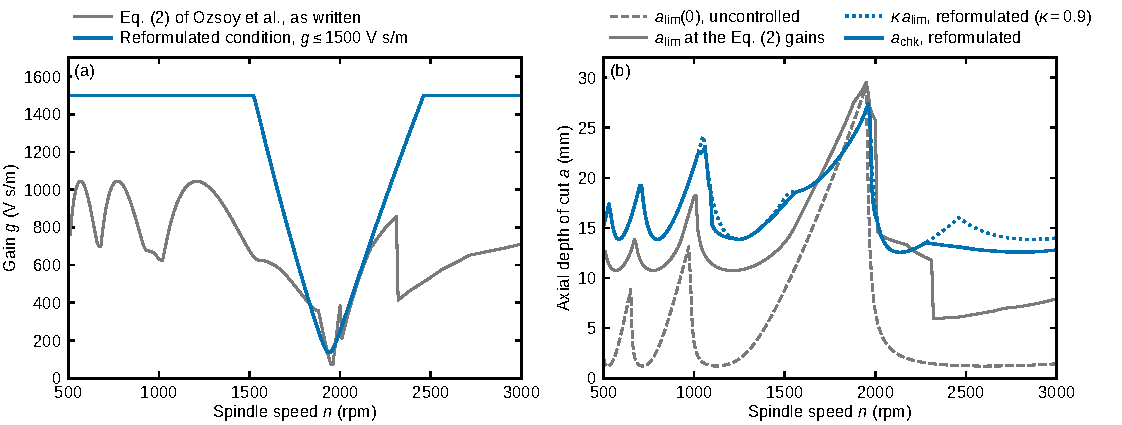
\includegraphics[width=0.86\textwidth]{figures/fig02_feasibility.pdf}
  \caption{Gain scheduling under the two authority conditions over \SIrange{500}{3000}{\rpm}. (a)~Gain maps: the published condition, Eq.~\eqref{M-eq:pub}, reproduced with a step entry, the reformulated condition, Eq.~\eqref{M-eq:feas} with $\mathcal G=[0,1500]$, and the published map of \citet{ozsoy2026robust} (dotted where it is a straight line between optimised speeds: 500--550, 560--740 and 1410--\SI{1860}{\rpm}). (b)~Depths: uncontrolled limit $a_{\lim}(0)$, $a_{\lim}$ at the gains of Eq.~\eqref{M-eq:pub}, $\kappa a_{\lim}$ and the checked depth $a_{\mathrm{chk}}$ of Eq.~\eqref{M-eq:achk} at the reformulated gains.}
  \label{fig:feas}
\end{figure}

\section{Supplement to Section 4: finite-amplitude instability}\label{supp:bistab}

This section gives the protocol details and secondary results of Section~\ref{M-sec:bistability}.

\subsection{Entries, kicks and surface memory}\label{supp:bistab-prot}

In the face entry a point of the cutting edge at angle $\phi$ is in the material once the tool centre has advanced by $R(1-\sin\phi)$, so that full engagement is reached after $R/f_z=160$ teeth (40 revolutions). A depth ramp was not used, because a real axial ramp-in shifts the regeneration delay through the helix. The depth ladder of Section~\ref{supp:std-bistab-prot} starts at $0.25\alim$ and rises in steps of \SI{8}{\percent} up to $1.05\alim$; the first interval that ends in chatter is bisected to a relative \SI{0.3}{\percent}.
% src: src/tdsim.c (opt[1]-opt[3]: ramp_f, f0, edge), src/tdsim.py (entry_revs), src/c1_unsafe_zone.py (ENTRIES, LADDER: growth 1.08, lo 0.25, hi 1.05), src/tdboundary.py (boundary: rtol 3e-3); README §11.2

The critical kick was searched upwards on a grid of 16 kicks, $\SI{0.1}{\milli\metre\per\second}\times2^k$ ($k=0,\dots,14$) and \SI{3}{\metre\per\second} (a swing of about \SI{3.7}{\milli\metre}), and only the first interval that ended in chatter was bisected, six times in $\log\Delta v$ (resolution \SI{1.1}{\percent}). The lower edge of the unsafe band was located by six bisection steps on $[0.05,0.98]\,\alim$; at each step seven kicks, spaced geometrically from \SI{3}{\milli\metre\per\second} to \SI{3}{\metre\per\second}, were applied at two phases half a tooth period apart. The bisection assumes that the band has no holes in depth. At $0.98\alim$ the slowest mode decays by only 0.985--0.994 per tooth period, so a residual of the face entry at full engagement (revolution 40) decays to 3--\SI{22}{\percent} of its value by the kick at revolution 100. Measured on the unkicked run, the deviation from the forced orbit is at most \SI{5.2}{\nano\metre} at revolution 40, \SI{0.85}{\nano\metre} at revolution 100 and \SI{0.01}{\nano\metre} at revolution 300 (Section~\ref{supp:bistab-checks}).
% src: src/c1_unsafe_zone.py (DV_GRID = 1e-4 x 2^k, k = 0..14, and 3 m/s; N_BISECT = 6; BAND_DV = geomspace(3e-3, 3, 7); BAND_PHASES = 2 at offsets 0 and ND/2; BAND_BISECT = 6 on [0.05, 0.98]; KICK_REV = 100); 3 m/s / omega_n = 3.69 mm; 2^(1/64) = 1.011; results/c1_basin.npz (decay at 0.98 a_lim: 0.9937, 0.9854, 0.9933, 0.9925 at 1090, 1420, 2500, 2870 rpm; decay^240 = 0.22, 0.029, 0.20, 0.16 over the 60 revolutions = 240 tooth periods between revolutions 40 and 100)

A kick displaces the workpiece by about $\Delta v/\omega_n$, \SI{37}{\micro\metre} for \SI{30}{\milli\metre\per\second}, less than one feed, but the clipped chatter that it releases reaches 0.08--\SI{2.0}{\milli\metre} peak to peak (Section~\ref{M-sec:bistab-attr}), up to some forty feeds, and a kick of \SI{3}{\metre\per\second} alone swings the workpiece by about 74 feeds, so the tool leaves the cut for many passes. Four remembered passes cover only \SI{0.2}{\milli\metre} of feed; with them, two of the four clipped-chatter cases of Section~\ref{app:simulator} exceed the \SI{1}{\centi\metre} at which the simulator stops where the full memory stays bounded, and a third is \SI{27}{\percent} too large. Even with the full memory a run can exceed \SI{1}{\centi\metre}, because the chip is not limited when the tool plunges into the material, for instance the step entry at \SI{1050}{\rpm} and $0.9\alim$, where the brute-force reference does so as well; with the stop raised to \SI{10}{\centi\metre}, that run returns to the forced orbit after an excursion of \SI{15}{\milli\metre} (Section~\ref{supp:bistab-attr}).
% src: verification/tdsim/check9_full_memory.json (bounded chatter 0.4345 and 0.5896 mm; nreg 4: 2350 rpm and 1090 rpm diverge where full memory is bounded, 2500 rpm 0.554 vs 0.435 mm; 1050 rpm, a = 24.18 mm = 0.9 a_lim, diverges with full memory and with the 600-pass brute force); 30 mm/s / omega_n = 36.9 um, 3 m/s / omega_n = 3.69 mm = 74 f_z; 4 f_z = 0.2 mm; README §11.2

\subsection{Two outcomes and entry limits}\label{supp:bistab-map}

In Fig.~\ref{M-fig:two} the command of the forced orbit lies between $-6.24$ and \SI{5.49}{\volt}; after the kick of \SI{7.6}{\milli\metre\per\second} the displacement settles between $-393$ and \SI{356}{\micro\metre}, with the command switching between $\pm\Vmax$. Over the 16 phases the critical kick at this depth is \SIrange{7.2}{8.8}{\milli\metre\per\second}. After the kick of \SI{7.0}{\milli\metre\per\second} the command still reaches the clip repeatedly while the deviation decays. A kick of \SI{30}{\milli\metre\per\second} on the settled cut at \SI{15}{\milli\metre} ends in chatter with the clip but decays without it.
% src: paper/figures/figure_numbers.json (fig03: orbit_V -6.24..5.49 V, chatter_x_um -393..356, chatter_V -9..9 V); results/c1_basin.npz (2500 rpm, 0.9 a_lim, clipped: range 7.21-8.76 mm/s); README §11.3

Where the step entry binds, the better of the face entry and the feed ramp gains \SI{2.51}{\milli\metre} on average; the largest gain, \SI{4.74}{\milli\metre}, is at \SI{1980}{\rpm} (\SI{19.0}{\milli\metre} for the step entry against \SI{23.8}{\milli\metre}), and at \SI{2500}{\rpm} the limits are 13.0 and \SI{17.25}{\milli\metre}. At 500, 540, 670, 720, 1000 and \SI{1080}{\rpm} the face entry and the feed ramp, and at 500, 550, 670 and \SI{1000}{\rpm} the clipped step entry, reached the top of the depth ladder, $1.05\alim$; at the other 245 speeds the mean face-entry limit is \SI{18.20}{\milli\metre} against a mean $\alim$ of \SI{18.21}{\milli\metre}. Without the clip the step-entry limit exceeds $\alim$ by more than \SI{1.5}{\percent} at 75 speeds, among them every speed from 1990 to \SI{2480}{\rpm}, and by at least \SI{5}{\percent}, the top of the depth ladder, at \SI{2000}{\rpm}. Near the forced resonance (\SIrange{1970}{2030}{\rpm}) runs of 2000 revolutions place the onset at 1.004--$1.012\alim$, so the excess there is the bias of the classifier; at the other speeds it was not checked with long runs. No unsafe band was found at 17 speeds: 500, 540 and \SI{720}{\rpm} ($g=\SI{1500}{\volt\second\per\metre}$) and 1660--1800 and \SIrange{1840}{1940}{\rpm}, where the gain is \SIrange{135}{979}{\volt\second\per\metre}.
% src: results/c1_summary.json (map: soft_minus_step_mean_mm 2.51, at_2500: step_clip 13.0, edge_clip 17.25); results/c1_map.npz recomputed: largest gain 4.741 mm at 1980 rpm (a_step_clip 19.02 mm, max(a_edge_clip, a_feed_clip) 23.76 mm); a_edge_clip and a_feed_clip = 1.05 a_lim at 500, 540, 670, 720, 1000, 1080 rpm, a_step_clip at 500, 550, 670, 1000 rpm; a_step_free/a_lim > 1.015 at 75 speeds (1.0165-1.050, all of 1990-2480 rpm, 1.050 at 2000 rpm); verification/tdsim/check10_forced_resonance_long_runs.json (onset 1.0039-1.0121 at 1970-2030 rpm); results/c1_summary.json (band: none_at_rpm, g_where_none 135-979 V s/m)

\subsection{Basin without the clip and near the limit}\label{supp:bistab-basin}

Worst-phase kicks of at most \SI{10}{\milli\metre\per\second} end in chatter from 0.95, 0.90 and $0.95\alim$ upwards at 1420, 2500 and \SI{2870}{\rpm} and at none of the 12 depths at \SI{1090}{\rpm}; kicks of at most \SI{30}{\milli\metre\per\second} from 0.40, 0.80, 0.40 and $0.50\alim$ upwards at 1090, 1420, 2500 and \SI{2870}{\rpm}. Over the 16 phases the critical kick varies by at most \SI{15}{\percent} at $0.98\alim$ and \SI{24}{\percent} at any depth.
% src: results/c1_basin.npz recomputed: smallest depth with worst-phase dv <= 10 mm/s: 0.95, 0.90, 0.95 a_lim at 1420, 2500, 2870 rpm, none at 1090; <= 30 mm/s: 0.40, 0.80, 0.40, 0.50 a_lim at 1090, 1420, 2500, 2870 rpm; results/c1_summary.json (basin: phase_spread_098, phase_spread_max)

Without the clip, kicks of 0.78, 3 and \SI{1.64}{\metre\per\second}, each in one phase of 16, ended in chatter at \SI{1090}{\rpm} and 0.9 and $0.98\alim$ and at \SI{2500}{\rpm} and $0.98\alim$; there the clip shrinks the basin by factors of 52, 276 and 701. At nine further points the clipped cut chatters but the unclipped cut did not for any kick up to \SI{3}{\metre\per\second}, so the factor is at least 70--595 (Fig.~\ref{M-fig:basin}). At the four remaining, shallow points (\SI{1420}{\rpm} at 0.3 and $0.6\alim$; 2500 and \SI{2870}{\rpm} at $0.3\alim$) no kick up to \SI{3}{\metre\per\second} ends in chatter, with or without the clip.
% src: results/c1_basin.npz (vmax = 0 rows: finite minima 0.784, 3.000, 1.638 m/s, one phase each; ratios of the smallest unclipped to the smallest clipped kick 52.1, 275.7, 700.9; lower bounds 3 m/s / clipped minimum 69.7-594.9 at the nine points listed); README §11.5

At $0.999\alim$, with the same protocol at four phases a quarter of a tooth period apart, the critical kick is \SIrange{1.41}{1.47}{\milli\metre\per\second} at \SI{2500}{\rpm}, \SIrange{7.1}{7.6}{\milli\metre\per\second} at \SI{2870}{\rpm} and \SIrange{9.1}{10.5}{\milli\metre\per\second} at \SI{1090}{\rpm}; \SI{1420}{\rpm} was not simulated at this depth.
% src: verification/tdsim/check11_kick_near_limit.json (phases 0, 4, 8, 12 of 16; 1.405-1.467, 7.055-7.611, 9.150-10.533 mm/s)

\subsection{Attractors beyond the basin}\label{supp:bistab-attr}

\paragraph{Long runs after a kick} At the 29 clipped points of Fig.~\ref{M-fig:basin} with a finite critical kick, the settled cut was kicked at revolution 100 of a face entry, at the phase with the smallest stored critical kick $\Delta v^*$, with 2, 2.5 and 3 times $\Delta v^*$ (at most \SI{3}{\metre\per\second}), and run for 2000 revolutions after the kick with the full surface memory. A run returned to the forced orbit if $\max\lvert x(t)-x(t-T)\rvert<0.01f_z$ over its last quarter; it ended in bounded, stationary chatter if, between revolutions 500--1000 and 1500--2000, the root mean square of $x$ and of $V$ differed by less than \SI{10}{\percent}, the fraction of clipped time by less than 0.05 and the dominant non-synchronous frequency by less than \SI{1}{\hertz}; it was stopped if $\lvert x\rvert$ exceeded \SI{1}{\centi\metre}. All 87 runs ended in bounded, stationary chatter, which the 300-revolution classifier had also called chatter. The four points at $0.9\alim$ were continued to 4000 revolutions.

\paragraph{Bifurcation-type diagrams} At 1090, 1420, 2500 and \SI{2870}{\rpm}, with the gain $g=\SI{1500}{\volt\second\per\metre}$, 28 depths evenly spaced from $\alim(0)$ to $1.05\alim$ were started by a face entry, by the face entry with a kick of 0.03 or \SI{0.3}{\metre\per\second} at revolution 100 (start of a tooth period), and by a step entry, and run for 1600 revolutions. The final state over the last 300 revolutions was the forced orbit, bounded chatter (stationary to \SI{10}{\percent}), a transient or an excursion beyond \SI{1}{\centi\metre}; only the first two occurred. The lowest grid depth reached by chatter was refined by five bisection steps against the depth below it, at each step with the seven kicks of the band study; as reaching the chatter branch from one of these starts is sufficient but not necessary, the refined end is an upper bound of the end of the branch.

\paragraph{Regularity} Twin runs whose kicks (four points at $0.9\alim$, 2000 revolutions) or depths (step entries at $1.05\alim$ at the four speeds and at two further cases, 1600 revolutions) differ by a relative $10^{-9}$ stay within $5\times10^{-7}$ of the peak-to-peak displacement of the chatter at the end, and their separation does not grow exponentially at any point: the chatter is regular, quasi-periodic where its Poincar\'e section is a closed curve.

\paragraph{Spot check} At the speeds of the band map with a band edge and $\alim\ge\SI{21}{\milli\metre}$, and at \SI{1050}{\rpm}, where the check of the surface memory had exceeded \SI{1}{\centi\metre} (700, 960, 980, 1000, 1020, 1040, 1050, 1060, 1080, 1620, 1640, 1820, 1960 and \SI{1980}{\rpm}, with the gains of Section~\ref{M-sec:feasibility}), the step entry and kicks of 0.03 and \SI{0.3}{\metre\per\second} at the start of revolution 100 of a face entry were run for 1600 revolutions at 0.9 and $0.98\alim$, and at $0.99\alim$ where the band edge lies above $0.9\alim$, at depths above the band edge only. Of 78 runs, 34 ended on the forced orbit, 23 in bounded chatter of 0.04--\SI{2.9}{\milli\metre} peak to peak, and 21 diverged, all of the latter at 700 and 1020--\SI{1060}{\rpm}.
% src: verification/paper/attractors_kick.py/.json (protocol, summary), attractors_bifurcation.py/.json/.npz (protocol, refine_lo/hi), attractors_chaos.py/.json (10 cases regular; sep_final_over_pp <= 4.9e-7), attractors_band_spot.py/.json (14 speeds, 78 runs: forced 34, chatter 23, diverged 21; bounded_pp_x_mm 0.044-2.94; speeds_with_divergence 700, 1020-1060)

\subsection{Checks of the protocols}\label{supp:bistab-checks}

\paragraph{Kick timing} At $0.98\,\alim$, where the chatter mode decays slowest, the face entry leaves at revolution 100 a deviation from the forced orbit of at most \SI{0.85}{\nano\metre} and \SI{0.73}{\micro\metre\per\second}, three orders of magnitude below the smallest critical kick. Kicking at revolution 300 instead of 100, at four phases a quarter of a tooth period apart at each of the four speeds, changes the critical kick at one of the 16 speed--phase pairs, by \SI{1.1}{\percent} (one bisection step), and its minimum over the phases at none.

\paragraph{Window} Judged over 900 instead of 300 revolutions after the kick, the 53 runs of the worst-phase searches at $0.98\,\alim$ get the same verdicts, and the critical kick is unchanged at the four speeds. The bias of the 300-revolution window found for step-entry limits near the forced resonance (Section~\ref{M-sec:bistab-prot}) does not reach the kick-based results, because after a kick the chatter grows or decays within some tens of revolutions (Fig.~\ref{fig:attr}g).

\paragraph{Phases} The critical kick at $0.98\,\alim$ was searched at the 48 phases between those of the stored campaign, i.e.\ at 64 phases per tooth period. The minimum over the phases falls by \SI{1.1}{\percent} at \SI{1090}{\rpm} (from 10.88 to \SI{10.76}{\milli\metre\per\second}, a value already reached with 32 phases) and is unchanged at the other three speeds; the spread over the phases grows from 13.9 to \SI{15.1}{\percent} at \SI{1090}{\rpm} and is unchanged elsewhere.

\paragraph{Holes in the band} At nine speeds spread over the range of the band (640, 960, 1640, 1820, 1000, 2140, 2800, 1300 and \SI{520}{\rpm}; first those where the stored edge jumps between neighbouring speeds or lies at the top of the bisection interval, then evenly spread ones), with the gains of the band map, each depth $0.05,0.10,\dots,0.95$ and $0.98\,\alim$ was tested exactly as one bisection step of the band protocol: the seven kicks from \SI{3}{\milli\metre\per\second} to \SI{3}{\metre\per\second} at two phases half a tooth period apart, stopping at the first chatter; 2028 runs in all. At every speed the lowest chattering grid depth lies directly above the bisection bracket of the stored edge, or inside it at 1000, 1640 and \SI{1820}{\rpm}, and no grid depth below the edge chatters. At eight speeds the chattering depths form one interval up to $0.98\,\alim$. At \SI{520}{\rpm} ($g=1500$, $\alim=\SI{18.4}{\milli\metre}$, edge $0.30\,\alim$) they do not: kicks end in chatter at 0.30--$0.55\,\alim$ and at 0.95 and $0.98\,\alim$, but at none of the seven grid depths from 0.60 to $0.90\,\alim$. The bisection of the band map assumes one interval; where this fails, the mapped edge is still the lowest depth at which a kick of the protocol ends in chatter, but the band above it is not unsafe throughout. Whether other kicks or phases would end in chatter inside the hole was not examined.
% src: verification/paper/protocol_band_holes.py/.json (protocol: SPEEDS order, FRACS 0.05:0.05:0.95 and 0.98, BAND_DV and BAND_PHASES of src/c1_unsafe_zone.py, face entry, kick at revolution 100, 300-revolution window, full memory; summary.*: grid_edge_frac 0.80/0.90/0.98/0.98/0.35/0.45/0.45/0.60/0.30 against stored_edge_frac 0.791/0.893/0.980/0.980/0.355/0.442/0.428/0.588/0.297; ambiguous_in_bracket at 1640, 1820, 1000 rpm; chatter_below_edge [] at all; chatter_set_is_interval_on_grid false only at 520 rpm: chatter_fracs 0.30-0.55, 0.95, 0.98, holes_above_edge 0.60-0.90; a_lim 18.45 mm; total_runs 2028)
% src: verification/paper/protocol_kick_timing.py/.json (units.residual_*: dev_x_from_orbit_um at rev100 <= 0.00085, dev_v_from_orbit_mmps <= 0.00073; summary.all: 16 points, ratio 0.989-1, max_abs_rel_change 0.0108; per speed ratio_of_minima 1.0); verification/paper/protocol_window.py/.json (summary: 4 points, 53 runs, n_disagreeing_runs 0, ratio 1.0); verification/paper/protocol_phases.py/.json (summary: n_phases_available 64; 1090 rpm min_16 10.881, min_32 10.763, min_64 10.763 mm/s, rel_change_of_min -0.0108, spread_16 0.139, spread_available 0.151; 1420, 2500, 2870 rpm rel_change 0, spread unchanged)

\subsection{Describing function and gain plane}\label{supp:bistab-df}

Equation~\eqref{M-eq:df} was evaluated as the average over one tooth period and over the phase of the chatter component, on $128\times128$ samples. The factor $p$ was fitted on the unclipped cut kicked by \SI{1}{\milli\metre\per\second} at the start of a tooth period: the velocity deviation from the unkicked run was high-passed at \SI{40}{\hertz}, which removes the actuator mode, and the per-tooth peak of the deviation, once the faster modes had died out, was fitted by the slowest mode and extrapolated back to the kick; fits with $r^2<0.98$ were discarded, which left $p$ from $0.7\alim$ upwards ($0.8\alim$ at \SI{1420}{\rpm}). On a machine, $p$ could be estimated from a measured frequency response as the residue of the critical root of Eq.~\eqref{M-eq:char}; this was not attempted.
% src: src/c1_unsafe_zone.py (df_gain: _TH 128 phases, b on ND = 128 samples per tooth period; _mode_factor: dv0 = 1e-3 m/s at the start of revolution 100, F_HP = 40 Hz, k0 = 6, r2 >= 0.98); results/c1_basin.npz (p_mode finite from 0.7 a_lim, 0.8 a_lim at 1420 rpm)

At \SI{1090}{\rpm} the clipped step-entry limit stays at \SIrange{19.3}{19.9}{\milli\metre} for $g\ge\SI{1650}{\volt\second\per\metre}$ (\SI{18.8}{\milli\metre} at $g=1500$), and at \SI{2500}{\rpm} at \SIrange{13.0}{13.2}{\milli\metre} for $g\ge1500$. The face entry follows $\alim$ until the forced command itself exceeds the clip at some depth below $\alim$: from $g=1650$ at \SI{2500}{\rpm}, after which its limit stays at \SIrange{16.7}{17.9}{\milli\metre}, and only at $g=3000$ at \SI{1090}{\rpm} (\SI{40.4}{\milli\metre} against $\alim=\SI{41.8}{\milli\metre}$). Below the plateau the clipped step-entry limit rises monotonically with the gain at both speeds; at \SI{2500}{\rpm} it is 6.4, 8.8 and \SI{13.0}{\milli\metre} at $g=536$, 800 and \SI{1500}{\volt\second\per\metre}.
% src: results/c1_gainplane.npz (gains 0-3000 in steps of 150; a_step_clip monotone in g at both speeds; a_edge_clip, a_lim, orbit_peak_V: 9.21 V at g = 1650, 2500 rpm; 9.16 V at g = 3000, 1090 rpm), results/c1_summary.json (gainplane); results/table3_main.csv (2500 rpm: a_prop_td 6.373 mm at g = 535.6, a_clip1500_td 13.010 mm), results/table3_clip_gain_sweep.csv (8.771 mm at g = 800); README §5.5, §11.6

% Moved from Section 4 of the long version (sections/s4_bistability.tex) to keep the article at standard length.
% Text copied verbatim; only references are adapted (M- = main article; no prefix = Supplementary Material).

\subsection{Simulation protocols: full statement}\label{supp:std-bistab-prot}

All runs use the simulator of Section~\ref{app:simulator}, the gains of Section~\ref{M-sec:feasibility} ($\mathcal G=[0,1500]$) and, unless stated otherwise, the clipped command. In the \emph{step entry} the full depth and immersion act from $t=0$, starting from rest with zero history. In the \emph{face entry} the tool advances into a workpiece face normal to the feed and reaches full engagement after 40 revolutions. In the \emph{feed ramp} the feed per tooth rises linearly from zero to $f_z$ over ten revolutions. The depth limit of an entry was found on a ladder of depths up to $1.05\alim$, refined by bisection (Section~\ref{supp:bistab-prot}), each run being judged over the 300 revolutions after the entry.
% src: src/tdsim.c (opt[1]-opt[3]: ramp_f, f0, edge), src/tdsim.py (entry_revs), src/c1_unsafe_zone.py (ENTRIES, LADDER), src/tdboundary.py (boundary, classify: rtol 3e-3, NREV 300); README §11.2

In the kick protocol the cut was settled by a face entry, and at revolution 100 a velocity increment $\Delta v$, the \emph{kick}, was added to $\dot x$ at one of 16 phases $\theta$ per tooth period; the 300 revolutions after it were classified. The \emph{critical kick} $\Delta v^*(\theta)$ is the smallest kick that ends in chatter; as the outcome is not monotone in $\Delta v$ (a large kick throws the tool out of the cut), it was found by an upward search up to \SI{3}{\metre\per\second} (Section~\ref{supp:bistab-prot}). The lower edge of the \emph{unsafe band}, in the sense of the unsafe zones of milling \citep{dombovari2015bistable,dombovari2019experimental}, was mapped every \SI{20}{\rpm} (126 speeds) as the smallest depth at which one of seven kicks from \SI{3}{\milli\metre\per\second} to \SI{3}{\metre\per\second} ends in chatter. The checks of these protocols asked for in the literature on bistable zones (kick timing, window length, number of phases, holes in the band) are summarised in Section~\ref{supp:std-bistab-checks}.
% src: src/c1_unsafe_zone.py (KICK_REV = 100, WINDOW = 300, N_PHASE = 16, DV_GRID, N_BISECT = 6, BAND_STEP = 20, BAND_DV, BAND_PHASES = 2, BAND_BISECT = 6, _critical_kick, _band_low)

As a kick or an entry transient can throw the tool out of the cut for many passes, the chip is cut against the deepest earlier pass at the same angle [Eq.~\eqref{eq:surf}] \citep{tlusty1981basic}, a full memory without which clipped chatter can grow spuriously beyond \SI{1}{\centi\metre} (Section~\ref{app:simulator}; Section~\ref{supp:bistab-prot}); only the off-axis runs of C3 (Section~\ref{M-sec:cert-c3}) used the last four passes (Section~\ref{app:lmi}). A run whose displacement exceeds \SI{1}{\centi\metre}, 200 feeds, is stopped and counted as chatter: such an excursion is a failure of the cut, whatever the model, far outside its validity, would do afterwards. Runs are classified by the criterion D1 of Section~\ref{app:simulator}, which biases step-entry boundaries near $\alim$ high: by \SIrange{0.05}{1.5}{\percent} where long runs were used to check it, by at least \SI{4.4}{\percent} at \SI{2000}{\rpm}, near the forced resonance, where the boundary reaches the top of the depth ladder, and, judging from the unclipped step-entry limits, which should lie at $\alim$, by up to about \SI{3}{\percent} at 2040--\SI{2480}{\rpm}. It does not bias kick-based limits or clipped limits well below $\alim$.
% src: README §11.2; verification/tdsim/check9_full_memory.json (bounded clipped chatter 0.43-0.59 mm with full memory and brute force; 1050 rpm, 0.9 a_lim diverges with both; nreg 4: 2 of 4 diverge, 0.554 vs 0.435 mm); src/tdboundary.py; verification/tdsim/check8_onset_long_runs.json (bias 0.05-1.47 %), check10_forced_resonance_long_runs.json (up to 4.4 %)

\subsection{The same cut, two outcomes: step entry and mechanism}\label{supp:std-bistab-two}

At \SI{2500}{\rpm} with $g=1500$ ($\alim=\SI{17.24}{\milli\metre}$) and $a=\SI{15}{\milli\metre}$, the step entry ends in clipped chatter of about \SI{0.43}{\milli\metre}, whereas the face entry settles on the forced orbit with a command of about \SI{5}{\volt}. Figure~\ref{M-fig:two} shows the settled cut at $0.9\alim$, kicked just below and just above the critical kick of that phase, \SI{7.29}{\milli\metre\per\second}: after the smaller kick the motion returns to the forced orbit although the command still reaches the clip, after the larger one it grows into clipped chatter. The forced orbit and clipped chatter therefore coexist, and in this linear-force model, at kicks of this size, it is the saturation that makes them coexist: without the clip, chatter required kicks at least 50 times larger (Fig.~\ref{M-fig:basin}; Section~\ref{supp:std-bistab-basin}). The mechanism is a loss of effective gain (Section~\ref{M-sec:bistab-df}): once the chatter component, added to $b(t)$, reaches $\Vmax$, the clip passes on only part of the feedback, and the growing chatter saturates the command further.
% src: README §11.3; verification/tdsim/check9_full_memory.json (2500 rpm, 15 mm, step entry, full memory: max |x| = 0.435 mm); paper/figures/figure_numbers.json (fig03: 0.9 a_lim = 15.51 mm, kicks 7.0/7.6 mm/s at phase 0, critical kick 7.29 mm/s); results/c1_basin.npz (2500 rpm, 0.9 a_lim, clipped: phase 0 7.288 mm/s); closed form of Eq. (xp) gives b_max = 5.37 V at 15 mm (cross-check of README "about 5 V"); ratio 50: results/c1_basin.npz (smallest ratio of unclipped to clipped minimum kick, 52.1)

\subsection{Entry limits and unsafe band: further results}\label{supp:std-bistab-map}

With the step entry the ratio of the clipped limit to $\alim$ has a median of 0.910 and a minimum of 0.736 (\SI{2460}{\rpm}), and it is below $0.97\alim$ at 157 of 251 speeds (Fig.~\ref{M-fig:map}). The face entry reaches at least $0.985\alim$ at every speed, and the feed ramp falls below $0.97\alim$ only at \SI{2000}{\rpm} ($0.957\alim$). Where the step entry binds, the better of the face entry and the feed ramp gains \SI{2.5}{\milli\metre} on average and up to \SI{4.7}{\milli\metre} (\SI{1980}{\rpm}). Without the clip the step-entry limit sits at the linear limit (median ratio 1.01; Section~\ref{supp:bistab-map}).
% src: results/c1_map.npz, results/c1_summary.json (map: step_clip, edge_clip, feed_clip, step_free, soft_minus_step_mean_mm 2.51); results/c1_map.npz recomputed: largest gain of max(face, feed ramp) over the step entry where it binds 4.741 mm at 1980 rpm (19.02 vs 23.76 mm; 4.24 mm at 2500 rpm, 13.00 vs 17.25 mm); results/c1_map.npz recomputed: a_step_free/a_lim > 1.015 at 75 speeds (1.0165-1.050); a_edge_clip and a_feed_clip = 1.05 a_lim at 500, 540, 670, 720, 1000, 1080 rpm, a_step_clip at 500, 550, 670, 1000 rpm (seven speeds in all); at the other 245 speeds a_edge_clip mean 18.200 mm, a_lim mean 18.206 mm; results/feas_g1500.npz (at_bound: 157) vs results/c1_map.npz (a_step_clip < 0.97 a_lim: 157), 110 in common; verification/tdsim/check10_forced_resonance_long_runs.json

The lower edge of the unsafe band was found at 109 of the 126 speeds, at 0.21--$0.98\alim$ (median 0.46), and always above the uncontrolled limit, at no less than $1.08\alim(0)$. That the clip cannot create chatter below $\alim(0)$ is suggested by a describing-function argument, as the clip can only lower the effective gain, and is shown for the averaged model up to $(1-10^{-3})\,a_{\mathrm{circ}}$, where $a_{\mathrm{circ}}$ has a median over the speeds of $0.967\,\alim(0)$, in Section~\ref{M-sec:cert-global} (frequency condition proved by interval arithmetic, unclipped forced orbit checked on a dense depth grid). Above $\alim(0)$ a bounded basin is expected, since the uncontrolled cut is exponentially unstable there and no bounded input can stabilise it globally \citep{hu2001book}; what the simulations add is the size of the basin and its dependence on depth, speed and entry. No band was found at 17 speeds, most of them where the gain is small (Section~\ref{supp:bistab-map}). The edge rests on kicks of up to \SI{3}{\metre\per\second}, far beyond the validity of the model, and the bisection assumes that the band has no holes in depth; a scan of the depth at nine speeds confirms the edge at all of them but finds a hole at one (Section~\ref{supp:std-bistab-checks}). The step entry exposes only the top of the band, where the entry transient exceeds the basin.
% src: results/c1_band.npz, results/c1_summary.json (band: found 109/126, ratio 0.21/0.46/0.98, over_alim0_min 1.08, none_at_rpm, g_where_none); README §11.4

\subsection{Entry limits at gains up to \SI{3000}{\volt\second\per\metre}}\label{supp:std-bistab-gain}

At 1090 and \SI{2500}{\rpm} the entry limits were also computed for $g$ up to \SI{3000}{\volt\second\per\metre}. With the step entry the clipped limit nearly stops rising above about \SIrange{1500}{1650}{\volt\second\per\metre}, at about 19.8 and \SI{13.2}{\milli\metre}, while $\alim$ reaches 41.8 and \SI{40.0}{\milli\metre} at $g=3000$; at large gains the depth is limited by the basin, which the entry transient exceeds, not by the gain (Section~\ref{supp:bistab-df}).
% src: results/c1_gainplane.npz (a_step_clip, a_edge_clip, a_lim, orbit_peak_V), results/c1_summary.json (gainplane: step_clip_plateau_mm 19.78 and 13.19, a_lim_at_3000 41.82 and 40.03, orbit_saturates_from_g 3000 and 1650); README §11.6, §13.6; results/table3_main.csv (2500 rpm: a_prop_td 6.37 mm at the reproduced gain 535.6 V s/m; a_clip3000_td 13.23 mm), table3_clip_gain_sweep.csv; a_step_clip of c1_gainplane.npz rises monotonically with g at both speeds; README §5.5

\subsection{Basin of the forced orbit: values, scales and the unclipped cut}\label{supp:std-bistab-basin}

Figure~\ref{M-fig:basin} and Table~\ref{tab:basin} give the critical kick at 1090, 1420, 2500 and \SI{2870}{\rpm} with $g=1500$, at twelve depths from 0.15 to $0.98\alim$ with the clip and at four without it. With the clip the basin is finite from 0.25--$0.80\alim$ onwards and narrows towards the limit. To give the kick a physical scale, its impulse $m\Delta v^*$ is compared with the mean cutting impulse of one tooth period, $\bar F_yT$ of Eq.~\eqref{M-eq:impulse}, where $\bar F_y$ is the mean static force normal to the feed. At $0.98\alim$ the critical kick of the worst phase carries \SIrange{2.4}{10.8}{\percent} of this impulse; as an equivalent displacement $\Delta v^*/\omega_n$ it is 2.9--\SI{13}{\micro\metre}, against a forced vibration of about \SI{4}{\micro\metre} amplitude at \SI{2500}{\rpm} and $0.9\alim$ (Fig.~\ref{M-fig:two}) and a feed of \SI{50}{\micro\metre}. Kicks of at most \SI{10}{\milli\metre\per\second} (\SI{12}{\micro\metre}) end in chatter only from 0.90--$0.95\alim$ upwards, if at all (Section~\ref{supp:bistab-basin}). Over the 16 phases the critical kick varies by at most \SI{24}{\percent}, so the basin is a property of the cut rather than of the timing of the disturbance.
% src: results/c1_basin.npz (dv, frac, vmax, tooth_impulse, mass), results/c1_summary.json (basin: first_finite_frac, impulse_098_pct, impulse_098_min_pct, phase_spread_098, phase_spread_max); src/c1_unsafe_zone.py (run_basin: tooth impulse); verification/paper/revision_runs.json (stored.kick_displacement_098: worst-phase dv at 0.98 a_lim 10.88, 5.04, 2.34, 8.12 mm/s = 13.4, 6.2, 2.9, 10.0 um at omega_n = 2 pi 129.3 rad/s, 1090/1420/2500/2870 rpm; recomputed from results/c1_basin.npz); results/c1_basin.npz recomputed: smallest depth with worst-phase dv <= 10 mm/s: 0.95, 0.90, 0.95 a_lim at 1420, 2500, 2870 rpm, none at 1090; <= 30 mm/s: 0.40, 0.80, 0.40, 0.50 a_lim at 1090, 1420, 2500, 2870 rpm; 10 mm/s / omega_n = 12.3 um; paper/figures/figure_numbers.json (fig03 orbit_x_um -26.0 to -18.6, i.e. 3.7 um amplitude)

\begin{table}[!tbp]
  \centering
  \caption{Critical kick $\Delta v^*$ of the clipped cut ($g=\SI{1500}{\volt\second\per\metre}$, $\lvert V\rvert\le\SI{9}{\volt}$): median over 16 phases and, in parentheses, the worst phase. The last column gives $m\Delta v^*$ as a percentage of the cutting impulse $\bar F_yT$ of Eq.~\eqref{M-eq:impulse}. Basin finite from: the smallest of the 12 depths at which some kick of at most \SI{3}{\metre\per\second} ends in chatter.}
  \label{tab:basin}
  \begin{tabular}{@{}rcccc@{}}
    \toprule
    Speed & Basin finite & \multicolumn{2}{c}{$\Delta v^*$ (\si{\milli\metre\per\second})} & $m\Delta v^*/(\bar F_yT)$ (\si{\percent})\\
    \cmidrule(lr){3-4}
    (rpm) & from $a/a_{\lim}$ & $a=0.9a_{\lim}$ & $a=0.98a_{\lim}$ & $a=0.98a_{\lim}$\\
    \midrule
    1090 & 0.25 & 15.3 (15.1) & 11.5 (10.9) & 4.3 (4.0)\\
    1420 & 0.80 & 13.7 (12.5) & 5.3 (5.0)   & 3.0 (2.9)\\
    2500 & 0.40 & 8.3 (7.2)   & 2.5 (2.3)   & 2.6 (2.4)\\
    2870 & 0.50 & 11.8 (11.5) & 8.7 (8.1)   & 11.5 (10.8)\\
    \bottomrule
  \end{tabular}
\end{table}
% src: results/c1_basin.npz; results/c1_summary.json (basin); README §11.5

Without the clip, no kick up to \SI{3}{\metre\per\second} ended in chatter at 13 of the 16 tested points; at the other three only kicks of 0.78--\SI{3}{\metre\per\second} in one phase did, presumably by the loss of contact that makes milling without an actuator bistable \citep{dombovari2015bistable}; whether that chatter is bounded was not checked. In this linear-force model the clip thus shrinks the basin by a factor of 52--701 where the unclipped cut also chatters after a kick, and creates the finite-amplitude instability, on this range of kicks, at nine further points (Section~\ref{supp:bistab-basin}).
% src: results/c1_basin.npz (vmax = 0 rows; ratios of the smallest unclipped to the smallest clipped kick: 52.1, 275.7, 700.9; lower bounds 3 m/s / clipped minimum: 69.7-594.9); README §11.5

\subsection{What lies beyond the basin: attractors}\label{supp:std-bistab-attr}

The classifier shows that the basin is bounded, not where a trajectory that leaves it goes. At the 29 points of Fig.~\ref{M-fig:basin} where the basin is finite, the settled cut was therefore kicked at the worst phase with 2, 2.5 and 3 times the critical kick and followed for 2000 revolutions with the full surface memory. All 87 runs ended in bounded, stationary chatter (root mean square of $x$ and of $V$ within \SI{10}{\percent} between the second and the last quarter of the run), which differs by less than \SI{0.09}{\percent} between the three kicks; none exceeded \SI{1}{\centi\metre} and none returned to the forced orbit. This chatter keeps the command on the clip for 89--\SI{99}{\percent} of the time, at 133--\SI{153}{\hertz}, with a peak-to-peak displacement of 0.08--\SI{2.0}{\milli\metre}, 1.6 to 40 times the feed per tooth, so that the tool leaves the cut periodically, which bounds the amplitude \citep{tlusty1981basic}. At these points the clipped cut is bistable in the strict sense: the forced orbit coexists with a bounded chatter attractor (Fig.~\ref{fig:attr}; Section~\ref{supp:bistab-attr}).
% src: verification/paper/attractors_kick.json (summary: 29 points run, 87 runs, outcome_counts bounded_stationary 87; Q4 pp_x 0.081-1.993 mm, rms_V 8.67-8.98 V, clip_frac 0.891-0.992, f_chatter 132.7-153.1 Hz, nonsync_frac >= 0.978; max_rel_spread_rms_x_over_kicks <= 8.9e-4; long_runs at 0.9 a_lim: rel_change_rms_x <= 1.3e-3, change_f_chatter <= 2.0e-3 Hz)

Bifurcation-type diagrams against the depth place these attractors over the whole range (Fig.~\ref{fig:attr}a--d). At 28 depths from $\alim(0)$ to $1.05\,\alim$, four starts (a face entry, the same with a kick of 0.03 or \SI{0.3}{\metre\per\second} at revolution 100, and a step entry), run for 1600 revolutions, ended either on the forced orbit or in bounded chatter. The chatter branch begins at 0.25, 0.74, 0.31 and $0.44\,\alim$ at 1090, 1420, 2500 and \SI{2870}{\rpm}, within \SI{0.15}{\milli\metre} of the edge of the unsafe band of Section~\ref{M-sec:bistab-map}, and coexists with the forced orbit up to the linear limit, one to two orders of magnitude larger than the forced vibration; over these ranges the clipped cut is bistable. Sampled once per tooth period, the chatter traces a closed curve around the forced orbit (Fig.~\ref{fig:attr}e), and its spectrum has a component at \SI{134.6}{\hertz} with combination tones around the tooth-passing harmonics (Fig.~\ref{fig:attr}f): it is quasi-periodic, and twin runs that differ by a relative $10^{-9}$ stay within $5\times10^{-7}$ of its peak-to-peak displacement, so it is regular, not chaotic. It settles within some tens of revolutions after the kick (Fig.~\ref{fig:attr}g).
% src: verification/paper/attractors_bifurcation.json/.npz (28 depths a_lim(0)-1.05 a_lim, ICs face, kick0.3, kick0.03, step, NREV 1600; states forced/chatter only, no diverged; refine_lo/hi: 5.23-5.25, 13.18-13.19, 5.36-5.38, 6.76-6.78 mm = 0.249/0.741/0.311/0.439 a_lim); verification/paper/attractors_summary.json (high_branch_end_minus_band_edge_mm -0.088, -0.103, -0.005, -0.150 against results/c1_band.npz, interpolated at 1090 and 2870 rpm); paper/figures/figure_numbers.json (fig_attr: bifurcation, spectra_2500_09 peak 134.6 Hz); verification/paper/attractors_chaos.json (10 cases, verdict regular, sep_final_over_pp <= 4.9e-7)

Away from these four speeds the picture is not uniform. Of 14 further speeds where the band reaches deep cuts, six showed bounded chatter (at \SI{980}{\rpm} two distinct attractors at the same depth) and three no chatter at the depths tested. At the other five, 700 and 1020--\SI{1060}{\rpm}, a disturbance threw the model beyond the \SI{1}{\centi\metre} stop; with the stop at \SI{10}{\centi\metre}, all 21 such runs returned to the forced orbit after excursions of 12--\SI{30}{\milli\metre}, which no real cut would survive: the band map counts them as chatter, but they are not bistability (Section~\ref{supp:bistab-attr}).
% src: verification/paper/attractors_band_spot.json (summary: 14 speeds, 78 runs, state_counts forced 34, diverged (|x| > 1 cm) 21, chatter 23; speeds_with_divergence 700, 1020, 1040, 1050, 1060; speeds_bounded_only 960, 980, 1080, 1620, 1640, 1980; 980 rpm, 21.86 mm: chatter attractors of 0.084 mm at 168.5 Hz and 1.716 mm at 129.7 Hz; no chatter at the tested depths at 1000, 1820, 1960 rpm); verification/paper/attractors_abort.json (abort 0.1 m: 21/21 forced, max_x 12.5-30.3 mm, back on the forced orbit after 18-59 revolutions, D1 stable)

\begin{figure}[!tbp]
  \centering
  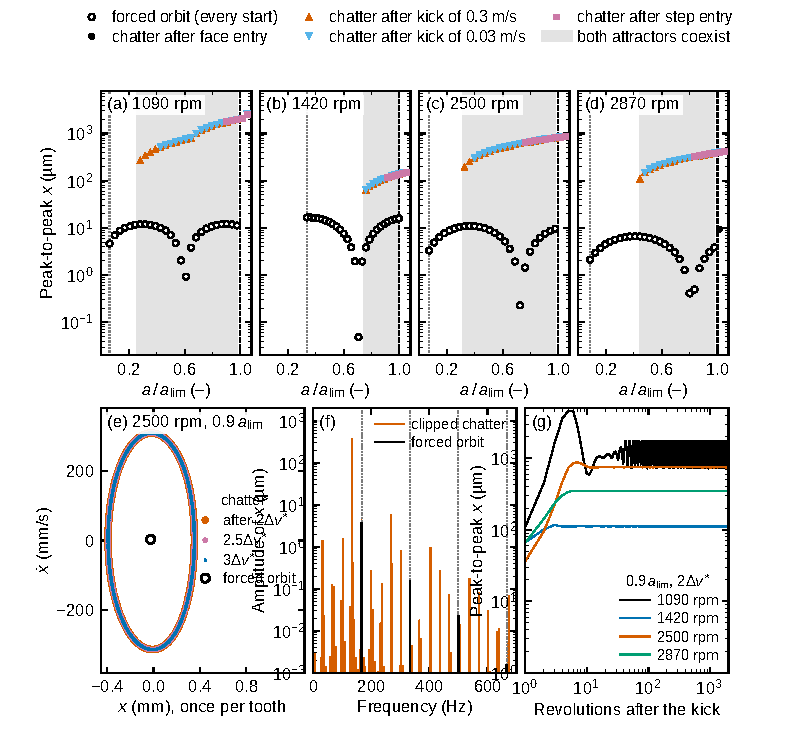
\includegraphics[width=\textwidth]{figures/fig_attractors.pdf}
  \caption{What lies beyond the basin ($g=\SI{1500}{\volt\second\per\metre}$, $\lvert V\rvert\le\SI{9}{\volt}$, full surface memory). (a)--(d)~Steady peak-to-peak displacement over the last 300 of 1600 revolutions against $a/\alim$, for four starts: open circles, the forced orbit, which every start reaches where it is the only attractor; filled markers, bounded chatter. Shaded: both attractors coexist; dotted: $\alim(0)$; dashed: $\alim$. (e)~Once-per-tooth samples of $(x,\dot x)$ of the last 500 tooth periods after kicks of 2, 2.5 and 3 times the critical kick, at \SI{2500}{\rpm} and $0.9\alim$: the three runs settle on the same closed curve around the forced orbit. (f)~Amplitude spectra of $x$ over 500 revolutions at the same point; dotted: tooth-passing harmonics. (g)~Peak-to-peak displacement per revolution after a kick of twice the critical kick at $0.9\alim$.}
  \label{fig:attr}
\end{figure}

\subsection{Describing-function prediction: further remarks}\label{supp:std-bistab-df}

The size of the basin near the limit can be predicted with a dual-input describing function \citep{gelb1968describing} (Section~\ref{M-sec:bistab-df}); \citet{ozsoy2025frequency} predicted the saturation of the settled cut in the frequency domain from its forced response, which is the forced command of Section~\ref{M-sec:model-orbit} (Section~\ref{M-sec:model-second}); their model has no threshold amplitude for disturbances.
A kick $\Delta v$ excites the chatter mode with a velocity amplitude $p\,\Delta v$, where $p$ was fitted on the unclipped cut from the decay of its least-damped mode after a small kick (Section~\ref{supp:bistab-df}).
In Eq.~\eqref{M-eq:dfbasin}, the limit holds because $g_e\to g$ and $\mathcal N(A)=1$ as long as $\bmax+A\le\Vmax$.
% src: src/c1_unsafe_zone.py (df_gain: 128 phases, b on 128 samples per tooth period; critical_amplitude; effective_gain_needed; _mode_factor: kick of 1 mm/s at phase 0, high-pass 40 Hz, fit of the slowest decaying mode)

Where $p$ could be fitted, from 0.7--$0.8\alim$ upwards, the simulated critical kick (median over the phases) is 0.61--1.13 times this estimate, and 0.88--1.13 times at 0.95 and $0.98\alim$ (Fig.~\ref{M-fig:basin}). Equation~\eqref{M-eq:dfbasin} predicts, without proving it, that the basin does not close at the limit but tends to a finite size set by the residual authority $\Vmax-\bmax$, which at $\alim$ is 3.9, 1.7, 0.87 and \SI{4.7}{\volt} at 1090, 1420, 2500 and \SI{2870}{\rpm}; at $0.999\alim$ the simulated critical kick is still 1.4--\SI{10.5}{\milli\metre\per\second} at the three speeds tested (Section~\ref{supp:bistab-basin}). The basin would close below $\alim$ only where $\bmax$ reached $\Vmax$, as it does at some depth below $\kappa\alim$ at the 94 speeds (1530--\SI{2460}{\rpm}) where the steady demand of Section~\ref{M-sec:feasibility} binds; persistent forcing that adds to $b$, such as runout, consumes the residual authority (Section~\ref{M-sec:delayed-robust}). The estimate is cheap, but it rests on the filtering hypothesis and on the factor $p$, fitted at one kick phase and valid only near the limit; $A^*$ is the harmonic-balance amplitude of the unstable limit cycle that bounds the basin.
% src: results/c1_df.npz (A_dual at a = a_lim: 3.92, 1.66, 0.87, 4.69 V at 1090, 1420, 2500, 2870 rpm = V_max - b_max; the 1420 rpm value was 0.009 V before a round-off fix in c1_unsafe_zone.critical_amplitude, tests/test_c1_results.py), results/c1_basin.npz (p_mode finite at frac >= 0.7, at 1420 rpm >= 0.8), results/c1_summary.json (td_over_df 0.61-1.13); ratios at 0.95/0.98 recomputed with the c1_summary formula: 0.88-1.13; verification/tdsim/check11_kick_near_limit.json (1.405-1.467, 7.055-7.611, 9.150-10.533 mm/s); README §11.5; verification/paper/revision_runs.json (closed_form.runout_to_clip_g1500: 0.730, 3.09, 8.74 um at 2500, 2870, 1420 rpm; 1090 rpm below 9 V up to 10 um; worst command over 40 depths up to 0.9 a_lim and 8 runout phases, c4_robust.worst_orbit_command)

\subsection{Checks of the protocols: summary}\label{supp:std-bistab-checks}

The protocols of Section~\ref{M-sec:bistability} were checked against their weak points (Section~\ref{supp:bistab-checks}). At $0.98\,\alim$, kicking at revolution 300 instead of 100 changes the critical kick at one of four phases per speed, by \SI{1.1}{\percent} (one bisection step), and the minimum over these phases at none; judging over 900 instead of 300 revolutions after the kick and using 64 instead of 16 kick phases change the worst-phase critical kick at the four speeds by at most \SI{1.1}{\percent}; the face entry leaves at revolution 100 a deviation from the forced orbit three orders of magnitude below the smallest critical kick. A scan of the band in steps of $0.05\,\alim$ at nine speeds, with the kicks of the band map, finds the lowest chattering depth next to the bisected edge at all nine and no chatter below it. At eight speeds the chattering depths form one interval up to $0.98\,\alim$; at \SI{520}{\rpm} they do not: kicks end in chatter at 0.30--$0.55\,\alim$ and at 0.95--$0.98\,\alim$, but at no grid depth in between. The mapped edge is therefore the lowest depth at which a kick of the protocol tips the cut, and the band above it need not be unsafe throughout.
% src: verification/paper/protocol_phases.json (summary: n_phases_available 64 at all four speeds; min over 64 phases against 16 at 0.98 a_lim: rel_change_of_min -0.0108 at 1090 rpm, 0 at 1420, 2500, 2870 rpm; all.largest_drop_of_min -0.0108); verification/paper/protocol_window.json (summary: 4 points, 53 runs, n_disagreeing_runs 0, ratio 1.0 at 1090/1420/2500/2870 rpm); verification/paper/protocol_kick_timing.json (units.residual_*: dev_x_from_orbit_um at rev100 <= 0.00085, dev_v_from_orbit_mmps <= 0.00073; summary.all: 16 points, ratio 0.989-1, max_abs_rel_change 0.0108; per speed ratio_of_minima 1.0; reproduction_all_identical true); verification/paper/protocol_band_holes.json (summary.all: speeds_complete 9, speeds_with_holes [520], speeds_with_chatter_below_edge [], total_runs 2028; summary.520: chatter_fracs 0.30-0.55, 0.95, 0.98, holes_above_edge 0.60-0.90; grid_edge_frac next to stored_edge_frac at all nine speeds)

\section{Supplement to Section 5: certificates}\label{supp:cert}

This section gives the details of the certificates of Section~\ref{M-sec:certificates} that are not needed to follow the argument: the vertex conditions and the enclosure of the periodic certificate C3, the validation protocols, the effect of the validity bound, what C3 gains over the averaged certificate C2 and how it converges in the number of segments, the results at low radial immersion and the straight-tooth counterexample to averaging.

\subsection{Circle criterion}\label{supp:circle}

The condition of Proposition~\ref{M-prop:circle} was evaluated on a frequency grid of \SI{0.01}{\hertz} over 0.1--\SI{60}{\hertz}, \SI{0.002}{\hertz} over 60--\SI{600}{\hertz} and \SI{0.5}{\hertz} over 600--\SI{5000}{\hertz}, above which $\lvert L\rvert<0.02$. Near $\alim(0)$ the dip of $\operatorname{Re}[1+L(i\omega)]$ is as narrow as the decay rate of the critical root, so the minimum was refined around the eight lowest local minima of $\operatorname{Re}[1+L]$ and the eight highest local maxima of $\lvert L\rvert$ on the grid by three nested zooms of 2001 points each; at 12 test points (four speeds, three depths up to $0.99\alim(0)$) the refinement changed $\mu$ by less than $10^{-5}$ (by at most $2\times10^{-7}$ except at one failing point, $7\times10^{-6}$). The depth $a_{\mathrm{circ}}$ was found by a scan of 39 depths spaced $\alim(0)/40$ followed by bisection to a relative $10^{-6}$. At no speed did a depth pass after a failing one, consistent with the set of depths at which the condition holds being an interval, which at two speeds extends to $\alim(0)$ itself. The condition fails at 124--\SI{196}{\hertz} (median \SI{132}{\hertz}), near the chatter frequency of the uncontrolled cut, whose critical root approaches the imaginary axis; where $a_{\mathrm{circ}}$ is smallest it fails at 124--\SI{129}{\hertz}, near the structural mode. The forced orbit was checked on 2000 depths up to $a_{\mathrm{circ}}$; where the scheduled gain brings the steady command to the clip, Eq.~\eqref{M-eq:feas} holding with equality, a check on 400 depths finds it above \SI{9}{\volt} by at most \SI{5}{\milli\volt}, and the first depth at which it exceeds \SI{9}{\volt} on the 2000-depth grid bounds $a_{\mathrm{circ}}$. With $g=\SI{1500}{\volt\second\per\metre}$ at every speed instead of the scheduled gains, the condition alone holds up to a median over the speeds of $0.954\,\alim(0)$, but the forced orbit is clipped below that depth at 57 speeds (1530--\SI{2090}{\rpm}), down to $0.07\,\alim(0)$ at \SI{1950}{\rpm}.

At the four speeds of Section~\ref{M-sec:bistab-basin}, the depth up to which the frequency condition holds falls slowly with the gain, from 0.986 at $g=\SI{250}{\volt\second\per\metre}$ to $0.862\,\alim(0)$ at $g=\SI{3000}{\volt\second\per\metre}$ at \SI{1420}{\rpm}, and by at most \SI{2}{\percent} over the same range at 1090, 2500 and \SI{2870}{\rpm}. At \SI{1420}{\rpm} the forced orbit itself reaches the clip below that depth for $g\ge\SI{2000}{\volt\second\per\metre}$, so that $a_{\mathrm{circ}}$ is 0.89 and $0.40\,\alim(0)$ at $g=2000$ and 3000; at the other three speeds the orbit stays unclipped. The lower edge of the unsafe band lies above $a_{\mathrm{circ}}$ at all 109 speeds where it was found, by a factor of at least 1.11. The criterion admits any time variation of the sector gain $\varphi(t,y)/y$ in $[0,1]$, whereas in the clipped loop it varies only through $b(t)$ and the deviation itself; this is the source of its conservatism where it fails well below $\alim(0)$. The Popov criterion, which would use more of the structure, requires a time-invariant nonlinearity and does not apply while $b(t)\neq0$.
% src: verification/paper/circle_criterion.py (F_HZ grid, mu, _zoom, a_circ, first_clipped_depth, add_orbit_limit), circle_criterion.json (g_best: orbit_peak_V_up_to_a_circ - 9 V <= 0.0046 V; g1500: ratio_median 0.9537, n_orbit_limited 57, rpm 1530-2090, ratio_eff_min 0.0724 at 1950 rpm; refinement_check: |mu_grid - mu_refined| <= 1.8e-7 at 11 points, 7.2e-6 at 1090 rpm 1.25 mm (failing); g_best: n_nonmonotone 0, n_reached_a0 2; verification/paper/circle_gainsweep_orbit.py/.json (f_fail: 123.7-195.5 Hz, median 131.7; gain_sweep ratio_eff at 1420 rpm 0.889 (g 2000), 0.402 (g 3000), unchanged elsewhere); gain_sweep: 1420 rpm 0.9856 at g = 250 to 0.8617 at g = 3000; 1090 rpm 0.9978-0.9780, 2500 rpm 0.9991-0.9898, 2870 rpm 0.99996-0.99951; band: edge_over_a_circ_min 1.1085, all_edges_above_a_circ true)

\paragraph{Proof on the continuous frequency axis} The proof was made at the scheduled gains of Section~\ref{M-sec:feasibility} (the results for $g=\SI{1500}{\volt\second\per\metre}$ and the gain sweep above rest on the grid). Let $a_\mu$ be the depth found by the bisection above, up to which the frequency condition holds; $a_\mu=a_{\mathrm{circ}}$ except at the 44 speeds where the forced orbit reaches the clip first, where $a_\mu$ is 1.14--4.6 times $a_{\mathrm{circ}}$. With $s=i\omega$, $L=h/B$ with $h=-igK_a\omega^3/A$, $A=\omega_a^2-\omega^2+i\,2\zeta_a\omega_a\omega$ and $B=k-m\omega^2+ic\omega-\overline{aH}\,(1-\cos\omega T+i\sin\omega T)$, so that $\operatorname{Re}[1+L]=\mathcal N/\lvert B\rvert^2$ with $\mathcal N=\lvert B+h/2\rvert^2-\lvert h\rvert^2/4$; $\mathcal N>0$ on a box proves $\operatorname{Re}[1+L]>0$ there and $B\neq0$. This quantity was enclosed on boxes $[\omega_1,\omega_2]\times[a_1,a_2]$ by interval arithmetic in double precision: every addition, multiplication and division rounded outwards by one unit in the last place, cosine and sine bounded by their values at the ends of the interval, padded by $2^{-50}$, and by $\pm1$ wherever an extremum may lie inside, and the model constants taken as intervals of relative half-width $10^{-12}$; a self-test at start-up checks the enclosures against the floating-point $L$ and the cosine and sine used against the C library. Starting from frequency intervals of at most \SI{0.25}{\radian} of $\omega T$ over $[0,2\pi\cdot5000]$\,rad/s, each with the whole depth range $[0,(1-10^{-3})\,a_\mu]$, boxes with a non-positive lower bound were bisected, in frequency or in depth, until every box had a positive lower bound (785--5500 box evaluations per speed; no undecided box at any of the 251 speeds); boxes whose bound was below 0.99 times the grid value of $\mu$, or of $\operatorname{Re}[1+L]$ at the box centre, were then bisected further, for 1200--30\,000 evaluations per speed in all. For $\omega\ge2\pi\cdot\SI{5000}{\radian\per\second}$, $\lvert A\rvert\ge\omega^2-\omega_a^2$ and $\lvert B\rvert\ge m\omega^2-k-2\lvert\overline{aH}\rvert$ give a bound on $\lvert L\rvert$ that decreases with $\omega$ and is at most 0.0071. After the tightening, the smallest certified lower bound of $\operatorname{Re}[1+L]$ over a speed's boxes is 0.00098 at the hardest speed (\SI{950}{\rpm}) and 0.043 at the median one. Because $B\neq0$ on the whole axis for every depth up to $(1-10^{-3})\,a_\mu$ and the cut is stable at $a=0$, the proof also shows that these depths lie below $\alim(0)$. At the smaller of $(1+10^{-3})\,a_\mu$ and the midpoint between $a_\mu$ and $\alim(0)$, the enclosure at the grid minimiser has a negative upper bound at 249 speeds, so the depth at which the frequency condition stops holding is located to within $10^{-3}$; at 2990 and \SI{3000}{\rpm} the condition holds up to $\alim(0)$. The proof covers the averaged model with the constants of the code and relies on the documented error of the C library's cosine and sine; the second hypothesis of Proposition~\ref{M-prop:circle}, an unclipped forced orbit, rests on the closed-form command on 2000 depths, and at the 44 speeds where it fails first it sets $a_{\mathrm{circ}}$.
% src: verification/paper/circle_interval.py (docstring: algebra, intervals, phases, tail, fail check), circle_interval.json, circle_interval.log (251 verified, undecided 0; boxes 1210-29721 per speed; min_lb min 9.8e-4, median 0.0434; tail 7.06e-3; fail check confirmed 249, n/a 2 at 2990 and 3000 rpm); rows: n_box_evals_phase1 785-5454, n_box_evals 1210-29721, min_lb_phase1 min 2.8e-7, min_lb (after tightening) min 9.8e-4 at 950 rpm; a_v_mm = 0.999 a_circ_mm (condition-only depth, circle_criterion.json g_best a_circ_mm), which exceeds a_circ_eff_mm at the 44 orbit-limited speeds 1530-1990 rpm by 1.14-4.57 times; fail point a_f = min(1.001 a_circ_mm, (a_circ_mm + a0)/2); circle_criterion.py: max_orbit_peak_V_up_to_a_circ 9.00463 V from orbit_peak_V_up_to (400 depths), first_clipped_depth on 2000 depths

\subsection{Loss of contact as a second sector condition}\label{supp:contact}

On the engaged arc of half-immersion down milling, $\phi\in[\pi/2,\pi]$, the chip of a slice is $h=f_z\sin\phi+r\lvert\cos\phi\rvert$ with $r=\tilde x-\tilde x(t-T)$ [Eq.~\eqref{M-eq:chip}], so loss of contact occurs only for $r<0$, where $f_z\sin\phi<\lvert r\rvert\lvert\cos\phi\rvert$. The force lost by a slice, $(K_{tc}\sin\phi+K_{rc}\lvert\cos\phi\rvert)\max\{\lvert\cos\phi\rvert\lvert r\rvert-f_z\sin\phi,0\}$, has the sign of the linear regenerative force and is convex in $\lvert r\rvert$, so its ratio to $\lvert\overline{aH}\,r\rvert$ grows with $\lvert r\rvert$ and is largest at $\lvert r\rvert=\delta f_z$. Its largest value over the tooth period, with the helix ($2^{18}$ instants, quadrature error of about $1.3\times10^{-4}$), is $\theta(a,\delta)$: 0.14--0.60 over the 48 depths of Section~\ref{M-sec:cert-c2} at $\delta=0.5$ (largest at shallow depths, where few slices are engaged), 0.17--0.23 at the 12 points of Section~\ref{M-sec:cert-lmi}; its average over the arc is 0.139.

With $\theta=0$ the extended conditions reproduce C2: they give 3.0579 against \SI{3.0578}{\milli\metre\per\second} at \SI{2500}{\rpm} and $0.9\alim$, and the blocks agree bit for bit. Perturbed candidates (multiplier $S_2$ scaled by $10^{\pm3}$ or negative, $\theta$ tripled, the sign of the new column reversed) are rejected by the check. Runs of the collocation model from boundary points of a certified ellipsoid, with the true dead zone and the true lost force, stayed inside it (largest $\mathcal V=0.998$). At $0.9\alim$, with the arc-averaged share 0.139 instead of $\theta$, the certified kick would be 0.89--\SI{0.95}{} times that without loss of contact; with $\delta=1$, where $\theta$ is 0.35--0.40, no certificate exists at \SI{1090}{\rpm} and only a vanishing one (\SI{0.005}{\milli\metre\per\second}) at \SI{2500}{\rpm}, so the larger validity bound does not pay once loss of contact is included.
% src: verification/paper/contact_sector.py/.json (theta: n_tgrid 262144, quadrature_check max rel err 1.3e-4, theta_05_range_48 0.140-0.604, theta_bar_05 0.1394; tests.theta0_reproduction 3.0579046/3.0577848 mm/s, blocks bitwise identical; negative tests rejected; sampled run max_V 0.998; campaign.tradeoff_090: beta2 with theta_bar 5.526/3.543/2.870/6.538 against beta1 6.196/3.843/3.058/6.892 mm/s; delta 1: theta 0.399/0.400/0.391/0.347, beta2 0/2.881/0.005/5.969)

\subsection{Proof of the periodic certificate and details of the C2 results}\label{supp:proof-c3}

\paragraph{Proof of Proposition~\ref{prop:c3}} As $\mathcal A(t)W(t)$ contains $s$, $s^2$ and $rs$, the matrix of Eq.~\eqref{eq:lmi-per}, with $\sigma$ for $s^2$, is affine in $(s,\sigma)$ for fixed $r$ and in $r$ for fixed $(s,\sigma)$; since $(s,s^2)$, $s\in[0,1]$, lies in the triangle spanned by the three points, its value at any $t$ of the segment is a convex combination of the six vertex values. Equations~\eqref{M-eq:lmi-incl}--\eqref{M-eq:lmi-size} are affine in $(W,Y)$, so they hold on segment $k$ with the level $u_{0,k}\le\Vmax-\lvert b(t)\rvert$. The proof of Proposition~\ref{M-prop:c2} then applies on each segment, $\Delta_kW$ accounting for the variation of $W$, and $\mathcal V$ is continuous across the nodes.


\paragraph{Step entry and gain map} The step entry is certified only at $0.3\alim$ at 1090, 1420 and \SI{2870}{\rpm} ($\beta=1.04$--1.61), never at \SI{2500}{\rpm}, and always below the simulated step-entry limits (0.75--$0.90\alim$); at 0.5--$0.9\alim$, $\beta=0.16$--0.72, so no productive depth is certified. Over the gain map of Section~\ref{M-sec:feasibility} (42 speeds, seven depths from 0.5 to $0.98\alim$), 287 of 294 points were certified, with certified kicks of 0--\SI{16}{\milli\metre\per\second} (median 6.6) at $0.9\alim$; the other seven lie at 1520--\SI{2000}{\rpm}, where the gain sits at or near the authority limit and the forced orbit itself saturates ($u_0\le0$, three points) or leaves $u_0=0.04$--\SI{0.38}{\volt}, too little for any candidate to pass the check (Fig.~\ref{fig:surf}).
% src: README §12.5, §12.6; results/c2_step.npz, c2_summary.json (step: td_step_limit_frac 0.895/0.893/0.754/0.821), c3_summary.json (errata.c2_step); results/c2_surface.npz (cert, u0, msg), c2_summary.json (surface), c3_summary.json (errata.c2_surface: 0-16.02, median 6.58)

\subsection{Vertex conditions and enclosure of the periodic certificate}\label{supp:cert-vertex}

On segment $k$, with $W(s)$ and $Y(s)$ from Eq.~\eqref{eq:Wt}, the decrease condition~\eqref{eq:lmi-per} is imposed at the six vertices of Proposition~\ref{prop:c3}, $(s,\sigma)=(0,0)$, $(\tfrac12,0)$ or $(1,1)$ and $r=\pm\varepsilon_k$, as
\begin{equation}\label{eq:app-per}
\begin{bmatrix}\Delta_kW-\Lambda-\Lambda^\top-2\lambda W(s) & BS_k-Y(s)^\top\\ S_kB^\top-Y(s) & 2S_k\end{bmatrix}\succ0,
\end{equation}
where $\Lambda=(A_0+Bk^\top)\,W(s)+E_r\,\big[\nu_0W_k+\nu_1W_{k+1}\big]$, $\nu_0=(c_{0,k}+r)(1-s)+c_{1,k}(s-\sigma)$ and $\nu_1=(c_{0,k}+r)s+c_{1,k}\sigma$; these reproduce $aH(t)W(t)$ exactly when $\sigma=s^2$. Since $E_r=p_rq_r^\top$, with $p_r=e_2/m$ and $q_r=e_1-e_{4+N}$, has rank one, the part of the matrix of Eq.~\eqref{eq:app-per} that depends on $r$ is $-r(\bar p\bar v^\top+\bar v\bar p^\top)$, with $\bar p=[p_r^\top\ 0]^\top$ and $\bar v=[(W(s)q_r)^\top\ 0]^\top$. By Petersen's lemma, exact for a scalar uncertainty \citep{petersen1987stabilization}, the matrix is positive definite for all $\lvert r\rvert\le\varepsilon_k$ if and only if, for some $\varkappa>0$,
\begin{equation}\label{eq:app-merged}
\begin{bmatrix}M_0-\varkappa\bar p\bar p^\top & \varepsilon_k\bar v\\ \varepsilon_k\bar v^\top & \varkappa\end{bmatrix}\succ0,
\end{equation}
with $M_0$ the matrix at $r=0$. Condition~\eqref{eq:app-merged} merges the vertices $r=\pm\varepsilon_k$ and leaves three LMIs per segment; for balance, $p_r$ is divided and $q_r$ multiplied by $10\,\big(\lVert p_r\rVert/(\lVert q_r\rVert\varepsilon_k)\big)^{1/2}$. The independent check tests the six vertices separately, with a round-off scale that also includes $\big(\lVert A_0+Bk^\top\rVert+(\lvert\nu_0\rvert+\lvert\nu_1\rvert)\lVert E_r\rVert\big)\max(\lVert W_k\rVert,\lVert W_{k+1}\rVert)$ and $(\lVert W_k\rVert+\lVert W_{k+1}\rVert)/\tau_s$, to cover rounding in $\Delta_kW$ and in $\mathcal AW$.

The line $c_{0,k}+c_{1,k}s$ is fitted by least squares to $aH$ at the midpoints of 2048 equal cells of segment $k$, and $\varepsilon_k$ is the largest residual plus $(\Upsilon+\lvert c_{1,k}\rvert/\tau_s)\,\tau_s/4096$, where $\Upsilon\ge\lvert\mathrm d(aH)/\mathrm dt\rvert$ holds because each tooth contributes to $\mathrm d(aH)/\mathrm dt$ only through the two ends of its engaged interval in $z$.
% src: src/c3_periodic.py (enclosure: N_ENC 2048; aH_rate_bound; corners; lmi: merged block, P_SCALE 10; check); README §14.2, §14.9

\subsection{Certified kick over the gain map}\label{supp:cert-surface}

Figure~\ref{fig:surf} shows the certified kick of the averaged model over the gain map of Section~\ref{M-sec:feasibility} and the step-entry certificate at the four speeds of Section~\ref{M-sec:cert-c2}.

\begin{figure}[!htbp]
\centering
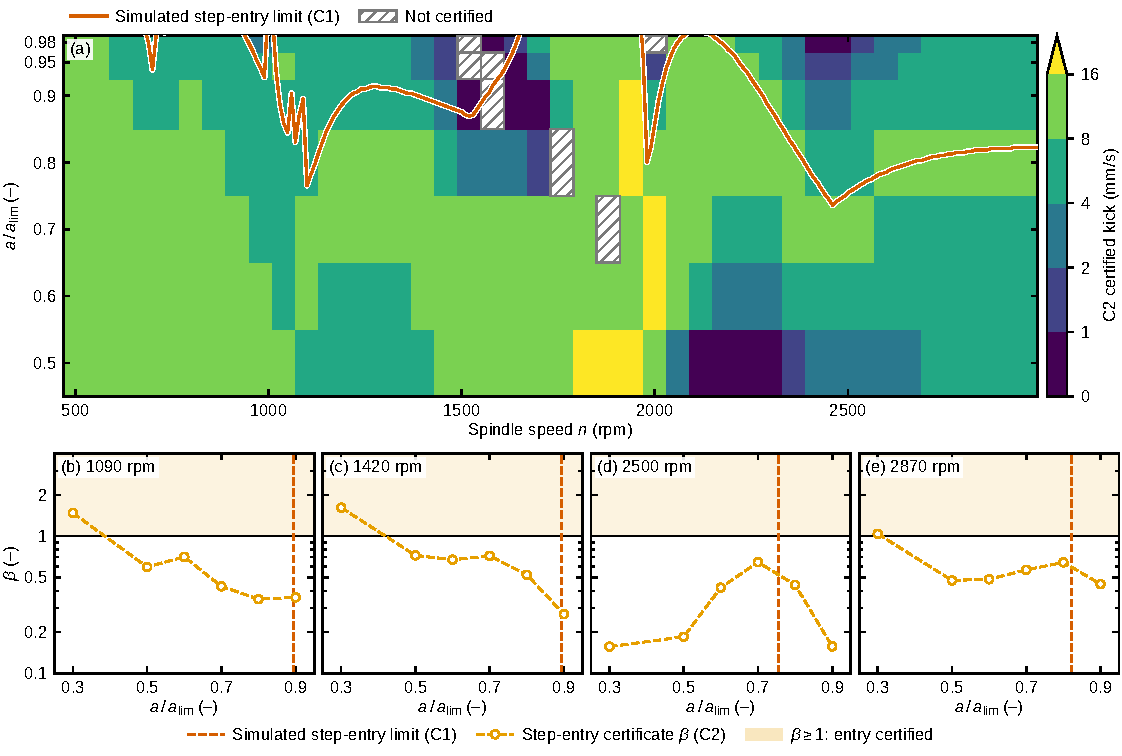
\includegraphics[width=\textwidth]{figures/fig07_certified_surface.pdf}
\caption{(a) Certified kick of the averaged model (C2) over spindle speed and depth on the gain map of Section~\ref{M-sec:feasibility}: 42 speeds and the seven computed depths 0.5, 0.6, 0.7, 0.8, 0.9, 0.95 and $0.98\alim$, drawn as rows of equal height (the vertical axis is not to scale in $a/\alim$), with colour bins in a 1--2--5 sequence. Not certified (7 of 294 points): cross-hatched, the forced orbit itself reaches the clip ($u_0\le0$, three points); hatched, no candidate passed the check (four points). Open circles: depths above the simulated step-entry limit of Section~\ref{M-sec:bistability}, at which the step entry from rest ends in chatter. (b)--(e) Step-entry certificate $\beta$ at the four speeds of Fig.~\ref{M-fig:cert}; $\beta\ge1$ (shaded) certifies the entry at rest on a fresh surface at the entry phase of the simulator; dashed: simulated step-entry limit. Command bound corrected as in Section~\ref{M-sec:cert-lmi}.}
\label{fig:surf}
\end{figure}

\subsection{Validation protocols}\label{supp:cert-protocol}

The off-axis test used boundary points of the certified ellipsoid (for C3, of the ellipsoid at the phase of application) in 18 directions: both signs of the points that maximise $\tilde x$, $\dot{\tilde x}$, $\tilde q$, $\dot{\tilde q}$, $\tilde x(t-T)$ and $\tilde x-\tilde x(t-T)$ on it, and six random points. They were applied in the simulator as full-state deviations at four phases a quarter of a tooth period apart, with the protocol of Section~\ref{app:lmi}. These directions were sampled, not searched for the worst case.

The sampled check followed 48 trajectories per point of the collocated model with the true dead zone over 40 tooth periods, started at 0.999 of the boundary in random directions and phases. $\mathcal V$ never exceeded its initial value 0.998 for C2 and stayed below 0.997 after the first step for C3 (2256 starts). This is only a consistency check, as ellipsoids that are too large can pass it; the certificates rest on the independent check of Section~\ref{M-sec:cert-check}.

Floquet limits of the periodic collocated model used 200 Magnus steps per period and bisection to a relative $10^{-5}$. With $N+8$ nodes the spectral radius at the computed limit differs from 1 by at most $6\times10^{-6}$, and at nine speeds at half immersion the limit agrees with stored semi-discretisation limits \citep{insperger2002semi,insperger2004updated} within $1.3\times10^{-5}$; no such check was made at $a_e/D=0.1$.
% src: src/c2_certificate.py (boundary_directions, deviation_to_pert, td_offaxis, proof_check: nruns 48, nper 40); src/c3_periodic.py (td_offaxis, floquet_a_lim); results/c2_validate.npz (proof_vmax 0.998001, offaxis 0/3456); results/c3_summary.json (basin: proof_starts 2256, proof_vmax 0.9969, offaxis 0/3384); results/c3_floquet.npz (rho_n8: 4.9e-6, 5.5e-6); README §14.4 (SDM agreement 1.3e-5 at nine speeds)

\subsection{Validity bound}\label{supp:cert-delta}

Without the validity bound~\eqref{M-eq:lmi-valid}, the certified ellipsoid at \SI{2500}{\rpm} and $0.7\alim$ admitted histories displaced by 7--12 feeds, with the tool entirely out of the cut. These states return to the orbit in the linear model, but 32 of 72 off-axis runs from its boundary ended in chatter in the simulator, against none with the bound. Table~\ref{tab:delta} gives the certified kick for other values of $\delta$ and without the bound, with the command bound of the original C2 solves. Near the limit the sector condition sets the certificate and $\delta$ hardly matters; at shallow depths the bound sets it, and without the bound $\beta$ doubles at \SI{1090}{\rpm} and $0.15\alim$, but the set may then contain states with the tool out of the cut, as above.
% src: README §12.4 (7-12 f_z; 32 of 72 runs, 0 of 72 with the bound); verification/paper/revision_runs.json (beta_vs_delta; 23.367/11.689 = 2.0 at 1090 rpm, 0.15 a_lim; delta = 0.5 values equal results/c2_validate.npz cert)

\begin{table}[!tbp]
\centering
\caption{Certified kick $\beta$ (\si{\milli\metre\per\second}) of the averaged model (C2) against the validity bound $\delta$ of Eq.~\eqref{M-eq:lmi-valid}; $\delta=0.5$ is used in the article.}
\label{tab:delta}
\small
\begin{tabular}{@{}lcccc@{}}
\toprule
Point & $\delta=0.25$ & $\delta=0.5$ & $\delta=1$ & no bound\\
\midrule
\SI{1090}{\rpm}, $0.15\alim$ & 6.57 & 11.7 & 18.5 & 23.4\\
\SI{2870}{\rpm}, $0.3\alim$ & 5.69 & 8.74 & 10.0 & 10.4\\
\SI{2500}{\rpm}, $0.9\alim$ & 2.90 & 3.06 & 3.07 & 3.07\\
\bottomrule
\end{tabular}
\end{table}
% src: verification/paper/revision_runs.json (beta_vs_delta: 6.5748/11.6891/18.4958/23.3672; 5.6854/8.7429/10.0125/10.3694; 2.8990/3.0579/3.0712/3.0731 mm/s)

\subsection{What the periodic certificate gains, and its convergence}\label{supp:cert-decomp}

At $0.9\alim$ and the four speeds, relative to C2, the periodic coefficient with the single level of C2 gives 0.94--0.98, the averaged model with the segment levels 1.06--1.15, and both together (C3) 1.02--1.12: the periodic coefficient costs 2--6\,\%, and the segment levels gain 6--15\,\%. For the averaged, time-invariant model with a single level, a periodic $W$ cannot gain: the LMIs are then linear in $(W,Y,S)$ with constant coefficients and $\dot W$ integrates to zero over the period, so the period average of a feasible periodic certificate is a feasible constant one of the same size; on the periodic model the argument fails, since the period average of $aH(t)W(t)$ is not the product of the averages. C3 is not converged in the number of segments $M$: relative to C2, $M=8$ gives 0.93--1.03 and $M=32$ gives 1.08--1.22 at $0.9\alim$ (3--12\,\% above $M=16$), at about twice the memory. At $0.98\alim$, $M=32$ gives 5.15, 2.31 and \SI{5.01}{\milli\metre\per\second} at 1090, 1420 and \SI{2870}{\rpm}, against 4.84, 2.08 and \SI{4.83}{\milli\metre\per\second} for C2 and 4.60, 2.05 and \SI{1.70}{\milli\metre\per\second} for $M=16$. At \SI{2500}{\rpm} and $0.98\alim$ no candidate passed with either $M$: the best ones had a positive smallest eigenvalue below the round-off bound.
% src: README §14.5, §14.6; results/c3_decomp.npz, c3_edge.npz, c3_summary.json (decomp: averaged resolved 1.056-1.153, periodic single level 0.939-0.983, m_c 8 0.927-1.034, m_c 16 1.017-1.121, m_c 32 1.077-1.215; edge: c2 4.843/2.081/1.139/4.826, m_c_16 4.601/2.046/0/1.700, m_c_32 5.152/2.313/0/5.013 mm/s)

\subsection{Low radial immersion}\label{supp:cert-lowimm}

At $a_e/D=0.1$, $aH(t)$ varies more: over the four speeds it spans 0.66--1.40 times its mean at $0.5\alim$ and 0.79--1.24 times at $0.9\alim$, against 0.77--1.27 and 0.88--1.11 at half immersion, and the limits are 30--\SI{65}{\milli\metre} (14--\SI{30}{\milli\metre} at half immersion). All eight points (0.5 and $0.9\alim$) were certified, with C3/C2 = 0.94--1.04; the periodic and averaged critical kicks agree within 0.974--1.052, the certificate lies below $\Delta v^*$ in all 16 cases tested (four phases at the four points with finite $\Delta v^*$), and none of the 576 off-axis runs ended in chatter.
% src: README §14.4, §14.7; results/c3_lowimm.npz, c3_summary.json (lowimm: c3_over_c2 0.944-1.039, periodic_over_averaged_model 0.9739-1.0516, phase_cert_below_td 16/16, offaxis 0/576); aH ranges re-evaluated in closed form (0.660-1.403, 0.787-1.241; 0.766-1.272, 0.881-1.109)

\subsection{Straight teeth: a counterexample to averaging}\label{supp:cert-straight}

Averaging is known to fail in strongly interrupted cutting \citep{davies2002stability,bayly2003stability,merdol2004multi}. With straight teeth $aH(t)$ jumps as teeth enter and leave the cut, and at half immersion between 1600 and \SI{2100}{\rpm} (steps of \SI{25}{\rpm}) the uncontrolled cut has flip lobes below the averaged limit at 12 of 21 speeds (1675--\SI{1950}{\rpm}, from 0.947 of that limit). Where they persist with DVF ($g=\SI{100}{\volt\second\per\metre}$ at four speeds; the gain of the map at \SI{1950}{\rpm}), the forced orbit alone needs 27--\SI{66}{\volt} at 0.98 of the averaged limit, so $u_0<0$ and C2 claims nothing; gains of 250 and \SI{500}{\volt\second\per\metre} removed them, while gains of 141--\SI{250}{\volt\second\per\metre} and straight teeth at low immersion were not examined. Without control there is no forced command and the method of C2 does certify, which gives the counterexample of Table~\ref{tab:counter}: the averaged model, and with it the C2 certificate, is the same for both cutters, whereas the periodic model separates them. With straight teeth the cut is linearly unstable, though nearly benign in practice, its period-two oscillation staying at about \SI{1}{\micro\metre}.
% src: README §14.8; results/c3_straight.npz, c3_counter.npz (x_tooth alternation about 0.53 um, i.e. about 1 um peak to peak), c3_summary.json (straight, counter)

\begin{table}[!tbp]
\centering
\caption{Counterexample to averaging: \SI{1850}{\rpm}, no control ($g=0$), depth 0.98 times the averaged limit (\SI{23.6}{\milli\metre}), half immersion.}
\label{tab:counter}
\small
\begin{tabular}{@{}>{\raggedright\arraybackslash}p{0.34\textwidth}>{\raggedright\arraybackslash}p{0.29\textwidth}>{\raggedright\arraybackslash}p{0.27\textwidth}@{}}
\toprule
 & Straight teeth & Helical teeth (\ang{45})\\
\midrule
Critical Floquet multiplier & modulus 1.034 at \ang{180} & modulus 0.977 at \ang{177}\\
C2 certificate (averaged model) & \SI{13.2}{\milli\metre\per\second} & \SI{13.2}{\milli\metre\per\second}\\
C3 certificate (periodic model) & none (linearly unstable) & \SI{13.1}{\milli\metre\per\second}\\
Simulator after a \SI{0.1}{\milli\metre\per\second} kick & never settles; period-two oscillation of about \SI{1}{\micro\metre} & settles\\
\bottomrule
\end{tabular}
\end{table}
% src: README §14.8; results/c3_counter.npz (a 23.63 mm, mu_abs 1.0342/0.9767, mu_arg 180/177 deg, c2_size 13.201, c3_size 0/13.090 mm/s, sim_stable False/True), log_c3_counter.txt

% Material moved from Section 5 of the full version (../sections/s5_certificates.tex) for the standard-length article.
% Input at the end of Section S5. References with the prefix M- point to the article; references without prefix point to this Supplementary Material.
\subsection{Proofs for the basin estimates}\label{supp:std-proofs}

The sector condition in Eq.~\eqref{M-eq:phi-sector} holds because the saturation is nondecreasing and 1-Lipschitz.
\begin{proof}[Proof of Proposition~\ref{M-prop:circle}]
$L$ is the transfer function of an exponentially stable retarded system, so it is bounded and analytic in $\operatorname{Re}s\ge0$. By the circle criterion for a time-varying nonlinearity in the sector $[0,1]$ and a stable linear part, which may be infinite-dimensional \citep{zames1966inputI,zames1966inputII,desoer1975feedback}, the loop is finite-gain $\mathcal L_2$-stable when $\inf_\omega\operatorname{Re}[1+L(i\omega)]>0$. An initial deviation of the state and its history enters the loop as the free response of the linear part, which decays exponentially. Hence $y$ and $\varphi$ are square integrable, and so are $\tilde x$ and its derivatives, which are also bounded; $\tilde x\to0$ follows by Barbalat's lemma \citep{khalil2002nonlinear}.
\end{proof}

Lemma~\ref{M-lem:sector} follows from a sharper statement: at any $t$ with $\lvert b(t)\rvert<\Vmax$ and for all $w,v\in\mathbb R$,
\begin{equation}\label{eq:sector-sharp}
-\Vmax-b(t)\le w-v\le\Vmax-b(t)\quad\Longrightarrow\quad\psi(w,t)\,\big[\psi(w,t)-v\big]\le0 .
\end{equation}
\begin{proof}[Proof of Lemma~\ref{M-lem:sector}]
If $w>\Vmax-b(t)$, then $\psi=w-\Vmax+b(t)>0$ and $\psi-v=(w-v)-\Vmax+b(t)\le0$; if $w<-\Vmax-b(t)$, then $\psi<0$ and $\psi-v=(w-v)+\Vmax+b(t)\ge0$; otherwise $\psi=0$. Equation~\eqref{M-eq:sector} follows, as $\lvert w-v\rvert\le u_0\le\Vmax-\lvert b(t)\rvert$.
\end{proof}

\begin{proof}[Proof of Proposition~\ref{M-prop:c2}]
Let $P=W^{-1}$ and $\Gamma=YP$. By a Schur complement, Eq.~\eqref{M-eq:lmi-incl} reads $(k^\top-\Gamma)W(k^\top-\Gamma)^\top\le u_0^2$, so $\lvert(k^\top-\Gamma)\xi\rvert\le u_0$ on $\mathcal E(P)$, where Lemma~\ref{M-lem:sector} with $w=k^\top\xi$ and $v=\Gamma\xi$ gives $\psi(\psi-\Gamma\xi)\le0$ at every $t$. There, $\dot{\mathcal V}\le2\xi^\top P(\mathcal A\xi-B\psi)-2S^{-1}\psi(\psi-\Gamma\xi)$, a quadratic form in $(\xi,\psi)$ that the congruence with $\operatorname{diag}(W,S)$ turns into minus the matrix of Eq.~\eqref{M-eq:lmi-dec} at $\lambda=0$. Being negative definite, it gives $\dot{\mathcal V}\le-c\,\mathcal V$ for some $c>0$: $\mathcal E(P)$ is forward invariant and $\mathcal V$ decays exponentially. Equations~\eqref{M-eq:lmi-valid} and~\eqref{M-eq:lmi-size} are equivalent to $\lvert\chi\xi\rvert\le\delta f_z$ on $\mathcal E(P)$, where $\chi\xi=x-x(t-T)$, and to $\beta^2e^\top Pe\le1$.
\end{proof}

\subsection{Global attractivity below the uncontrolled limit: frequency condition and range of validity}\label{supp:std-circle}

Let $a_{\mu}(n,g)$ be the largest depth below $\alim(0)$ up to which the condition holds, and $a_{\mathrm{circ}}\le a_\mu$ the largest up to which, in addition, the forced orbit is unclipped. The condition was located on a frequency grid of \SI{0.002}{\hertz} near the structural mode, whose local refinement changed $\mu$ by less than $10^{-5}$ at 12 test points, and then proved on the continuous frequency axis at the scheduled gains: interval arithmetic with outward rounding encloses $\operatorname{Re}[1+L(i\omega)]$ on boxes of frequency and depth, and an adaptive subdivision shows it to be positive for every $\omega\ge0$ and every depth up to $(1-10^{-3})\,a_\mu$ at all 251 speeds, with the analytic bound $\lvert L\rvert\le0.0071$ above \SI{5}{\kilo\hertz}, while the same enclosures show it failing just above $a_\mu$ at the 249 speeds where $a_\mu<\alim(0)$ (Section~\ref{supp:circle}). The second hypothesis, an unclipped forced orbit, rests on the closed-form command on a dense depth grid. At the scheduled gains of Section~\ref{M-sec:feasibility}, the median of $a_{\mathrm{circ}}$ over the speeds is $0.967\,\alim(0)$, and $a_{\mathrm{circ}}$ is at least $0.96\,\alim(0)$ above \SI{2060}{\rpm}. It is smaller where the condition fails near the structural mode, down to 0.37--$0.40\,\alim(0)$ at 650, 970 and \SI{980}{\rpm}, and at the 44 speeds between 1530 and \SI{1990}{\rpm}, where the scheduled gain of Section~\ref{M-sec:feas-res} brings the forced command to the clip at 6.05--\SI{6.31}{\milli\metre} and $a_{\mathrm{circ}}$ is 0.22--$0.80\,\alim(0)$; in all, it lies below $0.9\,\alim(0)$ at 78 of the 251 speeds. Proposition~\ref{M-prop:circle} holds for the delay equation itself, without collocation, but only for the averaged coefficient and the linear force law. For the averaged linear-force model it proves the counterpart of part of what the simulations suggest (Section~\ref{M-sec:bistab-map}), where the edge of the band in which kicks cause chatter lies above $1.08\,\alim(0)$ at every speed where it was found. No global statement can hold above $\alim(0)$, where the uncontrolled cut is exponentially unstable and a bounded input cannot stabilise it globally \citep{hu2001book}; there, only regional estimates are possible.
% src (interval proof): verification/paper/circle_interval.py/.json (251 speeds verified at (1 - 1e-3) a_circ, 0 undecided boxes; tail bound |L| <= 7.06e-3 for f >= 5 kHz; fail check confirmed at 249 speeds, n/a at 2990 and 3000 rpm where a_circ reaches a_lim(0)); circle_interval.log
% src: verification/paper/circle_criterion.json (g_best: ratio_eff_median 0.9667; rows ratio_eff >= 0.963 at 2060-3000 rpm; rows 650/970/980 rpm ratio_eff 0.366/0.392/0.401 (f_fail_hz 124-129); n_orbit_limited 44, rpm_orbit_limited 1530-1990, first_clipped_depth_mm 6.05-6.31, orbit_limited_ratio_eff 0.218-0.798; n_ratio_eff_below_0p9 78; refinement_check: |mu_grid - mu_refined| < 1e-5; band: all_edges_above_a_circ true, edge_over_a0_min 1.084); results/c1_band.npz

\subsection{Deviation dynamics and collocation model: details}\label{supp:std-cert-model}

Let $x_p(t)$ be the $T$-periodic forced orbit of Section~\ref{M-sec:model-orbit} and $b(t)=-g\dot x_p(t)$ its command, with $\lvert b(t)\rvert<\Vmax$, so that the clip is inactive on the orbit. Since $x_p(t)-x_p(t-T)=0$, the regenerative force vanishes on the orbit, and the deviation $\tilde x=x-x_p$ obeys Eq.~\eqref{M-eq:dev}. The history $\tilde x(t+\vartheta)$, $\vartheta\in[-T,0]$, is represented by its values at the Chebyshev nodes $\vartheta_j=-\tfrac T2\big(1-\cos\tfrac{\pi j}{N}\big)$, $j=1,\dots,N$, and its transport equation is collocated with the Chebyshev differentiation matrix \citep{breda2005pseudospectral,breda2015book}, as for the periodic milling equation \citep{butcher2009chebyshev}. In Eq.~\eqref{M-eq:coll}, $e_i$ are the unit vectors. The dead zone~\eqref{M-eq:deadzone} vanishes for $-\Vmax-b(t)\le w\le\Vmax-b(t)$: unlike that of a fixed saturation, it moves with the forced command and is asymmetric whenever $b(t)\neq0$. With $N=16+4\lceil T\omega_n/2\pi\rceil$ nodes (20--32), the rightmost eigenvalues of the averaged collocated model agree with those of the delay equation to $3\times10^{-8}$.
% src: README §12.2; src/c2_certificate.py (model, nodes_for, history_nodes); src/c3_periodic.py (model); tests/test_c2_certificate.py (crossing at a_lim)

The certificates are therefore numerically verified for Eq.~\eqref{M-eq:coll}, the $N$-node collocation of the averaged or the time-periodic model, not for the delay equation or the simulator, and convergence of the eigenvalues in $N$ does not imply convergence of the certified set; Section~\ref{supp:std-levels} examines it.

\subsection{Sector condition, command bound and size directions}\label{supp:std-bound}

Equation~\eqref{M-eq:sector} is the generalised sector condition of \citet{gomesdasilva2005antiwindup} for the moving dead zone; as for non-symmetric saturation or operation around a non-zero input \citep{hu2001book,tarbouriech2011book,hu2002disturbance}, the input already in use, here by the forced orbit, is removed from the level. For an ellipsoid centred on the orbit, Eq.~\eqref{eq:sector-sharp} reduces to $\lvert w-v\rvert\le\Vmax-\lvert b(t)\rvert$ at each $t$: C2 uses its minimum over the period, C3 its minimum over each segment. The bound $\bar b$ is the rigorous one of Section~\ref{app:lmi}; C2, solved with a slightly lower bound, was rescaled to it by factors of 0.997--1.000 at the 48 points of Section~\ref{M-sec:cert-c2} and down to 0.86 on the surface grid.
% src: README §12.2, §14.9; results/c3_summary.json (errata: size_factor 0.9972-0.99995 at the 48 points, 0.858-1 on the surface); src/c3_summary.py (margin_errata)

In the size condition~\eqref{M-eq:lmi-size}, the direction $e$ is chosen as follows. For $e=e_2$, $\beta$ is a certified kick in m/s, since a velocity kick at any phase moves the state to $\Delta v\,e_2$. For $e=-\xi_p(0)$, minus the orbit state at $t=0$ with its history, where a cut that enters at rest on a fresh surface starts, $\beta\ge1$ certifies the step entry at the entry phase of the simulator.

\subsection{Validity bound and loss of contact}\label{supp:std-contact}

The validity bound~\eqref{M-eq:lmi-valid} excludes gross loss of contact: without it, at \SI{2500}{\rpm} and $0.7\alim$, 32 of 72 off-axis perturbations on its boundary ended in chatter in the simulator; with it, none did. The value $\delta=0.5$ is a choice: with $\delta=1$, $\beta$ rises by \SI{58}{\percent} at \SI{1090}{\rpm} and $0.15\alim$ but by only \SI{0.4}{\percent} at \SI{2500}{\rpm} and $0.9\alim$, so the bound limits the certificates at shallow depths and the sector condition near the limit (Section~\ref{supp:cert-delta}, Table~\ref{tab:delta}).
% src: README §12.2, §12.4 (32 of 72 off-axis runs without the bound), §12.7; verification/paper/revision_runs.json (beta_vs_delta, delta = 1 over delta = 0.5: 18.496/11.689 = 1.582 at 1090 rpm 0.15 a_lim, 3.0712/3.0579 = 1.004 at 2500 rpm 0.9 a_lim)

Inside the bound the chip can still vanish near the tool exit, over the last $\arctan\delta\approx\ang{27}$ of the \ang{90} engagement arc. As the rectified chip $\max\{h,0\}$ has slopes in $[0,1]$, this loss of contact is a second sector nonlinearity: on the set $\lvert\tilde x-\tilde x(t-T)\rvert\le\delta f_z$, the regenerative force lost to it is $\psi_2=\eta\,\overline{aH}\,\chi\xi$ with $\eta\in[0,\theta]$, where $\theta(a,\delta)$ is the largest share of the lost force over the tooth period, relative to the mean coefficient (0.17--0.23 at $\delta=0.5$ at the 12 points examined below; 0.14 averaged over the arc). With $\psi_2$ the model becomes $\dot\xi=\mathcal A\xi-B\psi-(e_2/m)\psi_2$, and the inverse $S_2>0$ of a second S-procedure multiplier extends Eq.~\eqref{M-eq:lmi-dec} to
\begin{equation}\label{eq:lmi-dec2}
\begin{bmatrix}-(\mathcal AW+W\mathcal A^\top)-2\lambda W & BS-Y^\top & (e_2/m)S_2-\theta\,\overline{aH}\,W\chi^\top\\ SB^\top-Y & 2S & 0\\ S_2e_2^\top/m-\theta\,\overline{aH}\,\chi W & 0 & 2S_2\end{bmatrix}\succ0 ,
\end{equation}
which certifies the averaged collocation model with the memoryless part of the loss of contact; a tooth cutting an older surface where contact was lost is not covered. At 0.5 and $0.9\alim$ at the four speeds of Section~\ref{M-sec:bistab-basin}, the certified kick falls by 6--\SI{15}{\percent}. At $0.98\alim$ no certificate exists: without the dead-zone row, Eq.~\eqref{eq:lmi-dec2} is the circle criterion of the sector $[0,\theta]$ for the unclipped loop, which by the Kalman--Yakubovich--Popov lemma requires $\theta<\theta_{\mathrm{c}}=1/\max_\omega\bigl(-\operatorname{Re}[L_0/(1-L_0)]\bigr)$, $L_0(i\omega)=\overline{aH}\,(1-e^{-i\omega T})\,G_{\mathrm{cl}}(i\omega)$, and close to the limit $\theta_{\mathrm{c}}=0.05$--0.09 is below $\theta=0.17$--0.21. The sector admits an arbitrarily fast variation of the lost share, which a cut that close to its limit cannot absorb in this worst case. Near the limit the estimates therefore rest on the linear force law of the collocation model, while the simulator, which has the loss of contact, never violated them.
% src: verification/paper/contact_sector.py/.json (theta.theta_bar_05 0.139; campaign.points: theta_05 0.167-0.228; ratio beta2/beta1 at 0.5 a_lim 0.937/0.878/0.937/0.930 and at 0.9 a_lim 0.851/0.877/0.902/0.930 (1090/1420/2500/2870 rpm); at 0.98 a_lim beta2 = 0, theta_circle_dde 0.047/0.089/0.081/0.077 against theta_05 0.170/0.201/0.207/0.215; tests: theta = 0 path reproduces c2.certify_kick to 4e-5 and 2e-3; sampled runs with the true lost force stay inside the ellipsoid)

\subsection{Periodic certificate and independent check}\label{supp:std-periodic}

C3 keeps the periodic coefficient $aH(t)$ and the forced orbit of C2; over the period, $\lvert b(t)\rvert$ ranges from nearly zero to \SI{7.9}{\volt} at \SI{2500}{\rpm} and $0.98\alim$, whereas C2 uses only its peak. The tooth period is divided into $M=16$ segments, on which $W(t)$ and $Y(t)$ are linear in time and $S$ is constant, so that $\mathcal V(t,\xi)=\xi^\top W(t)^{-1}\xi$ is continuous and $T$-periodic. On each segment, $aH(t)$ is enclosed by a line and a residual bound, the decrease condition, convex in the position on the segment once its square is relaxed, is imposed at six vertices, and the sector condition uses the level $u_{0,k}=\Vmax-\bar b_k$ of the segment. Proposition~\ref{prop:c3} of Section~\ref{app:lmi} then gives the conclusions of Proposition~\ref{M-prop:c2} for the tube $\{(t,\xi):\xi^\top W(t)^{-1}\xi\le1\}$; the certified kick valid at every phase is the smallest nodal size. Piecewise-linear Lyapunov matrices and regions of attraction of saturated periodic systems are established \citep{allerhand2011robust,briat2013clock,li2015periodic,zhou2011periodic,yang2015periodic}; only the application is new here.
% src: README §14.1, §14.2; src/c3_periodic.py (aH, orbit, enclosure); |b| range re-evaluated in closed form with c3_periodic.orbit (0.031-7.870 V at 2500 rpm, 0.98 a_lim)

Every candidate $(W,Y,S)$ returned by the interior-point solver Clarabel \citep{goulart2024clarabel}, asked for a decay margin $\lambda>0$, was checked independently at $\lambda=0$, through the smallest eigenvalue of every decrease matrix against a round-off bound and through Cholesky factors of $W$ for the other conditions (Section~\ref{app:lmi}). The hypotheses of Propositions~\ref{M-prop:c2} and~\ref{prop:c3} are thus verified numerically, in floating point rather than by interval arithmetic.
% src: src/c2_certificate.py (scaling, lmi, check, certify); src/c3_periodic.py (check); README §12.3

\subsection{Results on the averaged model (C2): details}\label{supp:std-c2}

C2 was computed at the 48 clipped points of Section~\ref{M-sec:bistability} (four speeds, 12 depths from 0.15 to $0.98\alim$; Fig.~\ref{M-fig:cert}, Table~\ref{tab:cert}). All 48 passed the check, with $\beta=0.96$--\SI{12.9}{\milli\metre\per\second}, or 1.2--\SI{16}{\micro\metre} as an equivalent displacement $\beta/\omega_n$. Wherever the simulated critical kick is finite (29 points), $\beta$ lies below it, by factors $\Delta v^*/\beta$ of 1.5--28 and with a median of 2.3 from $0.7\alim$ upwards; at the other 19 points no kick up to \SI{3}{\metre\per\second} ended in chatter, and the certificates there (1.7--\SI{12.5}{\milli\metre\per\second}) are at least 240 times smaller than the largest kick tested. The critical kick of the averaged collocation model is itself 0.62--0.99 times $\Delta v^*$ (median 0.92), so the gap lies mainly between the certificate and its own model. Boundary points of the ellipsoid in 18 sampled directions, applied in the simulator at four phases, never ended in chatter (3456 runs; Section~\ref{supp:cert-protocol}).
% src: README §12.4; results/c2_validate.npz, c2_summary.json (validate), c3_summary.json (errata.c2_validate: 1.48-27.59, median 2.34 from 0.7 a_lim); results/c2_validate.npz recomputed: td_min infinite at 19 points, cert there 1.672-12.514 mm/s (1.668-12.512 after the errata factors), 3 m/s / cert = 239.8-1798 (240 at 1420 rpm, 0.7 a_lim; 1800 at 2500 rpm, 0.3 a_lim); model/TD 0.620-0.989, median 0.92; offaxis 0/3456

\begin{table}[!tbp]
\centering
\caption{Certificates at the 48 clipped points of Section~\ref{M-sec:bistability} (four speeds, 12 depths from 0.15 to $0.98\alim$, $g=\SI{1500}{\volt\second\per\metre}$): consistency with the collocation model and validation in the simulator. $\Delta v^*$: simulated critical kick; C2 corrected for the command bound.}
\label{tab:cert}
\small
\begin{tabular}{@{}>{\raggedright\arraybackslash}p{0.36\textwidth}>{\raggedright\arraybackslash}p{0.27\textwidth}>{\raggedright\arraybackslash}p{0.27\textwidth}@{}}
\toprule
 & C2 (averaged model) & C3 (periodic model, $M=16$)\\
\midrule
Certificates that passed the check & 48/48 & 47/48\\
Certified kick $\beta$ (\si{\milli\metre\per\second}) & 0.96--12.9 & 1.70--13.0\\
C3/C2 (median) & -- & 0.35--2.0 (1.06)\\
\midrule
\multicolumn{3}{@{}l}{\emph{Consistency with the collocation model}}\\
$\beta$ below the model's critical kick & 44/44 (minimum over 4 phases, bisection to about 2\,\%) & 688/688 (per phase, 43 points, bisection to 0.06\,\%)\\
Sampled check, largest $\mathcal V$ & 0.998 (start value) & 0.997 (after the first step)\\
\midrule
\multicolumn{3}{@{}l}{\emph{Validation in the simulator}}\\
$\beta$ below $\Delta v^*$ & 29/29 (minimum over 16 phases) & 448/448 (per phase, 28 points)\\
$\Delta v^*/\beta$, all points & 1.48--27.6 & 1.46--14.0\\
$\Delta v^*/\beta$ from $0.7\alim$ (median) & 1.48--3.26 (2.34) & 1.46--4.78 (2.27)\\
Model critical kick$/\Delta v^*$ (median) & 0.62--0.99 (0.92) & 0.61--0.98 (0.90)\\
Off-axis runs ending in chatter & 0/3456 & 0/3384\\
\bottomrule
\end{tabular}
\end{table}
% src: results/c2_summary.json, c3_summary.json (basin: cert_mm_s, phase_cert_below_model/td, td_over_cert, td_over_cert_from_07, model_over_td, offaxis, proof_vmax, c3_over_c2; errata.c2_validate); results/c2_validate.npz (C2 beta corrected 0.958-12.889 mm/s, model/TD 0.620-0.989); src/c2_certificate.py (model_critical_kick: nbis 9 on [1e-4, 3] m/s), src/c3_periodic.py (NBIS 14)

The step entry, certified along $-\xi_p(0)$, is certified only at $0.3\alim$ at three of the four speeds, never at productive depths; over the gain map of Section~\ref{M-sec:feasibility}, 287 of 294 points were certified, the other seven having little or no residual authority (Section~\ref{supp:proof-c3}, Fig.~\ref{fig:surf}).
% src: README §12.5; results/c2_step.npz, c2_summary.json (step), c3_summary.json (errata.c2_step: 1.48/1.61/1.04 corrected at 0.3 a_lim; 0.16-0.72 at 0.5-0.9 a_lim); README §12.6; results/c2_surface.npz (287/294; u0 <= 0 at three points, 0.04-0.38 V at four)

\subsection{Results on the periodic model (C3) and comparison with C2}\label{supp:std-c3}

For the linear limit of this cutter averaging is nearly exact: on the gain map the Floquet limit of the periodic collocated model is 1.0000--1.0011 times the averaged limit (up to 1.0028 at $a_e/D=0.1$), without flip lobes, as the helix cancels most of the variation of $aH(t)$ over the one to five axial pitches that the limits span \citep{insperger2006helix,zatarain2006helix}.
% src: README §14.4; results/c3_floquet.npz, c3_summary.json (floquet: 1.0000-1.0011 and 1.0000-1.0028, below_zoa 0, flip 0)

At the 48 points, 47 C3 certificates passed the check. C3 exceeds C2 at 44 of the 47 points, by a median factor of 1.06, most (1.4--2.0) at \SI{2500}{\rpm} and 0.25--$0.5\alim$, where $\lvert b(t)\rvert$ peaks only briefly: the gain comes from the segment levels, while the periodic coefficient itself costs a few per cent. At $0.98\alim$, C3 falls below C2 at the other three speeds (down to 0.35 times at \SI{2870}{\rpm}), although the periodic model is not more fragile there: C3 is not converged in the number of segments, and with 32 segments it exceeds C2 at these points (Section~\ref{supp:cert-decomp}).
% src: README §14.5, §14.6; results/c3_basin.npz (periodic/averaged minimum kick at 0.98 a_lim 1.013/1.027/1.013/1.002), c3_edge.npz, c3_decomp.npz, c3_summary.json (basin: c3_over_c2 0.35-2.0, median 1.06; edge: C3/C2 0.95/0.98/0.35 at 1090/1420/2870 rpm; m_c_32 5.152/2.313/5.013 against C2 4.843/2.081/4.826 mm/s; decomp)

Phase by phase, C3 lies below the simulated and the model critical kicks in all 448 and 688 cases, and no off-axis run ended in chatter (Table~\ref{tab:cert}). The critical kick of the periodic model is 0.97--1.05 times that of the averaged model (704 pairs): the factor of about 2.3 between the certificates and the simulated basin near the limit is not caused by averaging, also at $a_e/D=0.1$ (Section~\ref{supp:cert-lowimm}). For design, C2 is the practical choice.
% src: README §14.5, §14.7, §14.10; results/c3_basin.npz, c3_summary.json (basin: phase_cert_below_td 448/448, phase_cert_below_model 688/688, offaxis 0/3384, td_over_cert_from_07, periodic_over_averaged_model 0.9727-1.0516; lowimm)

Averaging is known to fail in strongly interrupted cutting \citep{davies2002stability,bayly2003stability,merdol2004multi}; a straight-tooth counterexample, in which only the periodic certificate rejects a linearly unstable cut, is in Section~\ref{supp:cert-straight}.

\subsection{What is certified, and for which model}\label{supp:std-levels}

The critical kick $\Delta v^*$ of Section~\ref{M-sec:bistability} samples the basin of the forced orbit along one direction, in a simulator. Section~\ref{M-sec:certificates} bounds the basin from inside, at three levels of modelling that must be kept apart. For the delay equation of the averaged, linear-force model, a frequency-domain condition, proved on the whole frequency axis by interval arithmetic, together with a forced orbit checked in closed form to stay unclipped on a dense depth grid, shows that the forced orbit attracts every solution below a depth whose median over the speeds is 0.97 of the uncontrolled limit (Section~\ref{M-sec:cert-global}). For finite-dimensional collocation models of the averaged (C2) and the time-periodic (C3) delay equation, linear matrix inequalities give ellipsoidal inner estimates of the basin, numerically verified: every trajectory of these models that starts inside returns to the forced orbit despite the clip (Sections~\ref{M-sec:cert-model}--\ref{M-sec:cert-periodic}). The simulator, with the time-periodic force, loss of contact and the surface memory, checks both (Section~\ref{M-sec:cert-c2}). No statement is made here for the physical machine. Unlike regional estimates for chatter controllers designed with input constraints \citep{zhang2015ellipsoid,wu2016adaptive}, the DVF law is fixed and the dead zone of the clip moves with the forced command $b(t)$, so that the authority spent on the forced orbit enters the estimate.

The estimates of Section~\ref{M-sec:certificates} hold at three levels, which the evidence for each keeps apart. For the averaged delay equation with a linear force law, Proposition~\ref{M-prop:circle} is a global result, without collocation, up to $a_{\mathrm{circ}}$, with its frequency condition proved by interval arithmetic and its unclipped forced orbit checked on a dense depth grid. For the finite-dimensional collocation models, the LMIs are numerically verified, and their size depends on the discretisation: doubling the number $N$ of collocation nodes changes the certified kick of C2 by $-5.0$ to $+0.6$\,\% at ten of eleven points, most at \SI{1090}{\rpm} and half the limit (Table~\ref{tab:nconv}). At the eleventh, \SI{2500}{\rpm} and $0.98\,\alim$, where the residual authority is smallest, no candidate of the solve with $2N=40$ nodes passed the independent check, but 24, 30 and 36 nodes change the certified kick by only \SI{0.6}{\percent}, which points to the conditioning of the larger problem rather than to a loss of the certificate. A certificate thus holds for the collocation model for which it was computed, and its size is converged in $N$ to within a few per cent. In the number of segments of C3 the certified size grows from $M=8$ to 16 and 32 (Section~\ref{supp:cert-decomp}); as every $M$ gives a valid certificate, this lack of convergence makes C3 more conservative, not wrong. For the simulator, which has the time-periodic force, loss of contact and the surface memory, every certificate lies below the simulated critical kick, and no perturbation on the boundary of an estimate ended in chatter: 0 of 3456 off-axis runs for C2 and, with C3 solved again at the four speeds at $0.9\,\alim$ and at the three where it exists at $0.98\,\alim$ and its tube applied with the full surface memory instead of the last four passes, 0 of 504 for C3; the re-solved C3 sizes reproduce the stored ones within \SI{0.2}{\percent}.
% src: verification/paper/certs_nconv_summary.py/certs_nconv.json (summary: n_points 11, n_with_2N 10, rel_2N_min -0.0496 at 1090 rpm 0.5 a_lim, rel_2N_max +0.0063 at 2870 rpm 0.5 a_lim; points_with_failed_check 2500_0.98: failed_N [40], beta 1.1397/1.1331/1.1329/1.1327 mm/s at N = 20/24/30/36, rel_largest_passing -0.0061); certs_nconv_a/b/c.json, certs_nconv_extra.json, revision_runs.json (beta_vs_N); results/c2_validate.npz (cert at the default N equal to beta at N); % src: verification/paper/certs_offaxis.json (7 points: 0.9 a_lim at 1090/1420/2500/2870 rpm and 0.98 a_lim at 1090/1420/2870 rpm, C3 at 2500 rpm and 0.98 a_lim being 0 in results/c3_summary.json edge.m_c_16_mm_s; summary: runs_nreg0 504, chatter_nreg0 0, runs_nreg4 504, chatter_nreg4 0, max_abs_rel_to_stored 1.98e-3 at 2870 rpm 0.98 a_lim, corners fallback as in the stored campaign); results/c3_decomp.npz, c3_summary.json (m_c 8/16/32); results/c2_validate.npz (offaxis 0/3456)

\section{Supplement to Section 6: basin-aware gain scheduling}\label{supp:ba}

This section gives the protocol of the basin-aware scan of Section~\ref{M-sec:basin-aware} and its secondary results.

\subsection{Protocol of the scan}\label{supp:ba-protocol}

\paragraph{Grid} The depths are $\mathcal A=\{2,4,\dots,32\}$\,\si{\milli\metre}; the speeds are 500--\SI{3000}{\rpm} in steps of \SI{125}{\rpm} (21 speeds), among which 1125, 1375, 2500 and \SI{2875}{\rpm} stand for the speeds 1090, 1420, 2500 and \SI{2870}{\rpm} of Section~\ref{M-sec:bistab-basin}. The gains are first those of $\{0,250,\dots,3000\}$\,\si{\volt\second\per\metre}, then, for each $\beta_{\mathrm{req}}$, gains $\pm125$ and then $\pm62.5$\,\si{\volt\second\per\metre} around the best gain so far.

\paragraph{Conditions} Linear stability uses the zero-order limit $\alim(n,g)$. The voltage margin uses the rigorous bound $\bar b$ of Section~\ref{app:lmi} (the largest of its 16 segment bounds, harmonics above the 40th included), $\bar b\le0.9\Vmax=\SI{8.1}{\volt}$; between grid depths it was also checked on a \SI{0.25}{\milli\metre} grid. The certified kick is that of C2 with $e=e_2$, the validity bound $\delta=0.5$ and the \SI{9}{\volt} clip, rescaled to $\bar b$ as in Section~\ref{supp:std-bound}. The binding constraint reported for a speed is the one that fails at the next grid depth, $a_{\mathrm{rob}}+\SI{2}{\milli\metre}$.

\paragraph{Cost} For each gain the depths are taken upwards from \SI{2}{\milli\metre} until one is not admissible for $\beta_{\mathrm{req}}=\SI{1}{\milli\metre\per\second}$. The closed-form conditions bound $a_{\mathrm{rob}}(n,g)$ from above before any certificate is computed, so gains that cannot improve on the best depth found are skipped (branch and bound). The scan uses the collocation order $N_{\mathrm{red}}=N-8$, whose linear limit is within $1.2\times10^{-4}$ of the zero-order limit, and the solver defaults. Every selected design point, every lower grid depth whose reduced-order kick is below $1.15\,\beta_{\mathrm{req}}$ and the failing depth were then certified again with the default order $N$ (Section~\ref{M-sec:cert-model}), with the default and, where needed, the strict solver settings, the larger certificate being kept; $a_{\mathrm{rob}}$ is lowered where a default-order certificate falls below $\beta_{\mathrm{req}}$.

\paragraph{Validation} At 750, 1125, 1375, 2000, 2500 and \SI{2875}{\rpm}, the simulated critical kick of the design point (face entry, full surface memory, \SI{9}{\volt} clip, kick at revolution 100, classifier window of 300 revolutions) was computed at four phases, 0, 4, 8 and 12 of 16, and kicks of exactly $\beta_{\mathrm{req}}$ were applied at all 16 phases.
% src: verification/paper/basin_aware.py (docstring: DEPTHS, GRID_RPM, C1_RPM, G_COARSE, REFINE, MARGIN 1.15, N_red = nodes_for - 8, c2.FAST/TIGHT, VAL_SPEEDS, VAL_PHASES; recert); verification/paper/basin_aware_nconv.json (reduced order within 1.2e-4 of the ZOA limit)

\subsection{The chart by speed}\label{supp:ba-table}

Table~\ref{tab:supp-ba} lists the basin-aware gains and depths of Fig.~\ref{M-fig:ba} with the authority schedule of Section~\ref{M-sec:feasibility}. The reduced collocation order overstated the default-order certificate by at most \SI{7.0}{\percent} (median \SI{0.3}{\percent}) at the 64 re-certified points, below the margin of \SI{15}{\percent} used to select them, and by at most \SI{4.4}{\percent} at the 13 points shared with the stored gain map; after the default-order re-certification no design point had to be lowered and none could be raised.

\begin{table}[!htbp]
  \centering
  \caption{Basin-aware gains $g_{\mathrm{rob}}$ (\si{\volt\second\per\metre}) and depths $a_{\mathrm{rob}}$ (\si{\milli\metre}) for $\beta_{\mathrm{req}}=1$, 2 and \SI{5}{\milli\metre\per\second}, with the condition that fails at the next grid depth (L linear limit, D depth cap $a_{\mathrm{cap}}$, C certificate); authority schedule of Section~\ref{M-sec:feasibility}: gain $g^\star$ and checked depth $\achk$ (\si{\milli\metre}); uncontrolled limit $\alim(0)$ (\si{\milli\metre}).}
  \label{tab:supp-ba}
  \small
  \begin{tabular}{@{}rrrrrrrrrr@{}}
    \toprule
    $n$ & $g^\star$ & $\achk$ & $\alim(0)$ & \multicolumn{2}{c}{1 mm/s} & \multicolumn{2}{c}{2 mm/s} & \multicolumn{2}{c}{5 mm/s}\\
    \cmidrule(lr){5-6}\cmidrule(lr){7-8}\cmidrule(l){9-10}
    (rpm) & & & & $g_{\mathrm{rob}}$ & $a_{\mathrm{rob}}$ & $g_{\mathrm{rob}}$ & $a_{\mathrm{rob}}$ & $g_{\mathrm{rob}}$ & $a_{\mathrm{rob}}$\\
    \midrule
    500 & 1500 & 15.19 & 1.99 & 3000 & 32\,D & 3000 & 32\,D & 2625 & 26\,C\\
    625 & 1500 & 14.76 & 6.68 & 3000 & 32\,D & 3000 & 32\,D & 2125 & 20\,C\\
    750 & 1500 & 14.87 & 1.50 & 2500 & 32\,D & 2500 & 32\,D & 1937.5 & 20\,C\\
    875 & 1500 & 15.37 & 6.87 & 3000 & 32\,D & 2500 & 26\,L & 1750 & 18\,L\\
    1000 & 1500 & 21.18 & 3.49 & 2562.5 & 32\,D & 2000 & 26\,L & 1312.5 & 20\,C\\
    1125 & 1500 & 14.64 & 1.21 & 2500 & 32\,D & 2125 & 28\,L & 1500 & 16\,C\\
    1250 & 1500 & 13.86 & 1.94 & 2250 & 24\,L & 1750 & 18\,L & 1500 & 14\,L\\
    1375 & 1500 & 15.13 & 4.59 & 1750 & 18\,L & 1437.5 & 16\,L & 1437.5 & 14\,C\\
    1500 & 1500 & 17.42 & 8.81 & 1312.5 & 18\,L & 1125 & 16\,L & 1125 & 16\,L\\
    1625 & 1107.1 & 19.01 & 13.81 & 750 & 18\,L & 750 & 18\,L & 750 & 18\,L\\
    1750 & 663.3 & 20.93 & 19.34 & 500 & 22\,L & 500 & 22\,L & 500 & 22\,L\\
    1875 & 264.4 & 24.07 & 25.34 & 0 & 24\,L & 0 & 24\,L & 0 & 24\,L\\
    2000 & 250.9 & 16.19 & 6.60 & 187.5 & 14\,L & 187.5 & 14\,L & 187.5 & 14\,L\\
    2125 & 604.8 & 12.57 & 2.39 & 500 & 10\,L & 500 & 10\,L & 500 & 10\,L\\
    2250 & 950.7 & 13.23 & 1.62 & 812.5 & 12\,L & 812.5 & 12\,L & 687.5 & 10\,L\\
    2375 & 1282.1 & 13.30 & 1.35 & 1000 & 12\,L & 1000 & 12\,L & 875 & 10\,L\\
    2500 & 1500 & 13.01 & 1.24 & 1250 & 14\,L & 1250 & 14\,L & 1000 & 10\,L\\
    2625 & 1500 & 12.72 & 1.21 & 1500 & 16\,L & 1500 & 16\,L & 1250 & 12\,L\\
    2750 & 1500 & 12.60 & 1.24 & 1750 & 18\,L & 1750 & 16\,C & 1375 & 14\,L\\
    2875 & 1500 & 12.64 & 1.32 & 2000 & 20\,L & 1562.5 & 16\,L & 1500 & 14\,L\\
    3000 & 1500 & 12.80 & 1.44 & 2312.5 & 24\,L & 1750 & 18\,L & 1500 & 14\,L\\
    \bottomrule
  \end{tabular}
\end{table}
% src: verification/paper/basin_aware.json (per_speed.<rpm>: auth_g1500.g, auth_g1500.a_chk_mm, a_lim0_mm, designs.<1|2|5>.g, a_rob_mm, binding; nred_vs_default.ratio_reduced_over_default max 1.044, median 1.025, 13 points; recert_points 64, recert_ratio_reduced_over_default_fast max 1.070 (2625 rpm, 12 mm), median 1.003; summary.*.corrected_down_speeds [], upward_possible_speeds [])

\subsection{Reference schedules at equal gain range}\label{supp:ba-refs}

\paragraph{Designs} At the 21 speeds of the chart, the published condition and the authority rule without and with the \SI{10}{\percent} voltage margin were given the gain range $0\le g\le\SI{3000}{\volt\second\per\metre}$, and the former reference of Section~\ref{M-sec:feasibility} ($g\le\SI{1500}{\volt\second\per\metre}$) was kept for continuity; all operate at the depth of Section~\ref{M-sec:feasibility}, the checked depth $\achk=\min\{0.9\,\alim(g),a_{\mathrm{TD}}(g)\}$, where $a_{\mathrm{TD}}$ is the step-entry limit with the \SI{9}{\volt} clip and the full surface memory, found on a ladder of depths from $0.225\,\alim$ in steps of \SI{8}{\percent} and bisected. The published condition, Eq.~\eqref{M-eq:pub}, was reproduced with the step-entry demand at $\alim$ on a scan of the gain in steps of \SI{20}{\volt\second\per\metre} with bisection on the edges of its feasible pockets, as in Section~\ref{supp:feas-pub}; the authority rule, Eq.~\eqref{M-eq:feas}, was solved by bisection with the steady command limited to \SI{9}{\volt} (no margin) or \SI{8.1}{\volt} (the \SI{10}{\percent} margin of the chart).

\paragraph{The reference gains under the chart's conditions} For each reference gain the upward depth scan of the chart (reduced collocation order, default solver settings, stopped at the first depth not admissible for \SI{1}{\milli\metre\per\second}) gives the largest grid depth up to which every grid depth is linearly stable, keeps $\bar b\le\SI{8.1}{\volt}$ and has a certified kick of at least $\beta_{\mathrm{req}}$; rows of the chart's own scan were reused where the same speed and gain had been scanned. For the authority rule with the \SI{10}{\percent} margin the voltage test was also applied with a tolerance of \SI{10}{\milli\volt}: that rule sets its steady command, sampled on 80 depths with 40 harmonics, to \SI{8.1}{\volt}, and at 1250, 1375, 1500, 2375 and \SI{2500}{\rpm} the rigorous bound then exceeds \SI{8.1}{\volt} by 0.5--\SI{2.3}{\milli\volt} at one grid depth (4 or \SI{6}{\milli\metre}), where the strict scan stops; continued with the tolerance, the scans there stay admissible for \SI{1}{\milli\metre\per\second} up to 14--\SI{24}{\milli\metre}. No scanned gain of the chart has $8.1<\bar b\le\SI{8.11}{\volt}$, so the tolerance changes none of its results, and the other reference gains are unchanged. These depths are reduced-order values, not certified again with the default order: at the operating depths of the references, where both orders were computed, the reduced order overstates the default-order kick by up to \SI{12}{\percent} (median \SI{0.8}{\percent}), against at most \SI{7}{\percent} at the re-certified points of the chart.

\paragraph{Depth margin} The chart with $a\le0.9\,\alim(n,g)$ added to Eq.~\eqref{M-eq:admissible} was computed with the search and the default-order re-certification of the chart unchanged, the first grid depth above $0.9\,\alim$ of each scan being made inadmissible; with the margin set to 1 the procedure reduces to that of the chart, and run so at 750 and \SI{2500}{\rpm} it reproduced the stored designs exactly.

\paragraph{Metrics at the operating depth} At each design's operating depth the rigorous bound $\bar b$, the certified kick of C2 with the default collocation order (default solver settings; for the references also the strict settings where the default ones gave less than \SI{5}{\milli\metre\per\second}, the larger being kept; for the chart, the values of its re-certification, which used the strict settings only below $\beta_{\mathrm{req}}$; where both were computed, the strict settings changed the kick by at most \SI{0.4}{\percent}), the smallest reduced-order certificate over the grid depths below it and at the operating depth itself (for the chart, its stored minimum, with the default order where re-certified), the simulated critical kick at the phases 0, 4, 8 and 12 of 16, and the step and face entries were computed with the protocols of the chart's validation; results already stored with the same arguments were reused after two of them had been recomputed bit for bit.

\paragraph{Entries} With the gain of each design point, the step and the face entry were simulated at every grid depth from \SI{2}{\milli\metre} to $a_{\mathrm{rob}}$, one run per depth at the nominal parameters, and judged by the classifier D1 over the 300 revolutions after full engagement; the entry depth is the largest grid depth up to which every run settles. A run that settles after a transient of some millimetres counts as settled; a secondary indicator that also requires the peak displacement to stay below \SI{1}{\milli\metre} is reported in the stored results.
% src: verification/paper/fair_designs.py, ref_under_ba.py, ba_kappa.py (docstrings; kappa 1.0 check: stored designs reproduced at 2500 and 750 rpm), fair_compare.py, ba_entry.py (docstrings)

\subsection{Sensitivity to the depth cap}\label{supp:ba-cap}

\paragraph{Protocol} The chart was computed again with the cap $a_{\mathrm{cap}}$ of Eq.~\eqref{M-eq:admissible} set to 10, 16 and \SI{32}{\milli\metre} and everything else unchanged, except that every coarse gain (0:250:\SI{3000}{\volt\second\per\metre}) was evaluated rather than skipped by the bound of the branch-and-bound search: with a cap the maximal depth is often reached by several gains, and the tie-break (the larger smallest certified kick, then the smaller gain) can prefer gains the original search skipped. The refinements of $\pm125$ and $\pm\SI{62.5}{\volt\second\per\metre}$ around the best gain so far follow for each cap separately. The reference designs are capped as $\min\{\achk,a_{\mathrm{cap}}\}$.

\paragraph{Reproduction} With $a_{\mathrm{cap}}=\SI{32}{\milli\metre}$ the repetition returns the stored depth at 62 of the 63 design points and the stored gain at 56 of them. Of the seven differences, four (500, 625, 1000 and \SI{1375}{\rpm}, \SI{5}{\milli\metre\per\second}) reach the stored depth with a gain the original search had skipped and a larger smallest certified kick, as the tie-break requires. At the other three the refinement of the repetition, centred on a different best coarse gain, did not visit the stored gain: at 1375 and \SI{1500}{\rpm} for \SI{2}{\milli\metre\per\second} it reaches the same depth with a smaller kick (4.0 and 4.8 instead of 4.1 and \SI{5.5}{\milli\metre\per\second}), and at \SI{1500}{\rpm} for \SI{5}{\milli\metre\per\second} it returns \SI{14}{\milli\metre} instead of 16. The stored designs, certified again with the default order, stand; the differences show that the refinement, like any search on a grid, finds a grid optimum and not necessarily the best gain.

\paragraph{Results} Table~\ref{tab:ba-cap} summarises the depths. At equal depth the certified kicks differ: the ratio of the smallest certified kick over the grid depths up to the cap, chart over reference gain, at the speeds where the chart reaches the cap and the reference gain meets the chart's conditions up to it, is given in the last three rows of Table~\ref{tab:ba-cap}. The reference gains are judged with their reduced-order scans, with the voltage test of the authority gain taken with the tolerance of \SI{10}{\milli\volt} (Section~\ref{supp:ba-refs}; strictly, its ratios are 2.09 at 16 speeds and 1.38 at 13), and the chart with its default-order re-certification where available, so ratios within about \SI{12}{\percent} of one are ties.

\begin{table}[!htbp]
  \centering
  \caption{Basin-aware chart and reference designs for three depth caps: mean depth (\si{\milli\metre}) over the 21 speeds, number of speeds at the cap for the chart, and the median ratio of the smallest certified kick up to the cap, chart (\SI{1}{\milli\metre\per\second}) over reference gain, with the number of speeds where both reach the cap. For $a_{\mathrm{cap}}=\SI{32}{\milli\metre}$ the chart's depths are those of the repetition; the stored chart of Table~\ref{M-tab:ba} has 21.7, 19.9 and \SI{16.0}{\milli\metre}.}
  \label{tab:ba-cap}
  \footnotesize
  \setlength{\tabcolsep}{4pt}
  \begin{tabular}{@{}lccc@{}}
    \toprule
    & $a_{\mathrm{cap}}=\SI{10}{\milli\metre}$ & \SI{16}{\milli\metre} & \SI{32}{\milli\metre}\\
    \midrule
    Chart, 1 / 2 / \SI{5}{\milli\metre\per\second} & 10.0 / 10.0 / 10.0 & 15.1 / 15.1 / 14.0 & 21.7 / 19.9 / 15.9\\
    Speeds at the cap & 21 / 21 / 21 & 16 / 16 / 9 & 6 / 3 / 0\\
    Authority rule, \SI{10}{\percent} margin & 10.0 & 14.5 & 16.8\\
    Authority rule, no margin & 10.0 & 14.8 & 17.1\\
    Former reference, $g\le1500$ & 10.0 & 14.4 & 15.5\\
    Published condition & 8.9 & 10.7 & 11.3\\
    \addlinespace
    Kick ratio, authority \SI{10}{\percent} & 2.30 (21) & 1.52 (16) & 1.00 (5)\\
    Kick ratio, former reference & 1.24 (12) & 1.00 (8) & -- (0)\\
    Kick ratio, published gain & 1.02 (12) & 1.03 (3) & -- (0)\\
    \bottomrule
  \end{tabular}
\end{table}
% src: verification/paper/ba_cap.py/.json (summary.per_cap.<cap>.<b>.mean_a_rob_mm, n_at_cap; per_cap.<cap>.ref_capped_mean_mm; reproduction_cap32: points 63, identical 56, same_a_rob 62, differences[rpm 1500, beta 5]: stored g 1125 a_rob 16, here g 750 a_rob 14, here_g skipped by basin_aware); verification/paper/cap_kicks.py/.json and cap_kicks_tol.json (caps.<cap>.paired_both_at_cap.<ref>_vs_ba_1: median_ratio_ba_over_ref, n; authority row from cap_kicks_tol.json: 2.298 (21), 1.523 (16), 1.000 (5); strict 2.093 (16), 1.378 (13)); verification/paper/ref_under_ba_tol.py/.json. The 32 mm row is the repetition (15.9 for 5 mm/s), the stored chart has 16.0.

\subsection{Monte Carlo against the reference}\label{supp:ba-mc}

\paragraph{Protocol} At the six validation speeds (750, 1125, 1375, 2000, 2500 and \SI{2875}{\rpm}) the first 30 samples of the $\pm\SI{10}{\percent}$ draw of Section~\ref{M-sec:delayed-robust} (cutting coefficients $\pm\SI{10}{\percent}$, natural frequency $\pm\SI{5}{\percent}$ with the stiffness fixed, damping ratio $\pm\SI{20}{\percent}$, actuator constant $\pm\SI{10}{\percent}$, runout 0--\SI{5}{\micro\metre} with its phase, clip 8.1--\SI{9}{\volt}, loop delay 0--\SI{300}{\micro\second}) were applied, in the same order, to the reference design (the authority rule with the \SI{10}{\percent} margin, at its checked depth $\achk$) and to the chart with the depth margin (at its own depth $a_{\mathrm{rob}}$, for each $\beta_{\mathrm{req}}$), and to both designs at the common depth $\min\{\achk,a_{\mathrm{rob}}\}$, each with its own gain; the chart without the depth margin was run at its own depth as well. One run is the face entry with the full surface memory and the sample's clip, runout and loop delay, one kick at revolution 100 at one of the phases 0, 4, 8 and 12 of 16, and the classifier D1 applied once per spindle revolution over the 300 revolutions after the kick; a sampled delay shorter than one time step of the simulator (41--\SI{156}{\micro\second} at these speeds) is simulated as zero below half a step and as one step above (at \SI{750}{\rpm}, 11 of the 30 delays are simulated as zero and 4 as one step). Each sample is run with a kick of \SI{0.1}{\milli\metre\per\second} and then, if it settled, with a kick of exactly $\beta_{\mathrm{req}}$, at these phases in turn, stopping at the first run that ends in chatter. A sample fails if the cut does not settle before the kick (it chatters already, or after a kick of \SI{0.1}{\milli\metre\per\second} at one of the phases) or if a kick of $\beta_{\mathrm{req}}$ ends in chatter at one of the phases: if the outcome is monotone in the kick size, this is the event $\Delta v^*\le\beta_{\mathrm{req}}$, with $\Delta v^*$ the smallest critical kick over the four phases, which was not itself computed for the samples. The probabilities carry Clopper--Pearson intervals at \SI{95}{\percent}. The paired designs are compared by the exact McNemar test of the discordant pairs at each speed and, pooled over the speeds, by the same test and pooled intervals, which are approximate because the speeds share the samples; and, valid under this dependence, by an exact sign test, over the samples, of the difference between the number of speeds at which only the reference fails and the number at which only the chart fails (samples without a difference dropped). The estimates hold under the sampled distribution only and certify nothing for a perturbed model.
% src: verification/paper/mc_designs.py (docstring: speeds, designs ref = auth10 at a_chk, BA(b), common depth, samples = first N of mc_common.draw(N, 0.1) with mc_common.SEED, one run = mc_kick.make_runner, verdicts unsettled/kick(b)/failure(b), statistics), run_mc_chain.sh (--n 30, --ba-source kappa --kinds own,common; --ba-source chart --kinds own)

\paragraph{Results} Table~\ref{tab:ba-mc} lists the failures per speed and requirement. Pooled over the six speeds (30 samples at six speeds, 180 sample--speed pairs), the failures of the reference at its own depth are 12 for each requirement, all at \SI{2000}{\rpm} and all cuts that do not settle; those of the chart with the depth margin are 30, 21 and 18 for 1, 2 and \SI{5}{\milli\metre\per\second} (of which 1, 1 and 2 after a settled cut was kicked), and without the margin 71, 71 and 19 (1, 0 and 2 after the kick). At the common depth the reference fails 11 times and the chart with the margin 13, 13 and 17 times. In no sample did the reference fail where the chart did not. Of the chart's failures with the margin, 21, 20 and 14 are cuts whose averaged model with the sample's parameters and simulated delay (the closed form of Section~\ref{M-sec:delayed-robust}) is linearly unstable, as are all 12 of the reference; the others lie at \SI{2875}{\rpm}, and one at \SI{750}{\rpm}, where that model is stable, and at \SI{2875}{\rpm} for \SI{1}{\milli\metre\per\second} the command of the settled cut was on the sample's clip before the kick in 18 of the 30 samples, so that saturation rather than the linear limit is the likely cause there. The closed form also calls 4, 6 and 2 settled cuts of the chart unstable (none of the reference): it indicates the cause of a failure but does not predict the outcome.

\begin{table}[!htbp]
  \centering
  \caption{Monte Carlo against the reference: failures out of 30 samples (the cut does not settle, or a kick of $\beta_{\mathrm{req}}$ at one of the phases 0, 4, 8, 12 of 16 ends in chatter) for the reference (authority rule, \SI{10}{\percent} voltage margin, at $\achk$), the chart with the depth margin and the chart without it, each at its own depth, given in \si{\milli\metre} with the ratio to its nominal linear limit, and for the reference and the chart with the margin at the common depth $\min\{\achk,a_{\mathrm{rob}}\}$.}
  \label{tab:ba-mc}
  \footnotesize
  \setlength{\tabcolsep}{3pt}
  \begin{tabular}{@{}rcccccccccc@{}}
    \toprule
    Speed & $\beta_{\mathrm{req}}$ & \multicolumn{2}{c}{Reference} & \multicolumn{2}{c}{Chart, margin} & \multicolumn{2}{c}{Chart, no margin} & \multicolumn{2}{c}{Common depth}\\
    \cmidrule(lr){3-4}\cmidrule(lr){5-6}\cmidrule(lr){7-8}\cmidrule(l){9-10}
    (rpm) & (\si{\milli\metre\per\second}) & $a$ ($a/\alim$) & fail & $a$ ($a/\alim$) & fail & $a$ ($a/\alim$) & fail & $a$ & ref / chart\\
    \midrule
    750 & 1 & 19.5 (0.51) & 0 & 32.0 (0.90) & 4 & 32.0 (0.99) & 15 & 19.5 & 0 / 0\\
     & 2 & 19.5 (0.51) & 0 & 32.0 (0.90) & 5 & 32.0 (0.99) & 15 & 19.5 & 0 / 0\\
     & 5 & 19.5 (0.51) & 0 & 20.0 (0.81) & 0 & 20.0 (0.88) & 0 & 19.5 & 0 / 0\\
    \addlinespace
    1125 & 1 & 19.2 (0.54) & 0 & 30.0 (0.85) & 1 & 32.0 (0.91) & 3 & 19.2 & 0 / 0\\
     & 2 & 19.2 (0.54) & 0 & 26.0 (0.85) & 0 & 28.0 (0.99) & 7 & 19.2 & 0 / 0\\
     & 5 & 19.2 (0.54) & 0 & 16.0 (0.88) & 1 & 16.0 (0.88) & 1 & 16.0 & 0 / 1\\
    \addlinespace
    1375 & 1 & 15.7 (0.77) & 0 & 16.0 (0.89) & 3 & 18.0 (0.94) & 12 & 15.7 & 0 / 1\\
     & 2 & 15.7 (0.77) & 0 & 16.0 (0.89) & 3 & 16.0 (0.98) & 14 & 15.7 & 0 / 1\\
     & 5 & 15.7 (0.77) & 0 & 14.0 (0.83) & 0 & 14.0 (0.86) & 0 & 14.0 & 0 / 0\\
    \addlinespace
    2000 & 1 & 15.2 (0.90) & 12 & 14.0 (0.89) & 12 & 14.0 (0.90) & 12 & 14.0 & 11 / 12\\
     & 2 & 15.2 (0.90) & 12 & 14.0 (0.89) & 12 & 14.0 (0.90) & 12 & 14.0 & 11 / 12\\
     & 5 & 15.2 (0.90) & 12 & 14.0 (0.89) & 12 & 14.0 (0.90) & 12 & 14.0 & 11 / 12\\
    \addlinespace
    2500 & 1 & 12.9 (0.81) & 0 & 14.0 (0.89) & 1 & 14.0 (0.99) & 10 & 12.9 & 0 / 0\\
     & 2 & 12.9 (0.81) & 0 & 14.0 (0.89) & 1 & 14.0 (0.99) & 10 & 12.9 & 0 / 0\\
     & 5 & 12.9 (0.81) & 0 & 10.0 (0.89) & 1 & 10.0 (0.89) & 1 & 10.0 & 0 / 1\\
    \addlinespace
    2875 & 1 & 12.9 (0.56) & 0 & 18.0 (0.86) & 9 & 20.0 (0.96) & 19 & 12.9 & 0 / 0\\
     & 2 & 12.9 (0.56) & 0 & 16.0 (0.88) & 0 & 16.0 (0.996) & 13 & 12.9 & 0 / 0\\
     & 5 & 12.9 (0.56) & 0 & 14.0 (0.87) & 4 & 14.0 (0.91) & 5 & 12.9 & 0 / 3\\
    \bottomrule
  \end{tabular}
\end{table}
% src: verification/paper/mc_designs_table.py/.json (rows; pooled.<b>.own_kappa/common/own_chart: ref 12 (own) and 11 (common) of 180, unsettled 12; chart with margin 30/21/18, kick 1/1/2, per_speed sums of unsettled_and_cf_unstable 21/20/14 and failed_but_cf_stable 9 (2875)/1 (750)/4 (2875), settled_pre_kick_clipped 18 at 2875 rpm for 1 mm/s (mc_designs_kappa.json per_speed.<rpm>.b.<b>.own.BA), ref 12 unsettled_and_cf_unstable at 2000 rpm; common 13/13/17; chart without margin 71/71/19; paired ref_fails_BA_passes 0)

% Moved from Section 6 of the long version (sections/s6_basinaware.tex) to keep the article at standard length.
% Text copied verbatim; only references are adapted (M- = main article; no prefix = Supplementary Material).

\subsection{Formulation: full text}\label{supp:std-ba-form}

The schedule of Section~\ref{M-sec:feasibility} takes the largest gain whose steady command stays within the clip at every depth up to $\kappa\alim$; the residual authority that it leaves, and with it the disturbance that the cut tolerates, is whatever results. Sections~\ref{M-sec:bistability} and~\ref{M-sec:certificates} showed that this residual authority sets the basin. Section~\ref{M-sec:basin-aware} turns the tolerated disturbance into a design requirement.

At a spindle speed $n$, a gain $g$ and a depth $a$ are called admissible if
\begin{equation*}
  a<\alim(n,g),\quad \bar b(n,a,g)\le(1-\rho)\Vmax,\quad \beta(n,a,g)\ge\beta_{\mathrm{req}},\quad a\le a_{\mathrm{cap}},
  \tag{\ref{M-eq:admissible}}
\end{equation*}
that is, if the cut is linearly stable, its forced command keeps a voltage margin $\rho$, the certified kick $\beta$ of the averaged collocation model (C2, Section~\ref{M-sec:cert-c2}) is at least the required disturbance tolerance $\beta_{\mathrm{req}}$, and the depth does not exceed an assumed cap $a_{\mathrm{cap}}$ on the axial depth. The margin leaves room for runout, noise and errors of the model in the forced command (Section~\ref{M-sec:delayed-robust}); the certificate, however, is computed for the nominal forced command with the full clip, and it shrinks if these errors consume the margin. The basin-aware depth is
\begin{equation*}
  a_{\mathrm{rob}}(n;\beta_{\mathrm{req}})=\max_{g\in\mathcal G}\max\bigl\{a\in\mathcal A:\text{ all }a'\in\mathcal A\text{ with }a'\le a\text{ admissible with }g\bigr\},
  \tag{\ref{M-eq:arob}}
\end{equation*}
with $\mathcal A$ a grid of depths and $\mathcal G$ the gains evaluated by the search (a grid refined around the best gain, Section~\ref{M-sec:ba-res}), so that $a_{\mathrm{rob}}$ and its gain are the best among these gains, not a continuous optimum, and the gain that attains it is the basin-aware gain $g_{\mathrm{rob}}(n;\beta_{\mathrm{req}})$; where several evaluated gains attain it, the one with the larger smallest certified kick up to $a_{\mathrm{rob}}$, and then the smaller gain, is taken. As neither the forced command nor the certificate is monotone in the depth, every shallower depth of the grid is required, so that, as below a stability lobe, every grid depth up to $a_{\mathrm{rob}}$ is admissible at that speed with one gain, for the settled cut (the entry is treated in Section~\ref{M-sec:ba-valid}); the depths between grid points are linearly stable and, checked every \SI{0.25}{\milli\metre}, keep the voltage margin, but are not certified. Equation~\eqref{M-eq:feas} chooses the gain for the largest linear limit under a constraint on the steady command; Eq.~\eqref{M-eq:arob} chooses it for the largest depth at which a disturbance of a given size is certified to be absorbed. Here $\rho=0.1$ and $a_{\mathrm{cap}}=2D=\SI{32}{\milli\metre}$. This cap is an assumption: the case study gives neither the cutting length of the tool nor the mode shape over such depths, and its tests went up to \SI{10}{\milli\metre}; Section~\ref{M-sec:ba-compare} repeats the chart with caps of 10 and \SI{16}{\milli\metre}.

The requirement $\beta_{\mathrm{req}}$ is an instantaneous velocity perturbation at any phase of the tooth period. As an equivalent displacement $\beta_{\mathrm{req}}/\omega_n$, 1, 2 and \SI{5}{\milli\metre\per\second} are 1.2, 2.5 and \SI{6.2}{\micro\metre}, and as an impulse $m\beta_{\mathrm{req}}$ at the four speeds of Section~\ref{M-sec:bistab-basin} they are 0.5--1.3, 1.0--2.5 and 2.4--\SI{6.3}{\percent} of the cutting impulse of one tooth period at \SI{16}{\milli\metre} [Eq.~\eqref{M-eq:impulse}]; near the linear limit the simulated basin of the DVF cut at $g=1500$ is 2.3--\SI{10.9}{\milli\metre\per\second} (Table~\ref{tab:basin}).
% src: beta / omega_n with omega_n = 2 pi x 129.3 rad/s: 1.231, 2.462, 6.154 um; impulse shares m beta / (F_y T) from Eq. (impulse) with src/params.py at 16 mm, 1090/1420/2500/2870 rpm: 0.48/0.62/1.09/1.25 %, 0.95/1.24/2.18/2.51 %, 2.38/3.10/5.46/6.27 % (recomputed); results/c1_basin.npz (worst-phase dv at 0.98 a_lim 2.34-10.88 mm/s)

\subsection{The basin-aware stability chart: full text}\label{supp:std-ba-chart}

Figure~\ref{M-fig:ba} shows the chart at 21 speeds from 500 to \SI{3000}{\rpm}, for gains of 0--\SI{3000}{\volt\second\per\metre}, searched on a grid of \SI{250}{\volt\second\per\metre} refined by $\pm125$ and $\pm\SI{62.5}{\volt\second\per\metre}$ around the best gain, and depths on a \SI{2}{\milli\metre} grid; Table~\ref{M-tab:ba} compares it with the reference schedules (Section~\ref{M-sec:ba-compare}). The certificates were scanned with a reduced collocation order and every design point, every lower depth with a certified kick below $1.15\,\beta_{\mathrm{req}}$ and the failing depth were certified again with the default order; no design point had to be lowered (Sections~\ref{supp:ba-protocol} and~\ref{supp:ba-table}).
% src: verification/paper/basin_aware.py/.json (protocol: GRID_RPM 500:125:3000, G_COARSE 0:250:3000 with refinement +-125, +-62.5, DEPTHS 2:2:32 mm, rho 0.1, a_phys 32 mm, BETA_REQ 1, 2, 5 mm/s; summary.*.corrected_down_speeds [] and upward_possible_speeds []; nred_vs_default: reduced/default 0.994-1.044)

Three features stand out. First, the linear limit at the chosen gain, not the voltage, binds at most speeds: the next grid depth is linearly unstable at 15, 17 and 15 of the 21 speeds for $\beta_{\mathrm{req}}=1$, 2 and \SI{5}{\milli\metre\per\second}, the depth cap binds at low speeds, where gains of 2500--\SI{3000}{\volt\second\per\metre} are usable, and the certificate binds at six speeds for \SI{5}{\milli\metre\per\second}, at four of which a gain skipped by the search reaches the same depth with a larger kick and is limited by the linear limit instead (Section~\ref{supp:ba-cap}). The voltage margin never binds directly, because the gain is chosen to respect it, but it is what stops a larger gain at two to four speeds. Second, the basin-aware gain is never above the gain of the authority rule with the same range and voltage margin (Fig.~\ref{M-fig:ba}c): it equals it where both reach \SI{3000}{\volt\second\per\metre}, at 500, 625 and \SI{875}{\rpm} for \SI{1}{\milli\metre\per\second} and at 500 and \SI{625}{\rpm} for \SI{2}{\milli\metre\per\second}, and is lower elsewhere; over the 21 speeds the median ratio is 0.94, 0.85 and 0.72 for the three requirements; the authority rule takes the largest gain whose steady command fits the voltage, the chart stops where the residual authority still certifies $\beta_{\mathrm{req}}$. Against the former schedule of Section~\ref{M-sec:feasibility} ($g\le\SI{1500}{\volt\second\per\metre}$, no margin) the basin-aware gain is lower between 1500 and \SI{2500}{\rpm}, where that schedule brings the steady command to the full \SI{9}{\volt} and, held to the chart's margin and certificate, keeps them only up to \SI{4}{\milli\metre}, as its forced command passes \SI{8.1}{\volt} near \SI{6}{\milli\metre}; at low speeds, and for 1 and \SI{2}{\milli\metre\per\second} also at high speeds, it is higher, because a larger gain raises the linear limit faster than it consumes the residual authority. Third, the chart keeps no explicit margin below the linear limit: the median ratio of $a_{\mathrm{rob}}$ to $\alim(g_{\mathrm{rob}})$ is 0.97, 0.97 and 0.91 for the three requirements, whereas the checked depth of Section~\ref{M-sec:feasibility} stays below $\kappa=0.9$ times its linear limit. Section~\ref{M-sec:ba-compare} adds that margin to the chart and compares it with the reference schedules.
% src: verification/paper/basin_aware.json (summary.1/2/5: primary_binding_counts_grid21 {linear 15, a_phys 6}, {linear 17, a_phys 3, certificate 1}, {linear 15, certificate 6}; gain_limited_by_primary_grid21 voltage margin 4/3/2; g_star_by_rpm; per_speed.*.auth_under_basin_criteria a_rob 4 mm at 1500-2500 rpm; per_speed.<1500..2500>.evaluated[<auth_g1500.g>].beta_1: a_rob_mm 4, fail_depth_mm 6, fail_bbar_V 8.57-9.00; fair_designs.json speeds.*.auth10.g against g_star_by_rpm: never below it, equal at 500/625/875 (1 mm/s) and 500/625 (2 mm/s), median ratio g_rob/g_auth10 0.941/0.846/0.716 (recomputed); ba_cap.json reproduction_cap32.differences (5 mm/s at 500, 625, 1000, 1375 rpm: same a_rob, binding linear limit, gain skipped by basin_aware); a_rob_mm_grid21 mean 21.71/19.90/16.00; a_chk_mm_grid21_mean 15.50; auth_g3000 a_chk mean 17.13 (recomputed over the 21 speeds); a_rob_below_a_chk_speeds 6/7/11; per_speed.*.designs.*.a_rob_over_a_lim_at_g median 0.973/0.970/0.909 over the 21 speeds, recomputed; designs.*.voltage_margin_violated_between_grid_depths false at all 63 designs; g_star_by_rpm against auth_g1500.g: 5 mm/s g_rob <= g_auth from 1000 rpm)

\paragraph{Figure~\ref{M-fig:ba} in detail} Basin-aware stability chart at the 21 speeds (markers; lines guide the eye; only the depths of the \SI{2}{\milli\metre} grid are certified). (a)~Largest depth $a_{\mathrm{rob}}$ up to which every grid depth is linearly stable, keeps \SI{10}{\percent} of the voltage free and has a certified kick (C2, averaged collocation model) of at least $\beta_{\mathrm{req}}=1$, 2 or \SI{5}{\milli\metre\per\second}, with the condition that fails at the next grid depth (markers); crosses: the largest grid depth up to which, in addition, the step entry from rest settles in the simulator with the same gain (verified numerically, not certified); the uncontrolled limit $\alim(0)$, the depth $a_{\mathrm{circ}}$ below which the averaged delay model attracts every solution at the gains of Section~\ref{M-sec:feasibility} (Proposition~\ref{M-prop:circle}; not computed at the chart's gains) and the assumed depth cap $a_{\mathrm{cap}}$. (b)~With the same gain range ($g\le\SI{3000}{\volt\second\per\metre}$) and depth margin ($a\le0.9\,\alim$): the basin-aware depth (circles), its step-entry depth (crosses) and the step-entry-checked depths $\achk$ of the authority rule with the same \SI{10}{\percent} voltage margin, Eq.~\eqref{M-eq:feas}, and of the published condition, Eq.~\eqref{M-eq:pub}, which has none. (c)~Gains of the basin-aware chart of (a), of the authority rule with the \SI{10}{\percent} margin and of the published condition.

\subsection{Comparison with the reference schedules: full text}\label{supp:std-ba-compare}

The reference schedule of Section~\ref{M-sec:feasibility} was limited to $g\le\SI{1500}{\volt\second\per\metre}$, the chart to \SI{3000}{\volt\second\per\metre}. Table~\ref{M-tab:ba} therefore compares the chart with reference schedules computed at the same 21 speeds, with the same gain range and the same rule for the operating depth, the checked depth $\achk=\min\{0.9\,\alim,a_{\mathrm{TD}}\}$ of Eq.~\eqref{M-eq:achk} at each design's own gain: the published condition, Eq.~\eqref{M-eq:pub}, reproduced as in Section~\ref{M-sec:feas-pub}, and the authority rule, Eq.~\eqref{M-eq:feas}, without voltage margin and with the \SI{10}{\percent} margin of the chart. With $g\le\SI{3000}{\volt\second\per\metre}$ the authority rule reaches 17.1 and \SI{16.8}{\milli\metre} on average instead of \SI{15.5}{\milli\metre}, so part of the gap between the chart and the former reference was the gain range. Judged by the chart's own conditions, the reference gains certify less, by an amount that depends on the requirement. The gain of the authority rule with the same voltage margin keeps every grid depth admissible up to 21.2, 18.2 and \SI{9.8}{\milli\metre} on average for 1, 2 and \SI{5}{\milli\metre\per\second}, against 21.7, 19.9 and \SI{16.0}{\milli\metre} for the basin-aware gain. These depths count the voltage margin as kept where the rigorous bound of the authority gain exceeds \SI{8.1}{\volt} by at most \SI{2.3}{\milli\volt}, at one grid depth at five speeds: the rule sets its steady command to \SI{8.1}{\volt} on sampled depths, so that this is a numerical tie, which no gain of the chart meets; counted strictly, the authority gain stops at 2 or \SI{4}{\milli\metre} there and certifies 17.9, 15.5 and \SI{9.2}{\milli\metre} on average. The other reference gains reach at most \SI{11}{\milli\metre}, because their forced command uses the whole voltage (no margin) or their gain is small. With the depth margin $a\le0.9\,\alim$ imposed on the chart as well, which then binds at 10 to 13 speeds, the chart's mean depth becomes 19.7, 18.8 and \SI{15.1}{\milli\metre}, against 19.6, 17.1 and \SI{9.4}{\milli\metre} for the authority gain under the same conditions. The choice of the gain therefore matters little for a requirement of \SI{1}{\milli\metre\per\second}, where the authority gain certifies as deep, and much for \SI{5}{\milli\metre\per\second}, where it certifies \SI{5.7}{\milli\metre} less: the authority rule spends the voltage on raising the linear limit, the chart keeps the residual authority that a larger disturbance needs. The chart is a grid optimum, however: at five speeds between 1625 and \SI{2375}{\rpm} the authority gain, which lies between the gains the chart evaluated, meets the chart's conditions \SI{2}{\milli\metre} deeper for some of the requirements, and with the depth margin at 1375, 1625 and \SI{2625}{\rpm}. Against the authority rule's own operating depth with the same margins (\SI{16.8}{\milli\metre}), the chart is 2.9 and \SI{2.0}{\milli\metre} deeper for 1 and \SI{2}{\milli\metre\per\second} and \SI{1.6}{\milli\metre} shallower for \SI{5}{\milli\metre\per\second}, where its advantage is the certified disturbance, not the depth.

At their own operating depths the references keep larger certified kicks than the chart for 1 and \SI{2}{\milli\metre\per\second}, because they cut less deep (Table~\ref{M-tab:ba}): the authority rule with the margin, at \SI{16.8}{\milli\metre}, has a certified kick of \SI{7.9}{\milli\metre\per\second} and a simulated critical kick of \SI{15.1}{\milli\metre\per\second} (medians over the speeds), against 4.3 and \SI{8.1}{\milli\metre\per\second} for the chart for \SI{1}{\milli\metre\per\second} at \SI{21.7}{\milli\metre}; with the depth margin, at \SI{19.7}{\milli\metre}, the chart's certified kick stays at \SI{4.3}{\milli\metre\per\second} but its critical kick, \SI{16.4}{\milli\metre\per\second}, is larger. For \SI{5}{\milli\metre\per\second}, at nearly the same depth, the chart's kicks are similar, 7.2 and \SI{15.4}{\milli\metre\per\second}. What the authority rule does not check is the shallower depths that its gain passes through: the smallest certified kick of its gain over the grid depths below its operating depth and at it is \SI{2.3}{\milli\metre\per\second} (median) and reaches 1, 2 and \SI{5}{\milli\metre\per\second} at 20, 18 and 5 of the 21 speeds, whereas the chart certifies $\beta_{\mathrm{req}}$, on the averaged collocation model, at every grid depth up to $a_{\mathrm{rob}}$. The chart thus moves the operating point to the deepest grid depth at which the required kick is still certified, while the reference keeps a reserve that it does not quantify. The published condition, at the smallest depths, keeps the largest kicks, but its forced command exceeds the clip at \SI{2000}{\rpm} ($\bar b=\SI{9.9}{\volt}$), and without voltage margin the authority rule and the former reference reach the clip at one speed each, where no certificate exists. The step entries of the references settle at their operating depths at all 21 speeds, those of the chart at 7, 9 and 14 speeds (Section~\ref{supp:std-ba-valid}).
% src: verification/paper/fair_designs.json (summary); verification/paper/ref_under_ba.json, ref_under_ba_kappa0.9.json (summary); verification/paper/ba_kappa.json (summary: binding_counts depth margin 13/13/10); ref_under_ba_tol.json speeds.*.auth10.tol_k1/tol_k0.9 against basin_aware.json and ba_kappa.json a_rob (2 mm above the chart at 1625 rpm for 1 mm/s, 1875 and 2000 rpm for 1, 2, 5 mm/s, 2125 and 2375 rpm for 1, 2 mm/s; with the depth margin at 1375 (1), 1625 (1, 2) and 2625 rpm (1, 2); recomputed); ba_kappa.json summary.mean_a_rob_mm 19.71/18.76/15.14 against fair_designs.json mean_a_chk_mm.auth10 16.77: +2.94/+1.99/-1.63 mm
% src (kicks at the operating depth): verification/paper/fair_compare.py/.json (summary.auth10: beta_op median 7.92, crit_kick median 15.06, beta_range median 2.29 (minimum over the grid depths below a_op and a_op itself), beta_range_at_least 1/2/5: 20/18/5 of 21; table6.json rows_kappa.ba1: beta median 4.27, crit median 16.42, depth 19.71; ba1: beta_op 4.27, crit 8.12, a_op mean 21.71; ba5: beta_op 7.20, crit 15.39; pub: bbar max 9.90 at 2000 rpm; auth0 and auth1500: bbar max 9.00 (at 1625 rpm), beta_op min 0; step_entry_stable: references 21, ba1/ba2/ba5 7/9/14; checks.recheck: stored kick and certificate recomputed bit for bit); TIGHT over FAST at most 1.004 over the 17 points with both (recomputed), so the FAST-only chart values (checks.ba_beta_op_fast_only_below_5) are not disadvantaged

The assumed cap $a_{\mathrm{cap}}=\SI{32}{\milli\metre}$ binds at 6, 3 and 0 of the 21 speeds for the three requirements, but the deep cuts it admits carry much of the depth advantage. With the chart repeated for caps of 16 and \SI{10}{\milli\metre}, the latter the deepest of the published tests (Section~\ref{supp:ba-cap}; with \SI{32}{\milli\metre} the repetition returns the stored depths at 62 of the 63 design points), the chart reaches \SI{16}{\milli\metre} at 16, 16 and 9 speeds, with mean depths of 15.1, 15.1 and \SI{14.0}{\milli\metre}, and \SI{10}{\milli\metre} at every speed. Capped the same way, at $\min\{\achk,a_{\mathrm{cap}}\}$, the authority rule with the same voltage margin operates at 14.5 and \SI{10.0}{\milli\metre} on average and the published condition at 10.7 and \SI{8.9}{\milli\metre}. Below a cap of about \SI{16}{\milli\metre} the chart therefore gains little or no depth over the authority rule: \SI{0.6}{\milli\metre} for 1 and \SI{2}{\milli\metre\per\second} and \SI{0.5}{\milli\metre} less for \SI{5}{\milli\metre\per\second} with \SI{16}{\milli\metre}, none with \SI{10}{\milli\metre}. Over the authority gain it still gains certified disturbance at equal depth. At the speeds where both gains meet the chart's conditions up to the cap, the smallest certified kick over the grid depths is larger with the chart's gain than with the authority gain by a median factor of 2.3 for \SI{10}{\milli\metre} (21 speeds) and 1.5 for \SI{16}{\milli\metre} (16 speeds), with the same tolerance on the voltage test. Against the former reference the factor is 1.24 and 1.00, and against the published gain, where it reaches \SI{10}{\milli\metre} (12 speeds), 1.02; ratios within about \SI{12}{\percent} of one are ties, because the reference gains are judged with the reduced collocation order, which overstates the default-order kick by up to \SI{12}{\percent} there. With a shallow cap the chart also chooses low gains (\SI{700}{\volt\second\per\metre} on average for \SI{10}{\milli\metre}).
% src: results/cuts_main.json (deepest published cut 10 mm); verification/paper/ba_cap.py/.json (summary.per_cap.32.*.n_at_cap 6/3/0; per_cap.16.*: mean_a_rob_mm 15.14/15.14/14.00, n_at_cap 16/16/9; per_cap.10.*: mean_a_rob_mm 10.00, n_at_cap 21, mean_g 699.4; per_cap.<cap>.ref_capped_mean_mm: 16 -> auth10 14.54, pub 10.69; 10 -> auth10 10.00, pub 8.88; reproduction_cap32: same_a_rob 62 of 63); verification/paper/cap_kicks.py/.json and cap_kicks_tol.json (--tol: reference scans of ref_under_ba_tol.py; caps.<cap>.paired_both_at_cap: 10 auth10_vs_ba_1 n 21 median 2.30 (strict n 16, 2.09), auth1500 n 12 1.24, pub n 12 1.02; 16 auth10_vs_ba_1 n 16 median 1.52 (strict n 13, 1.38), auth1500 n 8 1.00; ba_cap.json summary.per_cap.16.<b>.a_rob_minus_ref_capped_mean_mm.auth10 +0.60/+0.60/-0.55, per_cap.10 0.0; reduced over default order at the reference operating depths 0.975-1.122, median 1.008 (fair_compare.json per_speed beta_range at a_op against beta_op.fast_mmps, recomputed))

\subsection{Validation, entry and robustness: full text}\label{supp:std-ba-valid}

At six speeds (750, 1125, 1375, 2000, 2500 and \SI{2875}{\rpm}) the design points were simulated with the \SI{9}{\volt} clip and the full surface memory. The simulated critical kick, smallest over four phases a quarter of a tooth period apart, exceeds $\beta_{\mathrm{req}}$ by factors of at least 2.75, 2.78 and 2.27 for 1, 2 and \SI{5}{\milli\metre\per\second}, or 1.6--6.9 times the certified kick, and kicks of exactly $\beta_{\mathrm{req}}$ at all 16 phases never caused chatter (0 of 96 for each requirement). Computed at all 21 speeds (Table~\ref{M-tab:ba}), the smallest critical kick still exceeds $\beta_{\mathrm{req}}$ by factors of at least 2.55, 1.97 and 2.08, and with the depth margin 4.20, 3.49 and 2.30: in the simulator no design point of the chart has a smaller basin than required, along the kick direction.
% src: verification/paper/basin_aware.json (validation_summary.1/2/5: points 6, all_above_beta_req true, worst_crit_kick_over_beta_req_min 2.750/2.780/2.272, td_over_cert 1.63-6.95, kicks_of_beta_req_chattering 0 of 96); verification/paper/fair_compare.json (summary.ba1/ba2/ba5.crit_kick_mmps.min 2.549/3.931/10.419, i.e. 2.55/1.97/2.08 times beta_req; crit_kick_unsettled 0) and bak_crit.json (min 4.195/6.979/11.486, i.e. 4.20/3.49/2.30)

The chart certifies the settled cut, not the entry. With the gains of the chart, the face entry settles at every grid depth up to $a_{\mathrm{rob}}$ at all 21 speeds, but the step entry from rest only up to 16.1, 15.8 and \SI{15.1}{\milli\metre} on average for the three requirements (crosses in Fig.~\ref{M-fig:ba}a), below $a_{\mathrm{rob}}$ at 14, 12 and 7 speeds, and with the depth margin up to 15.7, 15.4 and \SI{14.4}{\milli\metre}. These depths are verified in the simulator, not certified, and a few step entries counted as settled pass through transients of some millimetres; excluding those above \SI{1}{\milli\metre} lowers the averages by at most \SI{0.4}{\milli\metre}. With an abrupt entry the usable depth is thus set by saturation during the entry, for the chart as for the authority rule, whose checked depth includes the same check (\SI{16.8}{\milli\metre} with the same margins, Fig.~\ref{M-fig:ba}b); a certificate of the entry itself, along $-\xi_p(0)$, computed at $g=\SI{1500}{\volt\second\per\metre}$ at the four speeds of Section~\ref{M-sec:bistab-basin}, succeeded only at $0.3\,\alim$ (Section~\ref{M-sec:cert-c2}) and was not computed at the chart's design points.
% src: verification/paper/ba_entry.py/.json (summary.*: n_a_face_below_a_rob 0; mean_a_step_mm 16.10/15.81/15.14; n_a_step_below_a_rob 14/12/7; quiet.mean_a_step_quiet_mm 15.71/15.52/15.14), ba_entry_kappa.json (mean_a_step_mm 15.71/15.43/14.38; quiet 15.33/15.14/14.38); verification/paper/fair_designs.json (summary.mean_a_chk_mm auth10 16.77)

Under errors in the model the operating points of the chart, closer to their own linear limit, are less robust than the reference. The first 30 samples of the $\pm\SI{10}{\percent}$ error draw of Section~\ref{M-sec:delayed-robust}, the same at every speed and for every design, were applied at the six validation speeds to the chart and to the authority rule with the \SI{10}{\percent} margin (Section~\ref{supp:ba-mc}). A sample fails if the cut does not settle or a kick of $\beta_{\mathrm{req}}$ at one of four phases ends in chatter; if the outcome is monotone in the kick, this is the event $\Delta v^*\le\beta_{\mathrm{req}}$, with $\Delta v^*$ the smallest critical kick over these phases. At their own depths the failure probability is 16.7, 11.7 and \SI{10.0}{\percent} for the chart with the depth margin and 39, 39 and \SI{11}{\percent} without it, for 1, 2 and \SI{5}{\milli\metre\per\second}, against \SI{6.7}{\percent} for the reference; no sample failed for the reference and not for the chart (McNemar $p\le0.031$, pooled over the speeds and approximate because they share the samples; with the margin, exact sign test over the samples $p=0.002$, 0.03 and 0.13). For \SI{5}{\milli\metre\per\second} the chart is on average shallower than the reference at these speeds and still fails more often: what matters is the ratio to the linear limit, 0.81--0.90 for the chart with the depth margin and 0.86--0.996 without it, against 0.51--0.81 for the reference where its step-entry check binds and 0.90 at \SI{2000}{\rpm}, where its depth margin binds and where alone it fails, in the same samples as the chart. Of the 69 failures of the chart with the depth margin, 55 are cuts whose sampled averaged model is linearly unstable and 10 are cuts that do not settle although that model is stable, all at \SI{2875}{\rpm}, where the forced command of the settled cut was on the sample's clip in 18 of the 30 samples for \SI{1}{\milli\metre\per\second}; a settled cut chattered after the kick in 1, 1 and 2 of the 180 sample--speed pairs. The errors therefore consume mainly the margin to the linear limit, at \SI{2875}{\rpm} also the voltage margin, and only rarely the certified basin. At the common depth $\min\{\achk,a_{\mathrm{rob}}\}$ the probabilities are 7.2, 7.2 and \SI{9.4}{\percent} against \SI{6.1}{\percent}; the six additional failures for \SI{5}{\milli\metre\per\second} ($p=0.13$ over the samples) are linear instabilities at 1125, 2000 and \SI{2500}{\rpm}, where the chart's gains are lower, and three failures at \SI{2875}{\rpm}, two of them after the kick. These probabilities, with pooled \SI{95}{\percent} Clopper--Pearson intervals of about $\pm4$ to $\pm7$ percentage points (approximate, as the speeds share the samples), describe the sampled distribution and guarantee nothing; they indicate that the chart needs margins that cover the errors of the model, below the linear limit and, where runout and a lower clip consume the margin of the forced command, in the voltage, which the certificate of the nominal model does not provide.
% src: verification/paper/mc_designs.py (protocol), mc_designs_kappa.json and mc_designs_chart.json (complete; summary.<b>.own/common: ref 12/180 (own), 11/180 (common), cp95 [0.035, 0.114]; chart with margin own 30/21/18 of 180 (0.167/0.117/0.100; unsettled 29/20/16, kick 1/1/2; McNemar 7.6e-6/0.0039/0.031; sign 0.0020/0.031/0.125); common 13/13/17 (0.072/0.072/0.094; sign 0.5/0.5/0.125); chart without margin own 71/71/19 (0.394/0.394/0.106; McNemar 3.5e-18/3.5e-18/0.016); ref_fails_BA_passes 0 everywhere); verification/paper/mc_designs_table.py/.json (rows: a_over_a_lim ref 0.512-0.810 at the five speeds where a_td < 0.9 a_lim and 0.900 at 2000 rpm (fair_designs.json speeds.2000.auth10: a_td = kappa_a_lim = a_chk 15.25 mm), kappa 0.809-0.899, chart 0.862-0.996; 5 mm/s chart with margin mean depth 14.67 mm against reference 15.90 mm at the six speeds; 2000 rpm ref g 213.7, 12/30 failures, both_fail 12); mc_designs_kappa.json per_speed.<rpm>.b.<b>.own.BA: sums of unsettled_and_cf_unstable 21/20/14 (55), failed_but_cf_stable 9 (2875: 8 unsettled, 1 kick)/1 (750: kick)/4 (2875: 2 unsettled, 2 kick), settled_pre_kick_clipped 18 at 2875 rpm for 1 mm/s; common b 5: BA_fails_ref_passes 6 (1125, 2000, 2500 rpm linearly unstable; 2875 rpm 3, kick 2)

\section{Supplement to Section 7: delayed feedback and robustness}\label{supp:delayed}

This section gives the full text of Section~\ref{M-sec:delayed} (Sections~\ref{supp:std-delayed-law} and~\ref{supp:std-delayed-robust}) and then collects its details and secondary results.

% Moved from Section 7 of the long version (sections/s7_delayed.tex) to keep the article at standard length:
% the full former Section 7, input right after the \section line of Supplement S7.
% Text copied verbatim; only references are adapted (M- = main article; no prefix = Supplementary Material).
% The displayed law eq:comb-law stays in the article; here it is cited with the prefix M-.

\subsection{A delayed term that vanishes on the forced orbit: a case study}\label{supp:std-delayed-law}

Two questions remain for a design that rests on the free voltage: whether a control law can spend the authority on the deviation from the forced orbit alone, and how robust the free voltage and the basin are to errors in the model. The first is answered by a case study of a published delayed term, the second by a Monte Carlo study (Section~\ref{supp:std-delayed-robust}).

The DVF command of Eq.~\eqref{M-eq:dvf} is replaced by the command $u(t)$ of Eq.~\eqref{M-eq:comb-law}, clipped as before, $V=\sat_{\Vmax}(u)$, and studied with $k_d=0$ (DVF\,+\,D). In the Laplace domain $U(s)=-\bigl[s\,K(s)+k_d\,E(s)\bigr]X(s)$ with $K(s)=g_1+g_2E(s)$ and $E(s)=1-e^{-sT}$. The delayed terms vanish on every $T$-periodic motion, since $E(im\omega_T)=0$ at every tooth-passing harmonic, so the forced orbit, its command $b(t)=-g_1\dot x_p(t)$ and the free voltage $u_0$ depend on $g_1$ alone, while a deviation from the orbit meets the full law. Without loop delay $K$ is positive real and the loop passive like DVF \citep{elliott2001feedback}. The law is published: its non-invasiveness is that of Pyragas-type delayed feedback \citep{pyragas1992continuous}, applied to milling by \citet{vandewouw2015ifac} and \citet{vandijk2015ijrnc}; \citet{li2022ijamt} fed back $x(t)-x(t-T)$ to lower the actuator voltage, and delayed feedback has countered regeneration in turning \citep{mancisidor2019mechatronics} and milling \citep{du2022time,du2024ijms}. It is used here to test whether linear margin translates into tolerance of disturbances under a hard clip. The models, the certificate with the delayed terms and the robustness study are detailed in Sections~\ref{supp:mc}--\ref{supp:delayed-robust}.
% src: README §13.2; src/c4_comb.py (docstring, model), src/c4_robust.py (controller); tests/test_c4_comb.py (test_comb_terms_vanish_on_the_settled_cut); paper/notes/novelty.md §1.6

Both families were designed by the authority rule of Eq.~\eqref{M-eq:feas}: $g_1$ is the largest gain up to \SI{3000}{\volt\second\per\metre} whose steady forced command stays within \SI{9}{\volt} up to 0.9 times the design's own linear limit, so that in effect the same gain is compared with and without the delayed term. With $g_2=\SI{2000}{\volt\second\per\metre}$ the linear limit rises by a median factor of 1.78 (1.44--2.10) over the 251 speeds (Fig.~\ref{fig:dlim}a). Much of this rise, however, lies at depths that are not usable: the limit exceeds \SI{32}{\milli\metre}, twice the cutter diameter, at 222 of the 251 speeds, against 71 for DVF, and with the depth capped at \SI{32}{\milli\metre} the median gain falls to 1.31; the cutting tests of \citet{ozsoy2026robust} went up to \SI{10}{\milli\metre}.
% src: results/c4_limits.npz (feas_g1: max |g1 - g1_DVF| = 9.7 V s/m); results/c4_summary.json (limits.feasible: d2000 ratio_to_dvf median 1.78, range 1.44-2.10); verification/paper/revision_runs.json (stored.depth_2D: d2000_above_32mm 222, dvf_above_32mm 71 of 251; median_ratio 1.781, median_ratio_capped_32mm 1.309); verification/targets/experimental_points.csv (tested depths up to 10 mm)

The clipped entries tell a different story (Fig.~\ref{fig:dlim}b). Simulated at 25 speeds with the \SI{9}{\volt} clip, the face-entry limit rises with D by a median factor of 1.72, but the step-entry limit by only 1.03 (0.98--1.27): from \SI{2100}{\rpm} upwards D changes it by at most \SI{1.1}{\milli\metre}, as this limit is set by saturation during the entry, not by damping. The band in which the outcome depends on the entry therefore widens, from a median width of 7.6 to \SI{26}{\milli\metre}. At the same forced command, adding the term with its certificate-optimal $g_2$, which was \SI{500}{\volt\second\per\metre} at every point, to the $g_1$ of the certificate-optimal DVF design widens the simulated basin (worst-phase critical kick) by a median factor of only 1.14 over 22 depth--speed pairs, by about 2 where the DVF certificate almost vanishes, and by 0.96--1.16 below \SI{18}{\milli\metre}; the certified kicks lie below the simulated ones at all 89 points where a kick of up to \SI{3}{\metre\per\second} caused chatter. The term is also fragile: the phase of $E(i\omega)$ alternates between lead and lag between tooth-passing harmonics, and with assumed second modes at 400--\SI{800}{\hertz} the design with $g_2=2000$ tolerates a loop delay of \SI{100}{\micro\second} but not \SI{200}{\micro\second}, against 300 but not \SI{400}{\micro\second} for DVF; a delay \SI{2}{\percent} longer than $T$ makes the term act on the forced orbit and lowers its linear limit to 0.87--0.93 of the nominal value, and with runout its worst command reaches \SI{9}{\volt} at 1.0--\SI{2.4}{\micro\metre}, against 1.1--\SI{4.5}{\micro\metre} for DVF.
% src: results/c4_entry.npz (face 1.45-2.12, median 1.72; step 0.98-1.27, median 1.03; from 2100 rpm +1.08 mm at most; band widths medians 7.56 and 25.88 mm); results/c4_summary.json (validate2: same_g1_over_dvf median 1.14 over 22 pairs; same_g1_near_dvf_limit 1.79-2.59, median 2.00; below 18 mm 0.96-1.16; all_cert_below_td 89/89); results/c4_summary.json (robust.by_rpm: loop delay 300/200/100/100 us for DVF/1000/2000/4000; runout_tolerance_um g2 = 2000 1.03-2.42, DVF 1.12-4.50; tau_us grid 0/50/100/200/300/400; c4_validate2.npz kind same_g1: g2 = 500 at all 25 points; tooth comb eps +2 %: limit 0.87-0.93); paper/figures/figure_numbers.json (fig10)

\begin{figure}[!tbp]
  \centering
  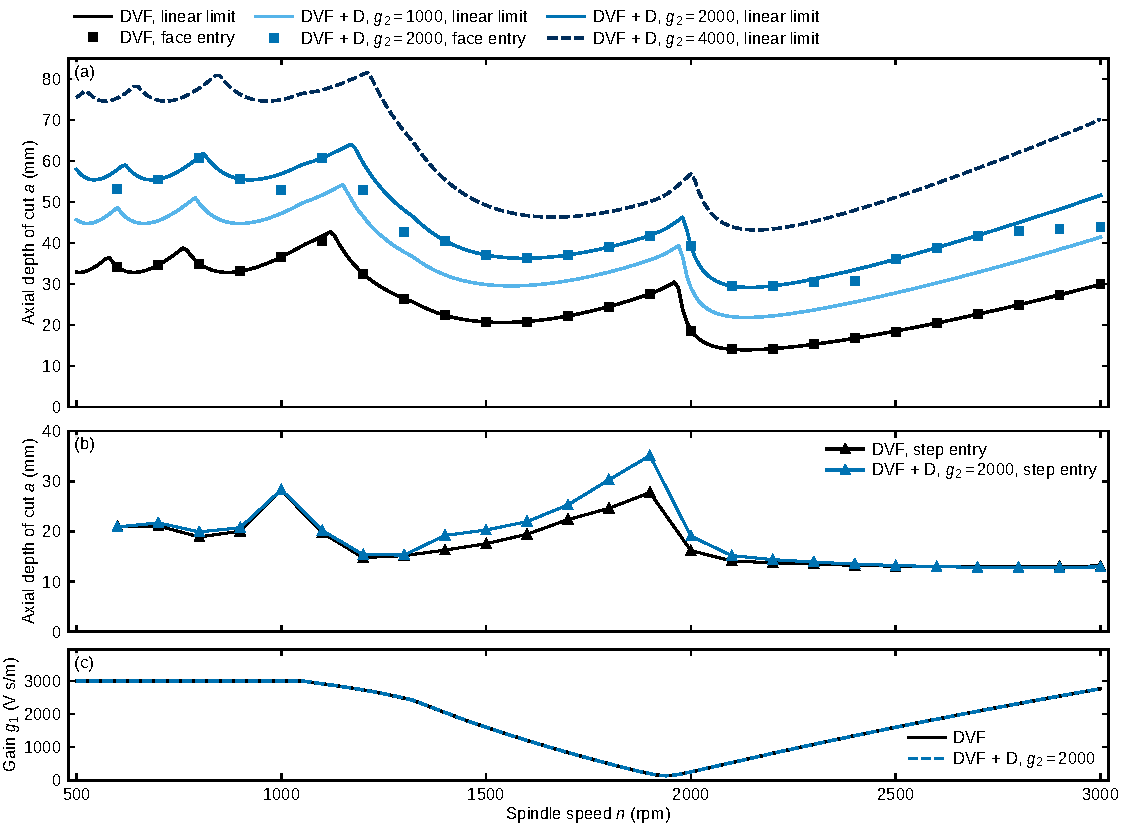
\includegraphics[width=0.86\textwidth]{figures/fig08_delayed_limits.pdf}
  \caption{The delayed term under the same authority rule ($g_1\le\SI{3000}{\volt\second\per\metre}$; steady forced command within \SI{9}{\volt} up to 0.9 of the design's own $\alim$). (a)~Linear limits of DVF and of DVF\,+\,D with $g_2=1000$, 2000 and \SI{4000}{\volt\second\per\metre}; squares: simulated face-entry limits ($\lvert V\rvert\le\SI{9}{\volt}$, 25 speeds) of DVF and of DVF\,+\,D with $g_2=2000$; dash-dotted: $2D=\SI{32}{\milli\metre}$, twice the cutter diameter. (b)~Simulated step-entry limits of the same two designs: the linear margin gained by the delayed term hardly reaches the clipped step entry.}
  \label{fig:dlim}
\end{figure}

The case study thus gives a negative result that matters for design: a law that raises the linear limit by 78\,\% and spends no authority on the forced orbit raises the depth reached by an abrupt entry by 3\,\%, because the entry transient, not the damping of the chatter mode, saturates the actuator. Linear margin is not tolerance of disturbances.

\subsection{Robustness of the residual authority and of the basin}\label{supp:std-delayed-robust}

The residual authority of the nominal design was sampled under errors in the model (Table~\ref{tab:mc}). The cutting coefficients were drawn independently and uniformly within $\pm\SI{10}{\percent}$ of their nominal values (in a second case $\pm\SI{20}{\percent}$), the natural frequency within $\pm\SI{5}{\percent}$, the damping ratio within $\pm\SI{20}{\percent}$, the actuator force constant within $\pm\SI{10}{\percent}$, the eccentric runout within 0--\SI{5}{\micro\metre}, the clip level within 8.1--\SI{9}{\volt} and the loop delay within 0--\SI{300}{\micro\second}; for 4000 samples per case the linear limit and the forced command, the worst over eight phases of the runout, of the $g=1500$ design were computed in closed form at depths fixed as fractions of the nominal $\alim$. At the design depth $0.9\,\alim$ the sampled cut is linearly unstable in 8--\SI{20}{\percent} of the samples, and its forced orbit reaches the clip in up to \SI{9}{\percent}; at $0.98\,\alim$ the two together take 32--\SI{79}{\percent}. Even at half the limit, the forced orbit reaches the clip in 69 and \SI{50}{\percent} of the samples at 2500 and \SI{2870}{\rpm}, where the nominal residual authority is only 1.5 and \SI{3.2}{\volt} at that depth. There the runout dominates (Spearman rank correlation with $u_0$ of $-0.62$ and $-0.83$), whereas near the limit the cutting coefficient, the natural frequency and the actuator constant dominate through the linear limit itself. Widening the range of the cutting coefficients to $\pm\SI{20}{\percent}$ raises the probability of linear instability at $0.9\,\alim$ to 15--\SI{22}{\percent}. In the simulator, with the sampled runout, clip and loop delay, the worst-phase critical kick at $0.9$ of the nominal $\alim$ was found for the first 25 samples at each speed (Section~\ref{supp:mc}). In one or two of them per speed the cut did not settle, being linearly unstable at the sampled parameters or, at \SI{2870}{\rpm}, its forced command exceeding the clip by several volts. In 92 of the other 93 samples the critical kick was 0.39--2.04 times its nominal value (medians 0.81--1.16 over the speeds) and below half of it in three, and in one no kick up to \SI{3}{\metre\per\second} ended in chatter. It followed the margin to the sampled linear limit (rank correlation 0.64--0.90) more closely than the residual authority (0.21--0.43), except at \SI{2870}{\rpm} (0.67 against 0.74), where the runout dominates the latter. Such samples show how the basin moves with the errors but bound nothing: with one or two unsettled samples in 25, the 95\,\% upper confidence bound on that probability is 18--\SI{23}{\percent}.
% src: verification/paper/mc_closed_form.json (levels.pm10/pm20.ranges; n_per_case 4000; speeds.*.fracs.*.p_unstable, p_saturated, u0_stable_median_V, dominant_u0_all, spearman_u0_all: 2500 rpm 0.5 runout -0.62, 2870 rpm 0.5 runout -0.83; nominal.u0_9V); mc_closed_form.py, mc_common.py (caches restored; nominal reproduces stored a_lim and bmax: checks.nominal)
% src (simulated): verification/paper/mc_kick.py/.json (protocol: first 25 samples of the pm10 draw, seed 20261124, 0.9 nominal a_lim, g 1500, phases 0/4/8/12 of 16, face entry, full memory, judged once per revolution); verification/paper/mc_kick_stats.py/.json (speeds.*: unsettled 2/2/1/2, unsettled_reasons linearly unstable at 1090/1420/2500, forced command at the clip at 2870; inf 1/0/0/0; finite 22/23/24/23; all.ratio_min 0.386, ratio_max 2.044, ratio_median_range 0.805-1.158; below_half_nominal 0/2/1/0; spearman_kick_vs_alim_margin 0.879/0.904/0.641/0.673; spearman_kick_vs_u0_worst_psi 0.209/0.416/0.432/0.735; cp95_upper_unsettled 0.231/0.231/0.176/0.231)

\begin{table}[!tbp]
  \centering
  \caption{Monte Carlo of the residual authority $u_0=V_{\mathrm{clip}}-\bmax$ of the $g=\SI{1500}{\volt\second\per\metre}$ design (closed-form zero-order model; forced command the worst over eight runout phases; 4000 samples per case; depth fixed at a fraction of the nominal $\alim$; parameter ranges in the text). $\pm\SI{10}{\percent}$, $\pm\SI{20}{\percent}$: range of the cutting coefficients. $u_0$ in volts; median over the linearly stable samples. Unstable: linearly unstable samples; clip: stable samples whose forced orbit reaches the clip ($u_0\le0$); both in per cent of the samples. These are frequencies over an assumed distribution, not a guarantee.}
  \label{tab:mc}
  \small
  \begin{tabular}{@{}rcccccrr@{}}
    \toprule
    Speed & $a/\alim$ & Nominal & \multicolumn{3}{c}{$\pm\SI{10}{\percent}$} & \multicolumn{2}{c}{$\pm\SI{20}{\percent}$}\\
    \cmidrule(lr){4-6}\cmidrule(l){7-8}
    (rpm) & & $u_0$ & median $u_0$ & unstable & clip & unstable & clip\\
    \midrule
    1090 & 0.5 & 4.72 & 3.69 & 0 & 0 & 0 & 0\\
     & 0.7 & 4.65 & 3.71 & $<1$ & 0 & 1 & 0\\
     & 0.9 & 4.69 & 3.96 & 20 & 0 & 20 & 0\\
     & 0.98 & 4.01 & 3.20 & 32 & 0 & 31 & 0\\
    \addlinespace
    1420 & 0.5 & 2.68 & 1.80 & 0 & $<1$ & 0 & 2\\
     & 0.7 & 8.72 & 7.79 & 0 & 0 & 0 & 0\\
     & 0.9 & 2.91 & 1.98 & 12 & $<1$ & 22 & 1\\
     & 0.98 & 1.79 & 1.21 & 48 & 2 & 49 & 2\\
    \addlinespace
    2500 & 0.5 & 1.49 & -0.65 & 0 & 69 & 0 & 65\\
     & 0.7 & 7.76 & 6.14 & 0 & 0 & $<1$ & 0\\
     & 0.9 & 2.79 & 1.58 & 11 & 4 & 15 & 8\\
     & 0.98 & 1.13 & -0.63 & 31 & 48 & 33 & 39\\
    \addlinespace
    2870 & 0.5 & 3.24 & 0.01 & 0 & 50 & 0 & 49\\
     & 0.7 & 5.99 & 2.29 & 0 & 19 & 0 & 19\\
     & 0.9 & 6.74 & 4.12 & 8 & 9 & 15 & 7\\
     & 0.98 & 5.04 & 3.30 & 34 & 3 & 39 & 2\\
    \bottomrule
  \end{tabular}
\end{table}
% src: verification/paper/mc_closed_form.json (nominal.<rpm>.u0_9V; levels.pm10/pm20.speeds.<rpm>.fracs.<frac>: u0_stable_median_V, p_unstable, p_saturated)

The clip level itself is a design choice (Section~\ref{supp:std-model-act}). Lowering it from 9 to \SI{8.1}{\volt}, which kept the peak actuator force at \SI{26.6}{\newton} in the deepest stable step entry at \SI{2500}{\rpm}, reduces the residual authority at $0.9\,\alim$ to 0.68--0.87 of its value and the worst-phase critical kick there to 0.76--0.88 of its value at the four speeds, close to the ratios of 0.78--0.89 that the describing function of Eq.~\eqref{M-eq:dfbasin} predicts; at \SI{2500}{\rpm} the forced command exceeds \SI{8.1}{\volt} already at 0.27--$0.46\,\alim$, by up to \SI{0.47}{\volt}, and again near $\alim$, so that with this clip the forced orbit itself is clipped there and the basin closes before the limit. A force limit enforced by lowering the clip is thus paid for in tolerated disturbance.
% src: verification/paper/protocol_clip_level.json (summary: ratio_of_minima 0.850/0.763/0.763/0.878 at 1090/1420/2500/2870 rpm, 0.9 a_lim, phases 0, 4, 8, 12; df_ratio_prediction 0.845/0.801/0.778/0.892; free_voltage_ratio_at_0p9alim 0.808/0.690/0.677/0.866; free_voltage_ratio_at_alim at 2500 rpm -0.038); verification/paper/support_runs.json (26.6 N at 8.1 V, deepest stable step entry at 2500 rpm, g = 1500); verification/paper/clip81_forced_command.py/.json (2500 rpm: intervals_above_clip_frac 0.27-0.46 and 0.9975-1, max_V 8.570 at 0.35 a_lim, V_at_a_lim 8.13; none at 1090, 1420, 2870 rpm)


\subsection{Monte Carlo of the residual authority}\label{supp:mc}

\paragraph{Closed form} The cutting coefficients $K_{tc}$ and $K_{rc}$ were drawn independently and uniformly within $\pm\SI{10}{\percent}$ (and, with the same uniform draws, within $\pm\SI{20}{\percent}$) of their nominal values, the natural frequency within $\pm\SI{5}{\percent}$ with the stiffness fixed, the damping ratio within $\pm\SI{20}{\percent}$, the actuator constant $K_a$ within $\pm\SI{10}{\percent}$, the eccentric runout within 0--\SI{5}{\micro\metre}, the clip within 8.1--\SI{9}{\volt} and the loop delay within 0--\SI{300}{\micro\second}, 4000 samples per case. For each sample the linear limit of the delayed DVF loop of the $g=1500$ design was computed in the zero-order model, and the forced command at the fixed depth as the worst over eight runout phases; with 32 phases the command rises by at most \SI{15}{\milli\volt}. The nominal sample reproduces the stored limits, free voltages and runout tolerances. With the runout set to zero, the probability that the forced orbit reaches the clip at half the limit falls from 69 to \SI{33}{\percent} at \SI{2500}{\rpm} and from 50 to \SI{0.03}{\percent} at \SI{2870}{\rpm}.
% src: verification/paper/mc_closed_form.py, mc_common.py (ranges, seed, caches restored), mc_closed_form.json (levels.pm10.speeds.2500.fracs.0.5.no_runout.p_saturated 0.328, 2870 0.00025; checks.nominal reproduces the stored a_lim, free voltage and runout tolerance; n_psi_8_vs_32 max_underestimate_V 0.0152)

\paragraph{Simulated critical kick} For the first 25 samples of the $\pm\SI{10}{\percent}$ draw, at the four speeds and at 0.9 of the nominal $\alim$ ($g=\SI{1500}{\volt\second\per\metre}$), the cut was simulated with the sampled parameters, its own runout amplitude and phase, clip and loop delay, the full surface memory and a face entry, and kicked at revolution 100 at four phases a quarter of a tooth period apart, with the kick search of Section~\ref{M-sec:bistab-prot}; a phase was abandoned as soon as its critical kick was proven larger than the smallest so far, which leaves the minimum unchanged. With runout the settled orbit is periodic in the spindle revolution, which the tooth-period classifier would call chatter, so the runs were judged once per revolution with the same thresholds; with the tooth-period classifier the nominal runs reproduce the stored critical kicks exactly. A sampled delay shorter than one time step of the simulator (41--\SI{107}{\micro\second}) was simulated as zero or one step, and the closed-form values of the sample were recomputed with the delay simulated. Table~\ref{tab:mc-kick} gives the results. Seven samples did not settle: five that are linearly unstable at the sampled parameters, and the two at \SI{2870}{\rpm} whose forced command exceeds the sampled clip by 2.9 and \SI{14.5}{\volt}. Two samples that the closed form calls marginally unstable (by 0.5 and \SI{0.3}{\percent} in depth), and two at \SI{2500}{\rpm} whose forced command exceeds the sampled clip by up to \SI{0.35}{\volt}, settled nonetheless and have finite critical kicks.

\begin{table}[!tbp]
\centering
\caption{Simulated worst-phase critical kick (four phases) under the sampled errors of Table~\ref{tab:mc}, 25 samples per speed, $a=0.9\,\alim$ (nominal), $g=\SI{1500}{\volt\second\per\metre}$. Not settled: chatter before the kick. Ratio: critical kick over its nominal value, over the samples with a finite critical kick. $\rho_s$: Spearman rank correlation of the critical kick with the margin $\alim-a$ of the sample and with its residual authority $u_0$ (worst runout phase).}
\label{tab:mc-kick}
\small
\setlength{\tabcolsep}{4pt}
\begin{tabular}{@{}rccccccc@{}}
\toprule
Speed & Nominal & Not & No chatter & Ratio, median & Below & \multicolumn{2}{c}{$\rho_s$ with}\\
\cmidrule(l){7-8}
(rpm) & (\si{\milli\metre\per\second}) & settled & to \SI{3}{\metre\per\second} & (range) & half & $\alim-a$ & $u_0$\\
\midrule
1090 & 15.1 & 2 & 1 & 1.16 (0.62--2.04) & 0 & 0.88 & 0.21\\
1420 & 12.9 & 2 & 0 & 0.81 (0.39--1.83) & 2 & 0.90 & 0.42\\
2500 & 7.3  & 1 & 0 & 0.92 (0.48--1.79) & 1 & 0.64 & 0.43\\
2870 & 11.6 & 2 & 0 & 0.81 (0.51--1.19) & 0 & 0.67 & 0.74\\
\bottomrule
\end{tabular}
\end{table}
% src: verification/paper/mc_kick.py/.json (protocol, nominal.*.worst4_rev_mmps 15.058/12.939/7.288/11.611, worst4_tooth equal; samples.*.tau_sim; cf); verification/paper/mc_kick_stats.py/.json (speeds.*: unsettled 2/2/1/2, inf 1/0/0/0, ratio_median 1.158/0.814/0.917/0.805, ratio_min/max 0.621-2.044, 0.386-1.834, 0.484-1.795, 0.505-1.189, below_half_nominal 0/2/1/0, spearman_kick_vs_alim_margin 0.879/0.904/0.641/0.673, spearman_kick_vs_u0_worst_psi 0.209/0.416/0.432/0.735; cf_unstable_but_settled: sample 11 at 1090 rpm, a_lim 18.80 against 18.89 mm, sample 14 at 1420 rpm, 15.95 against 16.00 mm; mc_kick.json samples: 2870 rpm samples 0 and 19 unsettled with cf.u0_worst_psi_V -2.91 and -14.46; 2500 rpm samples 13 and 17 settled with u0_worst_psi_V -0.35, pre_kick_clipped true)

\subsection{The law, its properties and prior work}\label{supp:delayed-prior}

In the notation of Section~\ref{M-sec:delayed-law}, $K(s)=g_1+g_2E(s)$ and $E(s)=1-e^{-sT}$; the law with $g_2=0$ and $k_d\neq0$ is denoted DVF\,+\,P.

\emph{(ii)~DVF\,+\,D is passive only without loop delay.} For $g_1,g_2\ge0$, $\operatorname{Re}K(s)\ge g_1$ in $\operatorname{Re}s\ge0$, so $K$ is positive real and, with an ideal collocated actuator and no loop delay, the velocity loop is passive like DVF \citep{elliott2001feedback}; $\lvert K(i\omega)\rvert$ lies between $g_1$ at the harmonics and $g_1+2g_2$ halfway between them. With a loop delay $\tau$ the controller becomes $e^{-s\tau}K(s)$, and the phase of $E(i\omega)$, which falls from $+\ang{90}$ to $-\ang{90}$ between consecutive harmonics, adds to the lag of the delay in the upper half of each interval (Section~\ref{M-sec:delayed-robust}).

\emph{(iii)~$k_d$ must be negative.} As $\overline{aH}<0$ [Eq.~\eqref{M-eq:aHmean}] and $G_a\approx K_a$ at the chatter frequency, $k_d=\SI{-e5}{\volt\per\metre}$ adds about \SI{3e5}{\newton\per\metre} to the negative coefficient of $x-x(t-T)$, as much as $\lvert\overline{aH}\rvert$ at $a=\SI{1}{\milli\metre}$, and so offsets about \SI{1}{\milli\metre} of depth.
% src: README §13.2; src/c4_comb.py (docstring, model), src/c4_robust.py (controller); tests/test_c4_comb.py (test_comb_terms_vanish_on_the_settled_cut; test_negative_kd_opposes_regeneration: +0.98 mm for kd = -1e5 V/m at 2500 rpm, g1 = 1500); N_t K_tc |alpha_yy|/(4 pi) x 1 mm = 3.0008e5 N/m from src/params.py; |G_a|/K_a = 1.004 at 129.3 Hz (Section 2.1)

The law is published. Its non-invasiveness on the periodic orbit is that of Pyragas-type delayed feedback \citep{pyragas1992continuous}, which \citet{vandewouw2015ifac} and \citet{vandijk2015ijrnc} applied to high-speed milling, the latter with fixed-structure delayed output feedback that vanishes on the periodic solution and with the actuator forces as a design criterion. \citet{li2022ijamt} fed back $x(t)-x(t-T)$ through a PD law to lower the actuator voltage, delayed feedback has countered the regenerative effect in turning \citep{mancisidor2019mechatronics} and milling \citep{du2022time}, and \citet{du2024ijms} combined it with robust control and reported control voltages 11--\SI{25}{\percent} below those of robust control alone, the same authority argument. What is added here is the analysis under a hard \SI{9}{\volt} clip: the authority budget left by the forced orbit, certified inner estimates of the basin with the delayed terms in the sector argument, their check in the simulator, and the robustness limits of the idealised model.
% src: README §13.2 (prior work; 11-25 % for Du et al. 2024); paper/notes/novelty.md §1.6 (descriptions from abstracts; the full text of vandewouw2015ifac was not checked)

\subsection{Models, certificate and simulator}\label{supp:delayed-model}

\paragraph{Certificate}
The averaged collocation model~\eqref{M-eq:coll} keeps its form, with the DVF row $k^\top=-g\,e_2^\top$ replaced by
\begin{equation*}
  \begin{gathered}
    k^\top=-(g_1+g_2)\,e_2^\top+g_2\,d_N^\top-k_d\,\bigl(e_1-e_{4+N}\bigr)^\top,\\
    d_N^\top\xi=\frac2T\Bigl[(D_N)_{N0}\,\tilde x+\sum_{l=1}^{N}(D_N)_{Nl}\,\tilde x(t+\vartheta_l)\Bigr],
  \end{gathered}
\end{equation*}
where $e_{4+N}^\top\xi=\tilde x(t-T)$ and $d_N^\top\xi$, the derivative of the Chebyshev interpolant of the history at $\vartheta=-T$ (Section~\ref{app:lmi}), stands for $\dot{\tilde x}(t-T)$. As $b(t)$ depends on $g_1$ only, $\bar b$, the sector condition~\eqref{M-eq:sector}, the LMIs \eqref{M-eq:lmi-dec}--\eqref{M-eq:lmi-size} and the check of Section~\ref{M-sec:cert-check} apply unchanged. A velocity kick $\Delta v$, however, leaves a kink in the history that the interpolant smooths, and the delayed command of the model then departs from that of the delay equation by about half of $g_2\Delta v$ in each of the first two tooth periods (DVF: less than \SI{1}{\percent} of $g\Delta v$); the certificate therefore rests more on the simulator check (Section~\ref{supp:delayed-valid}) than in Section~\ref{M-sec:certificates}.
% src: src/c4_comb.py (model, certify_kick; docstring: 0.45-0.5 and 0.5-0.65 g2 per m/s of kick); tests/test_c4_comb.py (test_comb_model_without_comb_is_the_c2_model, test_comb_row_vanishes_on_a_tooth_periodic_state, test_comb_limit_converges_in_the_nodes: limit moves < 1e-4 with 1.6x and 2.4x the nodes at 2500 rpm); README §13.3

\paragraph{Simulator and closed form}
The simulator of Section~\ref{app:simulator} was extended by $g_2$, $k_d$, a comb delay $T_c$ in place of $T$, eccentric runout of the teeth and a loop delay $\tau$. The robustness study uses the averaged model in the frequency domain, with the characteristic function
\begin{equation}\label{eq:comb-char}
  \begin{aligned}
    \Delta(s)&=1-G(s)\Bigl[\overline{aH}\,E(s)-G_a(s)\,e^{-s\tau}\bigl(s\,[g_1+g_2E_c(s)]+k_d\,E_c(s)\bigr)\Bigr],\\
    E_c(s)&=1-e^{-sT_c},
  \end{aligned}
\end{equation}
where $G$ may include an assumed second mode; with $\tau=0$, $T_c=T$ and one mode, $\Delta=0$ is the characteristic equation of the averaged delay equation. Its limits agree with those of the collocation model and of the simulator (Supplementary Material).
% src: README §13.3; src/tdsim.c (COMB build); src/c4_robust.py (delta, unstable_zeros); tests/test_c4_comb.py (test_closed_form_limit_is_the_collocated_limit, 4 cases, rel 2e-4); results/c4_robust.npz and c4_summary.json (robust.td_limit_ratio 1.0025-1.0148, 7 cases)

\subsection{A fair baseline and the linear limit}\label{supp:delayed-limit}

The bound $g\le\SI{1500}{\volt\second\per\metre}$ of Sections~\ref{M-sec:feasibility}--\ref{M-sec:certificates} is a choice of this study, not a property of the actuator, and a comparison at that bound inflates the benefit: added to those gains, $g_2=\SI{2000}{\volt\second\per\metre}$ doubles the linear limit (median ratio 2.0). Both families were therefore designed by the rule of Eq.~\eqref{M-eq:feas}: $g_1$ is the largest gain up to \SI{3000}{\volt\second\per\metre} whose steady forced command stays within \SI{9}{\volt} up to 0.9 times the design's own linear limit. For DVF this is the map with $g_{\max}=3000$ of Section~\ref{M-sec:feas-res}, limited by authority at 195 of the 251 speeds and by the bound at the other 56. Adding $g_2$ or $k_d$ hardly changes $g_1$ (Supplementary Material), so in effect the same gain is compared with and without the delayed term.
% src: results/c4_limits.npz (a_lim at the C1/C2 gain + g2 = 2000: median ratio 2.005; feas_g1: DVF below 3000 at 195 speeds, 1060-3000 rpm; max |g1 - g1_DVF| = 9.7 V s/m, 0.35 %); results/c4_summary.json (limits); src/c4_comb.py (a_lim_ctrl, feasible_g1); tests/test_c4_comb.py (test_feasible_dvf_gain_is_the_feasibility_optimum); README §13.4

With $g_2=2000$ the limit rises by a median factor of 1.78 (1.44--2.10; Table~\ref{tab:dlim}, Fig.~\ref{fig:dlim}a). The rise persists where DVF sits on the bound: with the bound lifted to \SI{20000}{\volt\second\per\metre} for both families at those 56 speeds, DVF\,+\,D still reaches a median 1.47 times the DVF limit, so the D term adds linear margin rather than only redistributing authority. Much of the gain, however, lies at large depths: with $g_2=2000$ the limit exceeds \SI{32}{\milli\metre}, twice the cutter diameter, at 222 of the 251 speeds, against 71 for DVF, and with the usable depth capped at \SI{32}{\milli\metre} the median gain falls from 1.78 to 1.31; the cutting tests of \citet{ozsoy2026robust} went up to \SI{10}{\milli\metre}. The P term shifts the limit by a nearly constant amount, about \SI{1}{\milli\metre} per \SI{-e5}{\volt\per\metre} of $k_d$, as (iii) predicts (Supplementary Material).
% src: results/c4_summary.json (limits.feasible; limits.uncapped: 56 speeds, d2000/DVF 1.31-1.68, median 1.47); results/c4_limits.npz (feas_a_lim differences, recomputed: p3e5 - dvf 2.89-3.02 mm, p1e6 - dvf 9.66-9.93 mm); README §13.4, §13.5
% src (depth qualifier): verification/paper/revision_runs.json (stored.depth_2D: d2000_above_32mm 222, dvf_above_32mm 71 of 251 speeds; median_ratio 1.781, median_ratio_capped_32mm 1.309), recomputed from results/c4_limits.npz (feas_a_lim, feas_names); cutter diameter 16 mm (Table 1); verification/targets/experimental_points.csv (tested depths up to 10 mm)

\begin{table}[!htbp]
  \centering
  \caption{Linear stability limit over 251 speeds (\SIrange{500}{3000}{\rpm}) under the same authority rule [Eq.~\eqref{M-eq:feas} with the design's own $\alim$, $g_1\le\SI{3000}{\volt\second\per\metre}$]; $g_2$ in \si{\volt\second\per\metre}. Ratio to the DVF limit at the same speed: median (range) over all speeds; last column: median over the 195 speeds where the DVF gain is limited by authority / over the 56 where it sits on the bound. The DVF\,+\,P designs are given in the Supplementary Material.}
  \label{tab:dlim}
  \small
  \begin{tabular}{@{}lccc@{}}
    \toprule
    Design & $\alim$ (\si{\milli\metre}) & Ratio to DVF & Median ratio\\
     & & median (range) & authority / bound\\
    \midrule
    DVF & 14.0--42.8 & 1 & --\\
    DVF\,+\,D, $g_2=1000$ & 21.9--54.3 & 1.43 (1.23--1.57) & 1.43 / 1.34\\
    DVF\,+\,D, $g_2=2000$ & 29.2--64.1 & 1.78 (1.44--2.10) & 1.81 / 1.64\\
    DVF\,+\,D, $g_2=4000$ & 43.2--81.6 & 2.40 (1.75--3.15) & 2.50 / 2.20\\
    \bottomrule
  \end{tabular}
\end{table}
% src: results/c4_summary.json (limits.feasible: a_lim_mm, ratio_to_dvf, ratio_authority_limited, ratio_gain_bounded); results/c4_limits.npz; README §13.5



\subsection{Entries in the simulator}\label{supp:delayed-entry}

Step and face entries (Section~\ref{M-sec:bistab-prot}) were simulated with the \SI{9}{\volt} clip at 25 speeds (\SIrange{600}{3000}{\rpm}) for DVF and for DVF\,+\,D with $g_2=2000$ (Fig.~\ref{fig:dlim}a,b). With D the face-entry limit is 1.45--2.12 times higher (median 1.72) and reaches the new linear limit at 16 of the 25 speeds (0.85--$0.98\alim$ at the others). The step-entry limit changes little: the ratio is 0.98--1.27 (median 1.03). From \SI{2100}{\rpm} upwards D changes it by at most \SI{1.1}{\milli\metre}, as this limit is set by saturation during the entry, not by damping; only at \SIrange{1400}{2000}{\rpm}, where the step entry approaches the linear limit, does D raise it markedly (1.13--1.27 times).
% src: results/c4_entry.npz (designs feas_dvf, feas_d2000: a_entry, a_lim, g1; per-speed ratios: face 1.45-2.12, median 1.72; face entry with D at a_lim at 16 speeds, 0.85-0.98 a_lim at nine; step 0.98-1.27, median 1.03; 1.13-1.27 at 1400-2000 rpm, 1.008 at 1300 rpm, recomputed; from 2100 rpm +1.08 mm at most, -0.21 mm at most at 2700-3000 rpm); README §13.6

The band between the step-entry and the linear limit, in which the outcome depends on the entry, therefore widens: the median ratio of the two limits falls from 0.70 for DVF to 0.39 with D, and the median width of the band grows from 7.6 to \SI{26}{\milli\metre}. Most of the depth gained needs a gentle entry.
% src: results/c4_entry.npz (step/a_lim medians 0.704 and 0.390; a_lim - step medians 7.56 and 25.88 mm); README §13.6

\subsection{Certified gain map}\label{supp:delayed-map}

The certified kick $\beta$ [Eq.~\eqref{M-eq:lmi-size} with $e=e_2$] was computed at the four speeds of Section~\ref{M-sec:bistab-basin} and 17 depths (2--\SI{34}{\milli\metre}) for 20 delayed pairs, $g_1\in\{500,1000,1500,2000,3000\}$ and $g_2\in\{500,1000,2000,4000\}$\,\si{\volt\second\per\metre}, and for DVF at 26 gains (500--\SI{3000}{\volt\second\per\metre} in steps of 100), so that DVF has no fewer candidates. Table~\ref{tab:dgap} gives the depth up to which every grid depth is certified with a kick of at least $\beta_{\mathrm{th}}$. At $\beta_{\mathrm{th}}=\SI{1}{\milli\metre\per\second}$ the delayed term covers the whole grid at all four speeds, against 16--\SI{34}{\milli\metre} for DVF, and the advantage narrows as $\beta_{\mathrm{th}}$ grows. These thresholds are small: as equivalent displacements $\beta_{\mathrm{th}}/\omega_n$, 1, 2 and \SI{4}{\milli\metre\per\second} are 1.2, 2.5 and \SI{4.9}{\micro\metre}, and a kick of \SI{1}{\milli\metre\per\second} carries only 0.5--\SI{1.3}{\percent} of the cutting impulse of one tooth period [Eq.~\eqref{M-eq:impulse}] at \SI{16}{\milli\metre}, whereas kicks of 2.4--\SI{10.8}{\percent} tip the clipped DVF cut into chatter near its limit (Section~\ref{M-sec:bistab-basin}).
% src: src/c4_comb.py (GM_RPM, GM_DEPTH, GM_G1, GM_G2, GM_G1_DVF; run_gainmap); results/c4_gainmap.npz; results/c4_summary.json (gainmap.by_rpm.certified_without_gap_mm); results/c3_summary.json (errata.c4_gainmap: size_factor 0.593-1, table unchanged); impulse shares recomputed from Eq. (impulse) with src/params.py: 0.48-1.25 % at 16 mm; beta_th / omega_n with omega_n = 2 pi x 129.3 rad/s (src/params.py FN): 1.231, 2.462, 4.924 um; README §13.7, §14.9

The certificate picks the smallest gain with enough linear margin: with D it keeps $g_1$ at 500--1000 at most depths and raises $g_2$ to 2000--4000 where the DVF certificate is small or absent (Fig.~\ref{fig:dbasin}). Where both families are certified, the best delayed certificate exceeds the best DVF one by a median factor of only 1.05--1.08 per speed.
% src: results/c4_gainmap.npz (maximising designs per speed and depth: delayed optimum g1 = 500-1000 except at 24-26 mm and at 2870 rpm, 12 mm; g2 >= 2000 only where the best DVF certificate is 0-3.5 mm/s, recomputed); results/c4_summary.json (gainmap.by_rpm.comb_over_dvf medians 1.08, 1.05, 1.07, 1.06); README §13.7

\begin{table}[!htbp]
  \centering
  \caption{Certified depth without a gap (\si{\milli\metre}): the largest depth of the grid (2--\SI{34}{\milli\metre}, step \SI{2}{\milli\metre}) up to which every grid depth is certified with a kick of at least $\beta_{\mathrm{th}}$ by the best candidate design ($\lvert V\rvert\le\SI{9}{\volt}$; averaged collocation model, in which the delayed velocity of DVF\,+\,D is the derivative of the history interpolant, Section~\ref{supp:delayed-model}; certificates rescaled to the rigorous bound $\bar b$). $\ge34$: the whole grid.}
  \label{tab:dgap}
  \small
  \begin{tabular}{@{}llcccc@{}}
    \toprule
    $\beta_{\mathrm{th}}$ (\si{\milli\metre\per\second}) & Candidates & \SI{1090}{\rpm} & \SI{1420}{\rpm} & \SI{2500}{\rpm} & \SI{2870}{\rpm}\\
    \midrule
    1 & DVF, 26 gains & $\ge34$ & 18 & 16 & 28\\
      & DVF\,+\,D, 20 pairs & $\ge34$ & $\ge34$ & $\ge34$ & $\ge34$\\
      & DVF\,+\,D, $g_2\le2000$ & $\ge34$ & 30 & 28 & $\ge34$\\
    2 & DVF, 26 gains & 32 & 16 & 16 & 16\\
      & DVF\,+\,D, 20 pairs & $\ge34$ & 30 & 28 & $\ge34$\\
    4 & DVF, 26 gains & 26 & 16 & 14 & 14\\
      & DVF\,+\,D, 20 pairs & 28 & 26 & 16 & 18\\
    \bottomrule
  \end{tabular}
\end{table}
% src: results/c4_summary.json (gainmap.by_rpm.certified_without_gap_mm: dvf_*, comb_*, comb_g2le2000_1); results/c3_summary.json (errata.c4_gainmap.certified_without_gap_mm: unchanged by the correction); README §13.7 (table), §14.9

\subsection{Validation of the delayed designs in the simulator}\label{supp:delayed-valid2}

At the four speeds and 6--\SI{34}{\milli\metre}, 100 design points were simulated: the DVF designs with the largest certified kick over 26 and over five gains, the delayed design with the largest certified kick (the \emph{map design}) and the \emph{same-$g_1$ design}, which adds to the $g_1$ of the 26-gain DVF optimum the $g_2$ that maximises its certificate. The same-$g_1$ design has the forced orbit and the authority budget of that DVF, so any change of its basin is due to the delayed term alone. At each point the critical kick $\Delta v^*$ (worst of 16 phases), the certified kick and the critical kick of the collocation model were computed (Supplementary Material).
% src: src/c4_comb.py (VAL_DEPTH, VAL2_DEEP, best_gains, _same_g1, run_validate, run_validate2); results/c4_validate.npz (22 dvf, 24 comb), results/c4_validate2.npz (21 dvf_fine, 25 same_g1, 8 comb); README §13.8

No unkicked cut chattered. The certified kick lies below $\Delta v^*$ at all 89 points where a kick of up to \SI{3}{\metre\per\second} ended in chatter, by factors of 1.6--7.3 (median 2.3), and below the critical kick of the collocation model at all 97 points where that kick is finite. Despite the error in its delayed velocity, the collocation model reproduces $\Delta v^*$ no worse than for DVF: its critical kick is 0.80--1.01 (median 0.98) times $\Delta v^*$ for the map designs and 0.79--1.00 (median 0.96) for the same-$g_1$ designs, against 0.66--1.02 for DVF.
% src: results/c4_validate.npz, results/c4_validate2.npz (unsettled 0; td_min infinite at 11 points; model_kick infinite at 3); results/c4_summary.json (validate2: all_cert_below_td 89/89, all_cert_below_model 97/97); results/c3_summary.json (errata.c4_validate: corrected 1.60-7.32, median 2.29); README §13.8, §14.9
% src (model to simulated critical kick): results/c4_validate.npz and c4_validate2.npz recomputed: comb 29 points 0.80-1.01 (median 0.98), same_g1 22 points 0.79-1.00 (median 0.96), dvf and dvf_fine 38 points 0.66-1.02

The basins were compared at the 22 depth--speed pairs where both families have a finite $\Delta v^*$ (Fig.~\ref{fig:dbasin}). At the same forced command, the same-$g_1$ design raises $\Delta v^*$ by a median factor of 1.14 over all 22 pairs (larger at 19), by 1.45 over the 13 pairs at \SI{18}{\milli\metre} and deeper, and by 2.00 (1.79--2.59) over the six pairs, all at 18--\SI{34}{\milli\metre}, where the DVF certificate is at most \SI{2.1}{\milli\metre\per\second}; this threshold is descriptive and has no physical meaning. Below \SI{18}{\milli\metre} the basin hardly widens (0.96--1.16). The delayed term thus widens the basin through its linear margin, not by freeing authority. The certificate chose $g_2=500$, the smallest of the grid, for every same-$g_1$ design, and no other $g_2$ was simulated.
% src: results/c4_summary.json (validate2: same_g1_over_dvf 0.96-2.59, median 1.14, 19/22; same_g1_deep: 13 pairs, 1.06-2.59, median 1.45; same_g1_near_dvf_limit: DVF certified kick <= 2.1 mm/s, 6 pairs: 1420 rpm at 18 and 22 mm, 2500 rpm at 22 mm, 2870 rpm at 18 and 22 mm, 1090 rpm at 34 mm; 1.79-2.59, median 2.00; below 18 mm 0.96-1.16, recomputed from pairs_mmps); results/c4_validate2.npz (same_g1: g2 = 500 at all 25 points); README §13.8

The map design, which also frees authority, is ahead of the 26-gain DVF at 18 of the 22 pairs (median ratio 1.11), but against the better of the two DVF designs at only 13 (median 1.04). The gains that maximise the certificate are not those that maximise the basin: its preference for a small $g_1$ can narrow the basin at shallow depths (Supplementary Material).
% src: results/c4_summary.json (validate2: comb_over_dvf 0.82-3.02, median 1.11, 18/22; comb_over_better_dvf 0.81-3.02, median 1.04, 13/22; pairs_mmps); README §13.8

\begin{figure}[!htbp]
  \centering
  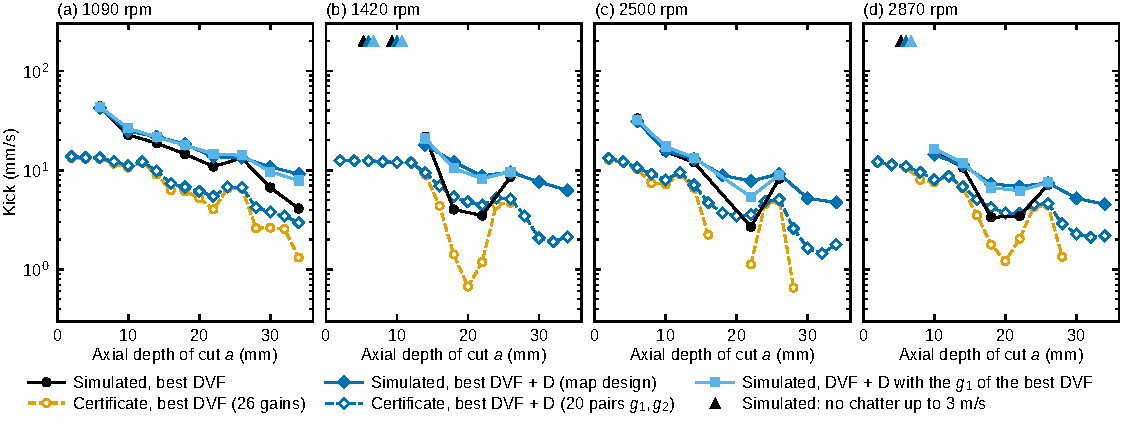
\includegraphics[width=\textwidth]{figures/fig09_delayed_basin.pdf}
  \caption{Certified and simulated kicks with the delayed term at (a)~1090, (b)~1420, (c)~2500 and (d)~\SI{2870}{\rpm} ($\lvert V\rvert\le\SI{9}{\volt}$). Open markers: certified kick of the best design at each depth over 26 DVF gains (circles) and over 20 delayed pairs $(g_1,g_2)$ (diamonds), command bound corrected; no marker: nothing certified. Filled markers: simulated critical kick $\Delta v^*$ (worst of 16 phases) of the best DVF design (26 gains), of the delayed design of the map, and of the same-$g_1$ design ($g_2=\SI{500}{\volt\second\per\metre}$ added to the $g_1$ of that DVF); triangles: no chatter for any kick up to \SI{3}{\metre\per\second} (offset horizontally for legibility).}
  \label{fig:dbasin}
\end{figure}

\subsection{Robustness of the delayed term}\label{supp:delayed-robust2}

The results above assume one mode, an instantaneous loop, a comb delay equal to $T$ and identical teeth. These assumptions were relaxed with Eq.~\eqref{eq:comb-char} at the four speeds (Table~\ref{tab:drobust}, Fig.~\ref{fig:robust}) for designs that keep \SI{10}{\percent} of the voltage free (forced command below \SI{8.1}{\volt} up to $0.9\alim$), since a design whose steady demand reaches exactly \SI{9}{\volt} at some depth, as at the authority-limited speeds of Sections~\ref{M-sec:feasibility}--\ref{M-sec:certificates}, saturates under any perturbation that raises it.
% src: src/c4_robust.py (GUARD = 0.9, designs, EPS, RUNOUT, TAU, MODE2, N_DEPTH = 40); results/c4_robust.npz (g1 1395.8-2539.5 V s/m, equal across g2 within 1.1 V s/m); README §13.9

\emph{Comb-delay error.} A speed error or a delay rounded to samples gives $T_c\neq T$, and the comb no longer vanishes on the orbit. For $g_2=2000$ and errors of $\pm\SI{2}{\percent}$ the worst forced command, 7.8--\SI{8.9}{\volt}, stays within the margin (Fig.~\ref{fig:robust}a,d), but at $+\SI{2}{\percent}$ the limit falls to 0.87--0.93 of its nominal value, into the design depths at three of the four speeds (Supplementary Material).
% src: results/c4_robust.npz, results/c4_summary.json (robust.by_rpm, tooth comb: eps_a_lim_mm, eps_worst_cmd_V); paper/figures/figure_numbers.json (fig10: eps_plus2_rel 0.87-0.93, eps_pm2_worst_cmd 7.76-8.89 V); README §13.9

\emph{Runout.} Eccentric runout makes the forced orbit spindle-periodic, so the comb acts on it, as does the regeneration. The runout at which the worst forced command reaches \SI{9}{\volt} therefore falls as $g_2$ grows, except from DVF to $g_2=1000$ at \SI{2870}{\rpm} (Table~\ref{tab:drobust}; Fig.~\ref{fig:robust}b,e); a comb with the spindle period, which vanishes on the runout orbit, is no remedy (Supplementary Material).
% src: results/c4_summary.json (robust.by_rpm: runout_tolerance_um, DVF/1000/2000/4000 in um: 1090 rpm 3.63/3.22/2.42/1.73, 1420 rpm 4.50/1.98/1.75/1.27, 2500 rpm 1.55/1.50/1.33/0.84, 2870 rpm 1.12/1.22/1.03/0.69, monotone except DVF to 1000 at 2870 rpm); src/c4_robust.py (worst_orbit_command: N_DEPTH = 40, n_psi = 8); README §13.9

\emph{Loop delay and assumed higher modes.} With the identified mode alone, DVF\,+\,D loses limit gradually with the loop delay and stays above DVF up to \SI{400}{\micro\second}. A second mode, not identified for this set-up, was assumed at 400, 600 or \SI{800}{\hertz} ($k_2=6k$, $6k$ or $40k$; $\zeta_2=\SI{1}{\percent}$). With the \SI{400}{\hertz} mode and \SI{300}{\micro\second}, $g_2=2000$ falls below DVF at all four speeds, and with the \SI{600}{\hertz} mode and \SI{200}{\micro\second} its limit collapses, while $g_2=1000$ stays above DVF (Fig.~\ref{fig:robust}c,f). The cause is the phase of the comb, not its gain: DVF with the constant gain $g_1+2g_2$ keeps a limit more than three times larger under the same delay and mode. The tolerances of Table~\ref{tab:drobust} are read off six computed delays with the criterion $\alim(\tau)\ge0.5\,\alim(0)$ and the three assumed modes, so the families differ by one step of that grid; they illustrate a trend and are not delay margins. The effect of the loop delay on the basin of the clipped loop, and the sensor noise amplified by $\lvert K\rvert$ up to $g_1+2g_2$, were not examined.
% src: results/c4_summary.json (robust.by_rpm tau_a_lim_mm: one mode, g2 = 2000 above DVF at every delay up to 400 us; mode_400Hz at 300 us 10.99-22.37 against 17.06-40.06 mm; mode_600Hz at 200 us 4.41-12.92 mm, g2 = 1000 23.74-46.84 mm against DVF 16.79-40.44 mm); src/c4_robust.py (TAU: 0, 50, 100, 200, 300, 400 us; MODE2); tests/test_c4_comb.py (test_comb_fragility_to_delay_is_its_phase_not_its_gain: limit with g1 + 2 g2 more than 3 times that of the comb); README §13.9; paper/figures/figure_numbers.json (fig10: loop_delay_largest_with_ratio_ge_05_us, second_modes_f_kratio_zeta)

\begin{table}[!htbp]
  \centering
  \caption{Robustness at 1090, 1420, 2500 and \SI{2870}{\rpm} (ranges over the speeds; closed-form zero-order model; forced command below \SI{8.1}{\volt} up to $0.9\alim$). Runout: eccentric runout at which the largest forced command over the design depths and eight runout phases reaches \SI{9}{\volt}. Loop delay: largest of the computed delays (0, 50, 100, 200, 300, \SI{400}{\micro\second}) with $\alim(\tau)\ge0.5\,\alim(0)$ at every speed and for each assumed second mode (400, 600 or \SI{800}{\hertz}).}
  \label{tab:drobust}
  \small
  \begin{tabular}{@{}lcccc@{}}
    \toprule
     & DVF & \multicolumn{3}{c}{DVF\,+\,D, $g_2$ (\si{\volt\second\per\metre})}\\
    \cmidrule(l){3-5}
     & & 1000 & 2000 & 4000\\
    \midrule
    Linear limit (\si{\milli\metre}) & 15.9--37.6 & 24.6--47.1 & 32.1--55.4 & 45.8--70.5\\
    Runout tolerated (\si{\micro\metre}) & 1.12--4.50 & 1.22--3.22 & 1.03--2.42 & 0.69--1.73\\
    Loop delay tolerated (\si{\micro\second}) & 300 & 200 & 100 & 100\\
    \bottomrule
  \end{tabular}
\end{table}
% src: results/c4_summary.json (robust.by_rpm: a_lim_mm, runout_tolerance_um, tau_a_lim_mm); paper/figures/figure_numbers.json (fig10: runout_tolerated_um, loop_delay_largest_with_ratio_ge_05_us); README §13.9 (table)

\begin{figure}[!htbp]
  \centering
  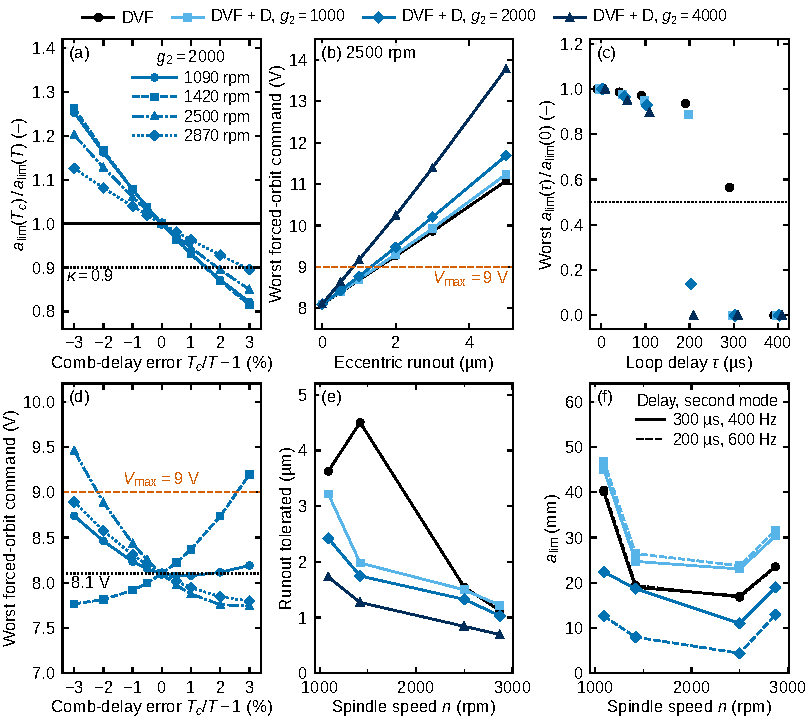
\includegraphics[width=\textwidth]{figures/fig10_robustness.pdf}
  \caption{Robustness of the delayed term (closed-form zero-order model; designs as in Table~\ref{tab:drobust}). (a)~Linear limit against the comb-delay error, relative to the exact delay ($g_2=\SI{2000}{\volt\second\per\metre}$), and (d)~worst forced-orbit command in the same cases. (b)~Worst forced-orbit command at \SI{2500}{\rpm} against the eccentric runout, and (e)~the runout at which it reaches \SI{9}{\volt}. (c)~$\alim(\tau)/\alim(0)$, worst over the four speeds and the three assumed second modes, at the computed delays only (0: loop unstable without cutting; dotted: 0.5; markers offset horizontally for legibility). (f)~$\alim$ of DVF and of DVF\,+\,D with $g_2=1000$ and 2000, with \SI{300}{\micro\second} and the \SI{400}{\hertz} mode (solid) or \SI{200}{\micro\second} and the \SI{600}{\hertz} mode (dashed); $g_2=4000$, unstable without cutting in both cases, is not shown.}
  \label{fig:robust}
\end{figure}


\subsection{Simulator build}\label{supp:delayed-sim}

A second build of the simulator of Section~\ref{app:simulator}, used only when a new option is requested, adds: $g_2$ and $k_d$, with $\dot x(t-T)$ from the derivative of the cubic Hermite interpolant of the stored history (zero before $t=0$); a comb delay $T_c=\rho T$ in place of $T$ in Eq.~\eqref{M-eq:comb-law}, for a speed error ($\rho\approx1$) or a spindle-period comb ($\rho=N_t$); an eccentric radial runout $r_j=r_0\cos(2\pi j/N_t+\theta_r)$ of tooth $j$, which adds $r_j-r_{j+k}$ (indices modulo $N_t$) to the chip cut against the pass $k$ tooth periods back, so that runout enters only the regenerated chip; and a loop delay $\tau$. The default build is bit-identical to that of Sections~\ref{M-sec:feasibility}--\ref{M-sec:certificates}.
% src: README §13.3 (identical preprocessed source and disassembly, fingerprint test); src/tdsim.c (COMB build), src/c4_robust.py (runout model); tests/test_c4_comb.py (test_comb_build_with_vanishing_gains_is_the_default, test_delayed_velocity_of_the_comb_term, test_loop_delay_uses_the_motion_one_delay_back, test_spindle_comb_vanishes_on_the_runout_orbit)

\subsection{Closed-form model and its verification}\label{supp:delayed-cf}

The zeros of $\Delta(s)$, Eq.~\eqref{eq:comb-char}, in $\operatorname{Re}s>0$ were counted by the argument principle along the imaginary axis up to \SI{5}{\kilo\hertz}, in steps of \SI{0.25}{\radian\per\second}. The limit is the first depth with such a zero, found by a scan in steps of \SI{3}{\percent} from \SI{0.3}{\milli\metre} and bisection; a design whose loop is unstable without cutting is given the limit 0. The forced orbit, spindle-periodic with runout, has the harmonics $X_k=G(ik\Omega)F_k/\Delta(ik\Omega)$, with $F_k$ from the static force of one slice over a revolution, integrated over the depth as in Eq.~\eqref{M-eq:Fm} with $mN_t$ replaced by $k$ (without runout, $F_{mN_t}=F_m$).

The closed-form limits agree with those of the collocation model within $2\times10^{-4}$ (four cases), and the simulated limits are 1.003--1.015 times the closed-form ones in seven cases that include the spindle-period comb, comb-delay errors of $\pm\SI{2}{\percent}$ and loop delays of 200--\SI{400}{\micro\second}. The settled command agrees within \SI{1.3}{\percent} in seven of eight cases with runout or delay errors, and differs by \SI{0.22}{\volt} in the eighth, where it is only about \SI{1}{\volt}. The assumed second modes were not checked in the simulator.
% src: src/c4_robust.py (delta, unstable_zeros: W_MAX = 2 pi x 5 kHz, DW = 0.25 rad/s; a_lim_cf: 0 if unstable at a = 1e-7 m, scan by 3 % from 0.3 mm, bisection; slice_force_revolution, orbit_command); tests/test_c4_comb.py (test_closed_form_limit_is_the_collocated_limit, 4 cases, rel 2e-4; test_comb_limit_matches_the_simulator, 3 cases, rel 1.5 %); results/c4_robust.npz, c4_summary.json (robust.td_limit_ratio 1.0025-1.0148, 7 cases; td_orbit_ratio 0.990-1.013 in 7 cases; 0.988 V against 0.767 V, i.e. 29 %, at 1090 rpm, 25 mm, spindle comb, 3 um runout); README §13.3, §13.10

\subsection{Proportional term}\label{supp:delayed-p}

For $g_1,g_2\ge0$, $\operatorname{Re}K(s)=g_1+g_2\bigl[1-e^{-T\operatorname{Re}s}\cos(T\operatorname{Im}s)\bigr]\ge g_1$ in $\operatorname{Re}s\ge0$, which gives property (ii) of Section~\ref{supp:delayed-prior}. The P term is not passive: the real part of $k_dE(i\omega)/(i\omega)$ is $k_d\sin(\omega T)/\omega$, which changes sign. Under the authority rule of Section~\ref{supp:delayed-limit} it shifts the linear limit by a nearly constant 2.9--\SI{3.0}{\milli\metre} ($k_d=\SI{-3e5}{\volt\per\metre}$) or 9.7--\SI{9.9}{\milli\metre} ($k_d=\SI{-e6}{\volt\per\metre}$) at every speed, about \SI{1}{\milli\metre} per \SI{-e5}{\volt\per\metre} as property (iii) of Section~\ref{supp:delayed-prior} predicts (with $g_1=1500$ at \SI{2500}{\rpm}, $k_d=\SI{-e5}{\volt\per\metre}$ raises the limit by \SI{0.98}{\milli\metre}), so that its relative gain is largest where the DVF limit is small (Table~\ref{tab:supp-dlim-p}).
% src: results/c4_limits.npz (feas_a_lim differences, recomputed: p3e5 - dvf 2.89-3.02 mm, p1e6 - dvf 9.66-9.93 mm); results/c4_summary.json (limits.feasible.p3e5, p1e6); README §13.5; tests/test_c4_comb.py (test_negative_kd_opposes_regeneration: +0.98 mm for kd = -1e5 V/m at 2500 rpm, g1 = 1500)

\begin{table}[!htbp]
  \centering
  \caption{Linear stability limit of the DVF\,+\,P designs ($g_2=0$) over 251 speeds under the authority rule of Table~\ref{tab:dlim}, which they complete; $k_d$ in \si{\volt\per\metre}.}
  \label{tab:supp-dlim-p}
  \small
  \begin{tabular}{@{}lccc@{}}
    \toprule
    Design & $\alim$ (\si{\milli\metre}) & Ratio to DVF & Median ratio\\
     & & median (range) & authority / bound\\
    \midrule
    DVF\,+\,P, $k_d=-3\times10^5$ & 16.9--45.7 & 1.12 (1.07--1.21) & 1.13 / 1.09\\
    DVF\,+\,P, $k_d=-10^6$ & 23.8--52.7 & 1.40 (1.23--1.70) & 1.45 / 1.29\\
    \bottomrule
  \end{tabular}
\end{table}
% src: results/c4_summary.json (limits.feasible.p3e5, p1e6: a_lim_mm 16.91-45.71 and 23.80-52.65, ratio_to_dvf, ratio_authority_limited, ratio_gain_bounded); README §13.5

\subsection{Further details: design rule, entries and gain map}\label{supp:delayed-details}

The design's own limit in the authority rule is the first unstable depth of the collocation model, found by an upward scan and bisection, as stability need not be monotone in the depth. The DVF gain is limited by authority at \SIrange{1060}{3000}{\rpm}. Adding $g_2$ or $k_d$ changes $g_1$ by at most \SI{9.7}{\volt\second\per\metre}, because the forced demand peaks below $0.9\alim$ of either design. With the gain bound lifted to \SI{20000}{\volt\second\per\metre} at the 56 speeds where DVF sits on it, the DVF gain rises to 3010--\SI{8760}{\volt\second\per\metre}, and DVF\,+\,D ($g_2=2000$), whose $\lvert K\rvert$ peaks at $g_1+2g_2$, reaches 1.31--1.68 times the DVF limit.
% src: src/c4_comb.py (a_lim_ctrl, feasible_g1); results/c4_limits.npz (max |g1 - g1_DVF| = 9.7 V s/m); results/c4_summary.json (limits.uncapped.dvf_g1 3008-8761 V s/m; d2000/DVF 1.31-1.68); results/c4_limits.npz (feas_g1: DVF below 3000 at 195 speeds, 1060-3000 rpm); README §13.4

In the entry simulations the depth ladder was scaled to each design's own $\alim$. The face-entry limit is 14.1--\SI{40.6}{\milli\metre} for DVF and 29.5--\SI{60.8}{\milli\metre} with D; DVF reaches at least $0.97\alim$, and with D it stays at 0.85--$0.98\alim$ at 600, 1000, 1200, 1300, 2300, 2400 and 2800--\SI{3000}{\rpm}. The step-entry limit is 12.9--\SI{28.2}{\milli\metre} for DVF and 12.7--\SI{35.1}{\milli\metre} with D; D raises it by up to 1.27 times at \SI{1900}{\rpm} and lowers it by up to \SI{0.2}{\milli\metre} at \SIrange{2700}{3000}{\rpm}. At \SIrange{600}{1300}{\rpm} the larger DVF gain of this rule (2480--\SI{3000}{\volt\second\per\metre}) itself raises the step-entry limit 1.05--1.34 times above that at $g=1500$ (Section~\ref{M-sec:bistab-map}). Near the forced resonance (\SI{2000}{\rpm}) the face entry with the gain of Section~\ref{M-sec:feasibility} and $g_2=2000$ reached the top of the depth ladder, $1.05\alim$, whereas runs of 2000 revolutions start to chatter at $0.9996\alim$: the 300-revolution classifier biases such near-limit boundaries high (Section~\ref{M-sec:bistab-prot}).
% src: results/c4_entry.npz (designs feas_dvf, feas_d2000: a_entry, a_lim, g1; face entry with D below 0.98 a_lim at 600, 1000, 1200, 1300, 2300, 2400, 2800-3000 rpm), results/c4_summary.json (entry: step_clip and edge_clip mm; edge_clip.paper+2000: max 1.05); results/c4_summary.json (entry: edge_clip feas_dvf over_a_lim min 0.974); results/c1_map.npz (a_step_clip at g = 1500 compared at the eight speeds 600-1300 rpm: ratios 1.05-1.34, recomputed; DVF g1 2481-3000 V s/m there); verification/tdsim/check10_forced_resonance_long_runs.json (c4_face_entry: 2000 rpm, g1 = 250.9, g2 = 2000, td300 1.05, onset 0.9996); README §13.6

The certified gain map used the default solver settings, as for the surface of Section~\ref{M-sec:cert-c2}, and its certificates were rescaled to the rigorous bound $\bar b$ as in Section~\ref{M-sec:cert-lmi}, by factors of 0.59--1, below 0.99 only where $u_0$ almost vanishes. Of the 1360 delayed candidates (four speeds, 17 depths, 20 pairs), 913 were certified, 270 were linearly unstable, 169 had a saturated forced orbit and 8 had no candidate that passed the check; of the 1768 DVF candidates (26 gains), 835, 722, 207 and 4. The certificate-optimal DVF gain rises with the depth from 500 to 2200--\SI{2700}{\volt\second\per\metre}. At 24--\SI{26}{\milli\metre}, about twice the axial pitch, the forced command is small (2.5--\SI{3.8}{\volt} for the DVF optimum), DVF is certified again, and the best delayed design has $g_1=1500$--2000 with $g_2=500$--1000. A kick of \SI{1}{\milli\metre\per\second} carries 0.2--\SI{0.6}{\percent} of the cutting impulse of one tooth period at \SI{34}{\milli\metre}.
% src: src/c4_comb.py (run_gainmap, FAST settings); results/c4_gainmap.npz (delayed: 913 of 1360 certified, 270 unstable, 169 orbit saturates, 8 without a passing candidate; DVF: 835 of 1768, 722, 207, 4; maximising designs per speed and depth; DVF optimum b_max 2.5-3.8 V at 24-26 mm); results/c3_summary.json (errata.c4_gainmap: size_factor 0.593-1); paper/figures/figure_numbers.json (fig09.gainmap_factor); impulse share recomputed from Eq. (impulse) with src/params.py: 0.22-0.59 % at 34 mm; README §13.7, §14.9

\subsection{Further details of the validation}\label{supp:delayed-valid}

The certificates of the 100 validation points used strict solver settings and the check of Section~\ref{M-sec:cert-check}. At 11 points, at 6 and \SI{10}{\milli\metre} at \SI{1420}{\rpm} and at \SI{6}{\milli\metre} at \SI{2870}{\rpm}, no kick up to \SI{3}{\metre\per\second} ended in chatter. At the eight deepest points (30 and \SI{34}{\milli\metre}, $g_2$ up to 4000) $\Delta v^*$ exceeds the certificate 2.1--3.7 times. The 32 map designs also received the off-axis test of Section~\ref{M-sec:cert-c2}, and none of the 2304 runs ended in chatter; in the sampled check of the collocation model, $\mathcal V$ stayed at or below 0.998, which is only a consistency check.
% src: results/c4_validate.npz, results/c4_validate2.npz (unsettled 0; td_min infinite at 11 points; offaxis 0/1728 and 0/576; proof_vmax 0.998); results/c3_summary.json (errata.c4_validate: deep 2.08-3.69); src/c4_comb.py (run_validate, run_validate2: TIGHT settings); README §13.8, §14.9

At the 22 pairs the map design reaches 0.82--3.02 times $\Delta v^*$ of the 26-gain DVF, 0.81--3.02 times that of the better DVF design, and 0.99--3.02 times (median 1.19) at \SI{18}{\milli\metre} and deeper. The six same-$g_1$ pairs where the DVF certificate is at most \SI{2.1}{\milli\metre\per\second} are 1420 and \SI{2870}{\rpm} at 18 and \SI{22}{\milli\metre}, \SI{2500}{\rpm} at \SI{22}{\milli\metre} and \SI{1090}{\rpm} at \SI{34}{\milli\metre}; the next pair (\SI{1090}{\rpm}, \SI{30}{\milli\metre}, DVF certificate \SI{2.6}{\milli\metre\per\second}) gives 1.45. The same-$g_1$ design raises $\Delta v^*$ from 4.0 to \SI{10.4}{\milli\metre\per\second} at \SI{1420}{\rpm} and \SI{18}{\milli\metre}. Freeing authority can add to the basin: at \SI{2500}{\rpm} and \SI{22}{\milli\metre} the map design ($g_1=500$, forced command \SI{2.5}{\volt} instead of \SI{7.7}{\volt}) reaches 7.8 against \SI{5.4}{\milli\metre\per\second} for the same-$g_1$ design. The preference of the certificate for a small $g_1$ can also narrow the basin: at \SI{1420}{\rpm} and \SI{14}{\milli\metre} the map design reaches 17.9 against \SI{21.8}{\milli\metre\per\second} for DVF.
% src: results/c4_summary.json (validate2: comb_over_dvf 0.82-3.02; comb_over_better_dvf 0.81-3.02; pairs_mmps: 1420 rpm, 18 mm: 4.02 -> 10.42 mm/s; 2500 rpm, 22 mm: 7.78 and 5.38 mm/s; 1420 rpm, 14 mm: 17.91 and 21.76 mm/s); against the better DVF at >= 18 mm: 0.99-3.02, median 1.19, recomputed from pairs_mmps; same_g1_near_dvf_limit (6 pairs) and next pair 1090 rpm, 30 mm: 1.45; results/c4_gainmap.npz (2500 rpm, 22 mm: b_max 2.46 V at g1 = 500 and 7.68 V at g1 = 1900); README §13.8

\subsection{Further details of the robustness study}\label{supp:delayed-robust}

The robustness designs have $g_1=1400$--\SI{2540}{\volt\second\per\metre}, equal across $g_2$ within \SI{1.1}{\volt\second\per\metre}. The runout tolerance was found by linear interpolation of the largest forced command, over 40 depths up to $0.9\alim$ and eight runout phases, between the computed runouts of 0, 0.5, 1, 2, 3 and \SI{5}{\micro\metre}. It falls monotonically with $g_2$ except from DVF to $g_2=1000$ at \SI{2870}{\rpm} (1.12 and \SI{1.22}{\micro\metre}).
% src: src/c4_robust.py (designs, GUARD = 0.9; RUNOUT grid and linear interpolation of the 9 V crossing; worst_orbit_command: N_DEPTH = 40, n_psi = 8); results/c4_robust.npz (g1 1395.8-2539.5 V s/m); results/c4_summary.json (robust.by_rpm.runout_tolerance_um); README §13.9

\paragraph{Comb-delay error} For $g_2=2000$ the limit stays within 0.93--1.08 of its nominal value at $\pm\SI{1}{\percent}$. An error of $-\SI{2}{\percent}$ raises the limit by 8--\SI{17}{\percent} and one of $+\SI{2}{\percent}$ lowers it by 7--\SI{13}{\percent}. At $\pm\SI{3}{\percent}$ the forced command exceeds \SI{9}{\volt} in two of the eight cases (\SI{2500}{\rpm} at $-\SI{3}{\percent}$, \SI{1420}{\rpm} at $+\SI{3}{\percent}$), and with $g_2=4000$ already at $\pm\SI{2}{\percent}$ in three of the eight. In the simulator, the face entry at \SI{2500}{\rpm} follows the shifted limit within \SI{0.1}{\percent}, from 36.2 to \SI{28.7}{\milli\metre} as the error goes from $-2$ to $+\SI{2}{\percent}$.
% src: results/c4_summary.json (robust.by_rpm, tooth comb: eps_a_lim_mm, relative 1.081-1.166 at -2 % and 0.869-0.928 at +2 %; eps_worst_cmd_V: 9.20 V at 1420 rpm, +3 %, 9.45 V at 2500 rpm, -3 %; tooth comb 4000 above 9 V at 1420 rpm +2 %, 2500 and 2870 rpm -2 %; td_face_eps: 28.74/28.77 to 36.22/36.25 mm); paper/figures/figure_numbers.json (fig10: eps_pm1_rel 0.93-1.08, eps_minus2_rel 1.08-1.17, eps_pm3_cases_above_9V 2 of 8); README §13.9, §13.10

\paragraph{Loop delay and assumed modes} With the identified mode alone and \SI{400}{\micro\second}, DVF\,+\,D with $g_2=2000$ keeps 24.0--\SI{35.8}{\milli\metre} against 17.3--\SI{31.7}{\milli\metre} for DVF. With the \SI{400}{\hertz} mode and a delay of \SI{300}{\micro\second} its limit is 11.0--\SI{22.4}{\milli\metre}, against 17.1--\SI{40.1}{\milli\metre} for DVF. With the \SI{600}{\hertz} mode and a delay of \SI{200}{\micro\second} the limit of $g_2=2000$ collapses to 4.4--\SI{12.9}{\milli\metre}, whereas the design with $g_2=1000$ keeps 23.7--\SI{46.8}{\milli\metre}, against 16.8--\SI{40.4}{\milli\metre} for DVF. DVF itself collapses at \SI{400}{\micro\second} with the 600 and \SI{800}{\hertz} modes. At \SI{2500}{\rpm}, \SI{300}{\micro\second} and the \SI{400}{\hertz} mode the critical root of DVF\,+\,D ($g_2=2000$) lies near \SI{473}{\hertz}, where $\lvert K\rvert=\SI{2861}{\volt\second\per\metre}$ is about half its peak $g_1+2g_2=\SI{5396}{\volt\second\per\metre}$ but the phase of $K$ ($K=g_1+g_2E$), $-\ang{36}$, adds to the lag of the delay.
% src: results/c4_summary.json (robust.by_rpm tau_a_lim_mm: one mode at 400 us 24.04-35.77 against 17.29-31.68 mm; mode_400Hz at 300 us 10.99-22.37 against 17.06-40.06 mm; mode_600Hz at 200 us, g2 = 2000 4.41-12.92 mm, g2 = 1000 23.74-46.84 mm against DVF 16.79-40.44 mm; DVF at 400 us: 0 with 600 Hz, 0-1.83 mm with 800 Hz); README §13.9 (473 Hz, |K| = 2861 V s/m, -36 deg: README only; consistent with |K(i 2 pi f)| = 2898-2860 V s/m at -36.0 deg for f = 473.0-473.5 Hz, g1 = 1395.8)

\paragraph{Spindle-period comb} With $T_c=N_tT$ the comb vanishes on the runout orbit and tolerates runout like DVF (1.12--\SI{4.46}{\micro\metre}), but it is no remedy: without delay its limit is close to that of DVF ($+0.3$ to $+\SI{4}{\percent}$; $+\SI{27}{\percent}$ at \SI{2500}{\rpm}), and it is very sensitive to phase (at \SI{2500}{\rpm} the limit jumps from 20 to \SI{80}{\milli\metre} with \SI{100}{\micro\second} of delay) and to speed errors (9.7--\SI{13.6}{\volt} of forced command at $-\SI{2}{\percent}$).
% src: results/c4_summary.json (robust.by_rpm spindle comb: a_lim 39.18/20.08/20.16/22.89 mm against DVF 37.64/19.40/15.91/22.82 mm; runout_tolerance_um 1.12-4.46; 2500 rpm, one mode: 20.16 -> 80.24 mm at 100 us; eps_worst_cmd_V 9.74-13.62 V at -2 %); README §13.9

\section{Supplement to Sections 1 and 8: related work, discussion and conclusions in full}\label{supp:std-framing}
This section gives the full text of the review of related work in Section~\ref{M-sec:intro} and of the discussion, limitations and conclusions in Section~\ref{M-sec:discussion}, of which the article keeps a shortened form.

% Moved from Sections 1 and 8 of the long version (sections/s1_intro.tex, sections/s8_conclusions.tex) to keep the article at standard length.
% Text copied verbatim; only references are adapted (M- = main article; no prefix = Supplementary Material).

\subsection{Related work and scope of the contribution: full text}\label{supp:std-intro-review}

Regenerative chatter limits the material removal rate of most milling operations. Its linear mechanism, the feedback of the surface left by the previous tooth, is captured by stability lobe diagrams computed with the zero-order approximation \citep{altintas1995analytical} or with semi-discretisation and related methods \citep{insperger2002semi,insperger2004updated,insperger2011book} \citep[reviews:][]{quintana2011chatter,munoa2016chatter,altintas2020chatter}. For active damping, direct velocity feedback (DVF) through a proof-mass (inertial) actuator is attractive because the loop is collocated and stable up to a gain set by the actuator's own resonance \citep{elliott2001feedback}; such and related actuators have damped chatter in cutting tests and in models coupled with the cut \citep{vandijk2012robust,monnin2014optimal,dohner2004mitigation,munoa2013chatter,kleinwort2021experimental,chen2007control,mancisidor2015coupled}.

The weak point of an inertial actuator is the force it can deliver: in a velocity feedback loop, a stroke-limited actuator damps small vibrations and can lose stability at large ones \citep{baumann2007destabilization}, which a nonlinear addition to the feedback can prevent \citep{dalborgo2020active}. In milling the actuator must both damp the chatter mode and react, through the feedback, to the forced, tooth-periodic vibration of the stable cut. Following a feasibility study of active vibration control in robot-assisted milling \citep{ozsoy2022robotically}, \citet{ozsoy2025frequency} showed that actuator saturation can destabilise the control and modelled it in the frequency domain to identify the cutting conditions in which the actuator saturates and to guide the choice of cutting parameters. \citet{ozsoy2026robust}, the starting point of the present study, then proposed a saturation-aware gain map: at each spindle speed, the DVF gain that maximises the linear stability limit subject to the peak force demand of a simulated cut staying within the actuator capacity, a limit also used to tune other milling controllers \citep{soufi2026robust}. Both works concern the saturation caused by the cut that the design intends. How much disturbance a cut that does not saturate can absorb before saturation sets in, and chatter follows, is a different question.

That a linearly stable cut can chatter after a large enough perturbation is known: loss of contact bounds the chatter amplitude \citep{tlusty1981basic}, finite-amplitude instability below the linear limit has been studied in turning and milling \citep{shi1984theory,kalmarnagy2001subcritical,balachandran2001nonlinear,stepan2005nonlinear}, and linearly stable cuts coexist with chatter in bistable or unsafe zones whose borders have been estimated \citep{dombovari2008estimates,dombovari2015bistable} and measured \citep{dombovari2019experimental}, and whose basins of attraction have been computed \citep{yan2017basins}. With active damping, bistability has been studied in turning on a hardware-in-the-loop rig, where a velocity feedback damper tuned to a nonlinear cutting-force law removes it \citep{sahu2021bistability} and adaptive gains cope with tool re-entry \citep{sahu2023adaptive}. On the control side, regional guarantees for chatter controllers with input constraints have been given as invariant sets of predictive \citep{zhang2015ellipsoid} and adaptive \citep{wu2016adaptive} controllers, and other designs respect an input bound \citep{ma2020active} or rest on Lyapunov arguments posed as linear matrix inequalities (LMIs) \citep{cao2020switched,huang2018robust}. Sector conditions bound the dead zone of a saturated input and give ellipsoidal estimates of the region of attraction through LMIs \citep{hu2001book,gomesdasilva2005antiwindup,tarbouriech2009antiwindup,tarbouriech2011book}, also for periodic and delayed systems \citep{allerhand2011robust,briat2013clock,li2015periodic,zhou2011periodic,yang2015periodic,li2017hinfinity,sakthivel2022jdsmc}, and spectral collocation turns delay equations, among them the periodic milling equation, into ordinary differential equations of finite order \citep{breda2005pseudospectral,breda2015book,butcher2009chebyshev}. Above the uncontrolled stability limit a bounded basin is expected, since the open-loop cut is exponentially unstable and no bounded input can stabilise it globally \citep{hu2001book,hu2002disturbance}; its size, however, has not been measured, nor bounded, for a fixed active-damping law whose actuator saturates in milling.

The tools are established: time-domain simulation of the cut with a force-limited actuator \citep{mancisidor2015coupled,ozsoy2026robust} and with multiple regeneration \citep{tlusty1981basic}, unsafe zones, describing functions \citep{gelb1968describing}, a frequency-domain model of the clip \citep{ozsoy2025frequency}, the circle criterion \citep{zames1966inputII}, sector conditions, collocation and the delayed difference law. The contribution lies in relating the residual authority, the critical disturbance and the basin of the forced orbit for a force-limited actuator, in estimating that basin with guarantees whose scope is stated, and in using it for gain scheduling. The study is computational: at the published gains the model classifies 17 of the 19 published cutting tests of \citet{ozsoy2026robust} as measured (Section~\ref{M-sec:model-case}), and Section~\ref{M-sec:discussion} outlines how the predictions could be tested.
% src: results/cuts_main.json (21 marks, 19 distinct cuts; pred_paper equals measured at 17/19), results/paper_vs_ours.json (p09: n 19, agree_paper_gains 17); paper/notes/novelty.md (claims the article must not make)

\subsection{Discussion: full text}\label{supp:std-discussion}

\paragraph{The linear limit is not the attainable depth}
With a clipped actuator the linear limit $\alim(g)$ is an upper bound that a cut reaches only if it enters gently and is not disturbed (Section~\ref{M-sec:bistability}). The authority that the feedback spends on the forced vibration therefore has to be budgeted, as the basin-aware chart of Section~\ref{M-sec:basin-aware} does. Its advantage over the reference schedules, a larger range of depths with a certified disturbance, comes from the way the gain is chosen, not from the gain range or the absence of a depth margin, and it grows with the required disturbance: for a small requirement the gain of the authority rule certifies nearly as deep, and the chart's deeper operating points come from leaving out the entry check that the authority rule contains (Section~\ref{M-sec:ba-compare}). Much of the depth lies in cuts that rest on the assumed depth cap, and at its own, shallower depth the reference keeps a reserve that it does not quantify. It certifies the settled cut, not the entry: with an abrupt entry its usable depth falls to or below that of the authority rule, whose checked depth contains the same entry check. It certifies the nominal model: errors of the model consume first the margin to the linear limit, so that the design points of the chart, closer to that limit, fail more often under sampled errors than those of the reference (Section~\ref{M-sec:ba-valid}). Margins that cover these errors, in depth and, where runout and a lower clip consume the forced command's margin, in voltage, are part of the design, and a certificate that holds for a set of models would be the next step. It covers instantaneous perturbations; persistent disturbances such as runout consume the residual authority itself (Section~\ref{M-sec:delayed-robust}) and would call for invariant-set or $\mathcal L_2$ formulations \citep{hu2002disturbance,fang2004l2}.

\paragraph{What the estimates guarantee, and for which model}
Three levels have to be kept apart. For the delay equation of the averaged, linear-force model, the circle criterion gives global attractivity of the forced orbit up to $(1-10^{-3})\,a_{\mathrm{circ}}$: its frequency condition is proved on the whole frequency axis by interval arithmetic, its second hypothesis, an unclipped forced orbit, rests on the closed-form command, and the result ends at the uncontrolled limit. For finite-dimensional collocation models of the averaged and the time-periodic delay equation, the LMIs give numerically verified inner estimates of the basin, whose size changes by up to \SI{5}{\percent} when the number of collocation nodes is doubled; with the memoryless part of the loss of contact as a second sector condition they shrink by 6--\SI{15}{\percent} at 0.5 and $0.9\,\alim$, and close to the limit no such certificate exists, because the sector admits an arbitrarily fast variation of the lost force. For the simulator, which adds the periodic force, loss of contact and the surface memory, no simulated kick or off-axis perturbation inside the estimates ended in chatter. The critical kick of the collocation model itself is 0.62--0.99 times the simulated one, so the conservatism of the estimates lies in the certificate, limited by the validity bound at shallow depths and by the ellipsoidal shape and the sector bound near the limit; the describing function is a design estimate without guarantee. Non-quadratic or Lur'e-type Lyapunov functions \citep{hu2004lure,hu2006nonquadratic,dai2009piecewise} and Lyapunov--Krasovskii functionals for the delay equation itself \citep{papachristodoulou2009sos} are the natural next steps.
% src: verification/paper/circle_interval.json (n_verified 251); verification/paper/certs_nconv.json; verification/paper/contact_sector.json; results/c3_summary.json (basin model_over_td 0.62-0.99)

\paragraph{Linear margin is not tolerance of disturbances}
The delayed difference term of Section~\ref{M-sec:delayed-law} spends no authority on the forced orbit, raises the linear limit far more than the abrupt-entry limit or the simulated basin, and tolerates less loop delay than DVF. A schedule judged by its linear limit alone would rank it far above what the clipped cut delivers.

\subsection{Limitations: full text}\label{supp:std-limitations}

The results are predictions of a model that classifies 17 of the 19 published cutting tests of \citet{ozsoy2026robust} as measured. At the two exceptions, controlled cuts that chattered at 0.76 and 0.80 of the predicted limit, the clipped model settles after either entry: the finite-amplitude instability cannot explain the cut at \SI{2800}{\rpm}, and explains the one at \SI{1300}{\rpm} only with a perturbation of about \SI{25}{\milli\metre\per\second} (Section~\ref{M-sec:model-case}). A second data set on the same rig \citep{ozsoy2025frequency} supports the forced command at depths of up to \SI{5}{\milli\metre} at 1700--\SI{2000}{\rpm} and is consistent with an association of saturation with losses of stability between the uncontrolled and the controlled limit; but, like the article's own chart, the model classifies only 26 of its 39 controlled cuts as measured, and in its saturation tests the model predicts neither the five losses of stability between the limits nor the stable outcome of three unsaturated cuts above the controlled limit, nor the command at 2050--\SI{2200}{\rpm} and at \SI{15}{\milli\metre} (Section~\ref{M-sec:model-second}); both data sets come from one rig. The model has one mode, uniform over the depth, a rigid tool, a cutting force linear in the chip thickness without edge forces or process damping \citep{altintas2012book,budak2010process}, and an actuator limited only by a hard clip on the voltage, applied to an exact velocity, without force, stroke or current limits, amplifier dynamics or sensor noise. The attribution of the bistability to the clip holds for this force law, since a nonlinear force law can itself make the cut subcritical \citep{kalmarnagy2001subcritical,dombovari2008estimates}. The depth cap of the chart, \SI{32}{\milli\metre}, is an assumption about the tool and the mode shape (Section~\ref{M-sec:ba-form}). Edge forces would add to the forced command, so the residual authority is likely overestimated; Section~\ref{M-sec:delayed-robust} quantifies the effect of parameter errors, without a guarantee. All results are computational.
% src: results/cuts_main.json, verification/targets/experimental_points.csv; verification/paper/revision_runs.json (published_cuts)

\subsection{Towards experimental validation}\label{supp:std-validation}

On a hardware-in-the-loop rig, where the real actuator, amplifier and controller act on the identified structure and the regenerative force is emulated \citep{sahu2021bistability,sahu2023adaptive,mancisidor2019mechatronics}, command pulses at controlled phases, with and without the clip, would measure the critical pulse against the depth and test the basin-aware chart. Cutting tests at speeds where the predicted band is wide would then compare a face entry with an entry into a pre-machined pocket, or a feed hold inside the cut, with the runout and the settled command measured and enough repetitions to estimate probabilities. The saturation tests of \citet{ozsoy2025frequency} gave a first check of the forced command (Section~\ref{M-sec:model-second}); recording the command, the runout and the entry transient in such tests, with repetitions, would show whether their losses of stability between the two limits are triggered by the entry, by disturbances during the cut, or by a settled command larger than predicted or loss of contact of the actuator, which the article suspects at 2050--\SI{2200}{\rpm}; the model favours neither of the first two, since both simulated entries settle at all five tests and, with kicks at four phases, a kick of up to \SI{3}{\metre\per\second} ends in chatter at only two of them, and only with impulses of 1.7 and 2.3 times the cutting impulse of one tooth period.

\subsection{Conclusions: full text}\label{supp:std-conclusions}

For a cutting force linear in the chip thickness, clipping the command of a velocity feedback loop at the capacity of its proof-mass actuator makes the stability of a milling cut near its linear limit depend on a basin of attraction far smaller than that of the unclipped loop. On the case study of \citet{ozsoy2026robust} and, in item 2, on published tests on the same rig, the following was found.
\begin{enumerate}
\item Saturation-induced finite-amplitude instability: a step entry from rest chatters below $0.97\,\alim$ at 157 of 251 speeds, whereas a face entry reaches at least $0.985\,\alim$; near the limit, worst-phase kicks of 2.4--\SI{10.8}{\percent} of one tooth's cutting impulse end in chatter, against \SI{0.78}{\metre\per\second} or more without the clip. At the four speeds studied in detail a bounded, quasi-periodic clipped chatter coexists with the stable cut from 0.25--$0.74\,\alim$ up to the limit; at five of 14 further speeds a disturbance leads instead to excursions of more than a centimetre.
\item Of 56 published saturation tests on the same rig \citep{ozsoy2025frequency}, 13 lie between the uncontrolled and the controlled limit: losses of stability (2 chatter, 3 marginal) occurred in 5 of the 7 of these whose command saturated and in none of the 6 that did not; the 10 saturated tests below the uncontrolled limit settled. The model reproduces the linear limits of these tests and the forced command to within \SI{2.5}{\newton} at depths of up to \SI{5}{\milli\metre} at 1700--\SI{2000}{\rpm}, but not the outcome of 8 of the 56 tests with the face entry (9 with the step entry): the 5 losses of stability, at four of which it predicts an unsaturated settled command (a simulated entry still reaches the clip at three of these four), and 3 stable cuts above the controlled limit.
\item The residual authority $\Vmax-\bmax$ governs the basin near the limit, which a describing function predicts to within 0.88--1.13 at 0.95--$0.98\,\alim$ and which, according to the describing function and to simulations at $0.999\,\alim$ at three speeds, keeps a finite size at the limit where $\bmax<\Vmax$.
\item Up to $(1-10^{-3})\,a_{\mathrm{circ}}$, where $a_{\mathrm{circ}}$ has a median over the speeds of $0.967\,\alim(0)$, the forced orbit of the averaged delay model attracts every solution (circle criterion; frequency condition proved on the whole frequency axis by interval arithmetic, unclipped forced orbit checked on a dense depth grid). Above it, sector-condition LMIs with a dead zone that moves with the forced command give inner estimates of the basin, numerically verified for finite-dimensional collocation models, that no simulated perturbation violated and that are 1.5 to 28 times smaller than the simulated critical kicks.
\item Basin-aware gain scheduling makes the certified disturbance a design requirement: over 21 speeds, the depth up to which every grid depth is linearly stable, keeps \SI{10}{\percent} of the voltage free and has a certified kick of 1, 2 or \SI{5}{\milli\metre\per\second} averages 21.7, 19.9 and \SI{16.0}{\milli\metre} with an assumed depth cap of \SI{32}{\milli\metre}, the best among the gains evaluated. Under the same gain range, voltage margin and conditions the gain of the authority rule certifies 21.2, 18.2 and \SI{9.8}{\milli\metre}, and with a depth margin of $0.9\,\alim$ on both 0.1, 1.6 and \SI{5.7}{\milli\metre} less than the chart: the choice of the gain matters for a large required disturbance. For 1 and \SI{2}{\milli\metre\per\second} the reference designs keep larger certified kicks at their own, shallower depths (for \SI{5}{\milli\metre\per\second} depths and kicks are similar), but their rule does not check the depths below, where the smallest certified kick of the authority gain reaches \SI{5}{\milli\metre\per\second} at only 5 of the 21 speeds. The gain of the chart is in the settled cut: with an abrupt entry it reaches 15.1--\SI{16.1}{\milli\metre} against \SI{16.8}{\milli\metre} for the authority rule, and with a cap of \SI{16}{\milli\metre} the operating depths differ by less than \SI{1}{\milli\metre}, although at equal capped depth its gain certifies a kick larger than that of the authority gain by a median factor of 1.5 (2.3 with a cap of \SI{10}{\milli\metre}). In the simulator the critical kick of every design point exceeds the requirement at least 1.97 times.
\item The residual authority is fragile: with errors of up to \SI{10}{\percent} in the cutting and actuator constants, \SI{5}{\percent} in the natural frequency and \SI{20}{\percent} in the damping, runout of up to \SI{5}{\micro\metre}, a clip of 8.1--\SI{9}{\volt} and a loop delay of up to \SI{300}{\micro\second}, a cut at $0.9\,\alim$ is linearly unstable in 8--\SI{20}{\percent} of the sampled models, and at half the limit the forced orbit reaches the clip in up to \SI{69}{\percent} at the speeds where it is large. On the same sampled models, at six speeds, the design points of the chart fail, by not settling or by chattering after a kick of $\beta_{\mathrm{req}}$, in 39, 39 and \SI{11}{\percent} of the samples at their own depths and in 17, 12 and \SI{10}{\percent} with the depth margin, against \SI{7}{\percent} for the authority rule, mostly because the perturbed cut, nearer its linear limit, is no longer linearly stable, at one speed because its forced command saturates: the chart needs margins, below the linear limit and in the voltage, that cover the errors of the model. A delayed term that raises the linear limit by a median factor of 1.78 raises the step-entry limit by only 1.03.
\end{enumerate}
Extending the estimates to the delay equation with loss of contact, budgeting the residual authority against runout, edge forces and noise, and testing the predictions experimentally are the next steps.

\section{Time-domain simulator and its verification}\label{app:simulator}

\paragraph{Integration}
The simulator integrates Eqs.~\eqref{M-eq:eom}--\eqref{M-eq:dvf} for the state $(x,\dot x,q,\dot q)$, with the cutting force of Eq.~\eqref{M-eq:fcut} evaluated on the $N_t=4$ teeth and on 30 axial layers of thickness $a/30$, each represented by its mid-height. A revolution is divided into 512 steps, so that the tooth period is a whole number of steps (128), and each step is integrated by two classical fourth-order Runge--Kutta (RK4) sub-steps. The cutting force is re-evaluated at every RK4 stage: the tooth angles are advanced to the stage time, and the delayed displacement is taken from a cubic Hermite interpolant of the stored history of $x$ and $\dot x$. The usual scheme, a force computed at the start of a step and held over it, delays the force by half a step; at 512 steps per revolution it lowers the simulated stability limit by up to \SI{9}{\percent} and inflates the peak demand below \SI{1300}{\rpm} by a median factor of 1.6 (90th percentile 3.3). A run is stopped, and counted as chatter, when $\lvert x\rvert$ exceeds \SI{1}{\centi\metre}. The entries and the kick of Section~\ref{M-sec:bistab-prot} are options; with all of them off the result is bit-identical to the plain step entry. The mean force of the face entry matches the integral of the slice force over the engaged arc to about $3\times10^{-3}$, and the chip of the feed ramp matches the geometric chip to $10^{-5}$.
% src: src/tdsim.c (rk4, deriv, fcut, xhist; divergence at |x| > 1e-2 m), src/tdsim.py (nsub = 2, spr = 512, nlay = 30); README §2 (held force: limit up to 9 % low; demand median 1.6x, 90th percentile 3.3x, also recomputed from results/gainmap_hold512.npz vs gainmap_main.npz below 1300 rpm: 1.64x, 3.32x), §11.2 (options, 3e-3, 1e-5); verification/c1/reference_defaults.json

\paragraph{Full surface memory}
For each of the 512 angular slots of every layer the simulator stores the step of the deepest pass; a pass that cuts is deeper than every earlier pass at that slot and replaces it. The chip of Eq.~\eqref{M-eq:chip} becomes the smaller of the chip against the last pass ($k=1$) and the chip against the deepest earlier pass at the two slots that bracket the stage angle ($k$ tooth periods back),
\begin{equation}\label{eq:surf}
  h_j=\min_{k}\Bigl[k\,f_z\sin\phi_j-\bigl(x(t)-x(t-kT)\bigr)\cos\phi_j\Bigr],
\end{equation}
and material that no earlier tooth has cut, as during the face entry, gives the fresh chip $f_z\sin\phi_j-x(t)\cos\phi_j$. The scheme was compared with a brute force that takes the least chip over the last 600 passes, which is the full memory for runs of up to 600 passes. A stable cut agrees to \SI{0.32}{\percent}, whereas single regeneration is \SI{5.0}{\percent} off, because the tool leaves the cut briefly during the entry transient. Clipped chatter, which is quasi-periodic (Section~\ref{M-sec:bistab-attr}), drifts in phase between the two schemes, but its amplitude agrees to \SI{0.4}{\percent}, and in the same run (\SI{1050}{\rpm}) both exceed the \SI{1}{\centi\metre} at which the simulator stops. With only the last four passes remembered, two of four chatter cases exceed \SI{1}{\centi\metre} where the full memory stays bounded, and a third is \SI{27}{\percent} too large.
% src: src/tdsim.c (fcut_multi, deep[], full); verification/tdsim/check9_full_memory.json (stable: 0.0032 vs brute, 0.0486 vs single; chatter amplitudes 0.5896/0.5917 and 0.4345/0.4352 mm; nreg 4: 2 diverge, 0.554 vs 0.435 mm)

\paragraph{Convergence}
The reference is the exact zero-order-hold solution of the linear loop at 8192 and 16\,384 steps per revolution, extrapolated to zero step (Richardson) and accurate to about \SI{0.04}{\percent} (five cases, ten revolutions each). At 512 steps per revolution the scheme deviates from it by \SI{0.74}{\percent} at \SI{500}{\rpm} ($a=\SI{1.5}{\milli\metre}$, $g=0$), by \SI{0.07}{\percent} at \SI{1950}{\rpm}, and by no more than the accuracy of the reference in the three other cases; the held-force scheme deviates by \SIrange{1.8}{8.3}{\percent}, and the 8192-step solution without extrapolation by \SIrange{0.1}{0.6}{\percent}. The peak demand at $a_{\lim}$ agrees between 512 and 8192 steps to \SI{0.18}{\percent}.
% src: verification/tdsim/check7_final_scheme.json (trajectory: rel_err_fmode1 0.0074, 0.00036, 0.000034, 0.00011, 0.00065; rel_err_fmode0 0.0176-0.0831; rel_err_zoh8192 0.0010-0.0057; rel_err_fmode1_16384 <= 0.00039; demand |rel| <= 0.0018)

\paragraph{Stability limit and layers}
An independent first-order semi-discretisation \citep{insperger2002semi,insperger2004updated,insperger2011book} with Richardson extrapolation, written separately from the code of Section~\ref{M-sec:model}, was compared with the ZOA limit at 12 speeds, four gains (0, 300, 800 and \SI{1500}{\volt\second\per\metre}) and both damping ratios (96 cases). With the coefficient averaged over the tooth period, which is the model of the ZOA, the largest relative difference is $2\times10^{-5}$; against a classical lobe sweep on a \SI{1}{\rpm} grid it is $6\times10^{-6}$, with no missed roots; with the time-periodic coefficient $aH(t)$ of Eq.~\eqref{M-eq:aHt} for the \SI{45}{\degree} helix, the ZOA is conservative by \SIrange{0}{1.04}{\percent}. With 30 layers the settled demand exceeds the closed form of Eq.~\eqref{M-eq:xp} by up to \SI{8.7}{\percent} at low speeds (Section~\ref{supp:feas-new}), because the layers are thicker than the axial wavelengths of the higher force harmonics; with 240 layers the difference falls within \SI{0.8}{\percent} at the three speeds checked. The layers change the peak entry demand of Eq.~\eqref{M-eq:pub} by $-0.03$ to $+\SI{0.85}{\percent}$ (four speeds), and their effect on the stability limit is bounded by the \SIrange{0.08}{0.73}{\percent} by which the long-run onsets below exceed the ZOA limit.
% src: verification/zoa_sdm/README.md §3-4, verification/zoa_sdm/current_grid_check.json (2.0e-5, 6.0e-6), verification/zoa_sdm/compare_12speeds.csv; README §3 (0-1.05 %); verification/feasibility/cf_vs_td_layers.json (settled, entry_peak); verification/tdsim/check8_onset_long_runs.json

\paragraph{Chatter classifier}
A settled cut converges to a $T$-periodic orbit. The classifier D1 samples $x$ once per tooth period and examines the change $\Delta x_k$ between successive samples over the second half of the window, divided into 25 blocks. A run is stable when the per-tooth growth factor fitted to the logarithm of the block RMS of $\Delta x_k$ is below $1-2\times10^{-5}$, the largest RMS of the last five blocks is below 0.98 times that of the first five, the final RMS is below that of the entry transient, and $\lvert x(t)-x(t-T)\rvert$ stays below $0.25f_z$ over the last \SI{20}{\percent} of the window, or when $\Delta x_k$ decays to round-off; a limit cycle of any size counts as chatter. After a step entry, a 300-revolution window places the time-domain limit \SIrange{0.36}{2.2}{\percent} above the ZOA limit in eight cases, whereas runs of 2000 revolutions place the onset only \SIrange{0.08}{0.73}{\percent} above it. Just above the onset, chatter saturates on a small limit cycle that the cut needs more than 300 revolutions to reach, so the shorter window biases these boundaries high by \SIrange{0.05}{1.5}{\percent}. Near the forced resonance (\SIrange{1970}{2030}{\rpm}, small gains) the 300-revolution boundaries reach 1.015--$1.05a_{\lim}$, whereas the onset lies at 1.004--$1.012a_{\lim}$, a bias of \SIrange{0.8}{4.4}{\percent}. Kick-based limits and clipped limits well below $a_{\lim}$ are not affected.
% src: src/tdboundary.py (classify_run: delta 2e-5, 25 blocks, q < 0.98, r_end < r_first, dx_end < 0.25 fz); verification/tdsim/check7_final_scheme.json (boundary: +0.36 % to +2.20 %), check8_onset_long_runs.json (onset +0.08 % to +0.73 %; bias 0.05-1.47 %), check10_forced_resonance_long_runs.json (td300 1.0149-1.05, onset 1.0039-1.0121)

\section{LMI conditions and numerical settings}\label{app:lmi}

\paragraph{Collocated model}
Writing Eq.~\eqref{M-eq:dev} in the state $\xi$ of Section~\ref{M-sec:cert-model} gives Eq.~\eqref{M-eq:coll} with
\begin{equation}\label{eq:app-A0}
A_0=\begin{bmatrix}
0&1&0&0&\bm 0\\
-k/m&-c/m&-K_a\omega_a^2/m&-2\zeta_a\omega_aK_a/m&\bm 0\\
0&0&0&1&\bm 0\\
0&0&-\omega_a^2&-2\zeta_a\omega_a&\bm 0\\
\hat{\bm d}_0&\bm 0&\bm 0&\bm 0&\hat D
\end{bmatrix},
\end{equation}
$B=[0,\ K_a/m,\ 0,\ 1,\ \bm 0]^\top$, where $\hat{\bm d}_0\in\mathbb R^N$ and $\hat D\in\mathbb R^{N\times N}$ are column 0 and columns $1,\dots,N$ of rows $1,\dots,N$ of $(2/T)D_N$, $D_N$ being the Chebyshev differentiation matrix on the points $\cos(\pi j/N)$, $j=0,\dots,N$ \citep{trefethen2000spectral}: the last $N$ rows state $\tfrac{\mathrm d}{\mathrm dt}\tilde x(t+\vartheta_j)=\tfrac2T\sum_{l=0}^{N}(D_N)_{jl}\,\tilde x(t+\vartheta_l)$. The last of these rows, $d_N^\top=e_{4+N}^\top A_0$, is the derivative of the interpolant at $\vartheta=-T$ used in Section~\ref{supp:delayed-model}. Table~\ref{tab:nconv} gives the certified kick for $N$ and $2N$ nodes, and for $1.5N$ at some points, $N$ being the default of Section~\ref{M-sec:cert-model}, which reproduces the stored C2 certificates.
% src: src/c2_certificate.py (cheb, model, history_nodes); src/c3_periodic.py (model); src/c4_comb.py (model: x'(t - T) from row N of (2/T) D_N); verification/paper/certs_nconv_summary.py/certs_nconv.json (merged from certs_nconv_a/b/c.json, certs_nconv_extra.json and revision_runs.json beta_vs_N); values at the default N equal results/c2_validate.npz cert at all 11 C2 points

\begin{table}[!tbp]
\centering
\caption{Certified kick $\beta$ (\si{\milli\metre\per\second}) of C2 against the number $N$ of collocation nodes, with the command bound of the original C2 solves (before the rescaling to $\bar b$); --: not computed; ${}^{\dagger}$no candidate passed the independent check (with 24 and 36 nodes, $\beta=1.133$). DVF\,+\,D: $g_1=500$, $g_2=\SI{4000}{\volt\second\per\metre}$ (Section~\ref{M-sec:delayed}).}
\label{tab:nconv}
\small
\begin{tabular}{@{}llccccr@{}}
\toprule
Model & Point & $N$ & $\beta$ at $N$ & at $1.5N$ & at $2N$ & Change at $2N$\\
\midrule
C2 & \SI{1090}{\rpm}, $0.5\alim$ & 24 & 8.93 & -- & 8.49 & $-5.0$\,\%\\
C2 & \SI{1090}{\rpm}, $0.9\alim$ & 24 & 6.20 & 6.14 & 6.10 & $-1.6$\,\%\\
C2 & \SI{1090}{\rpm}, $0.98\alim$ & 24 & 4.85 & -- & 4.76 & $-1.7$\,\%\\
C2 & \SI{1420}{\rpm}, $0.5\alim$ & 24 & 8.31 & -- & 8.24 & $-0.8$\,\%\\
C2 & \SI{1420}{\rpm}, $0.98\alim$ & 24 & 2.08 & -- & 2.08 & $-0.05$\,\%\\
C2 & \SI{2500}{\rpm}, $0.5\alim$ & 20 & 2.59 & -- & 2.59 & $-0.06$\,\%\\
C2 & \SI{2500}{\rpm}, $0.9\alim$ & 20 & 3.06 & 3.06 & 3.06 & $0.0$\,\%\\
C2 & \SI{2500}{\rpm}, $0.98\alim$ & 20 & 1.14 & 1.13 & ${}^{\dagger}$ & --\\
C2 & \SI{2870}{\rpm}, $0.3\alim$ & 20 & 8.74 & 8.61 & 8.61 & $-1.5$\,\%\\
C2 & \SI{2870}{\rpm}, $0.5\alim$ & 20 & 5.51 & -- & 5.55 & $+0.6$\,\%\\
C2 & \SI{2870}{\rpm}, $0.98\alim$ & 20 & 4.83 & -- & 4.82 & $-0.2$\,\%\\
DVF\,+\,D & \SI{2500}{\rpm}, \SI{22}{\milli\metre} & 20 & 3.56 & 3.54 & 3.53 & $-0.9$\,\%\\
\bottomrule
\end{tabular}
\end{table}
% src: verification/paper/certs_nconv.json (points: 1090_0.5 8.9287/8.4856; 1090_0.9 6.1961/6.1447/6.0975; 1090_0.98 4.8459/4.7639; 1420_0.5 8.3122/8.2416; 1420_0.98 2.0828/2.0818; 2500_0.5 2.5869/2.5853; 2500_0.9 3.0579/3.0568/3.0578; 2500_0.98 1.1397 (N 20), 1.1331 (24), 1.1329 (30), 1.1327 (36), check failed at 40; 2870_0.3 8.7429/8.6089/8.6076; 2870_0.5 5.5129/5.5478; 2870_0.98 4.8266/4.8169); verification/paper/revision_runs.json (beta_vs_N nconv_comb: 3.5616/3.5413/3.5296 mm/s at N = 20/30/40)

\paragraph{Conditions of C2}
The program maximises $\beta$ subject to Eqs.~\eqref{M-eq:lmi-dec}--\eqref{M-eq:lmi-size}, with the left side of Eq.~\eqref{M-eq:lmi-dec} reduced by $\varepsilon I$, $S\ge\varepsilon$, $\varepsilon=10^{-9}$, and $\beta\ge0$. It has $n_\xi(n_\xi+1)/2+n_\xi+2$ unknowns, 326--704 for $n_\xi=4+N=24$--36, in four LMI blocks of order at most $n_\xi+1$. The decay margin is $\lambda=0.05\lambda_0$, $\lambda_0=-\max\operatorname{Re}\operatorname{eig}\mathcal A$ with $aH=\overline{aH}$, and $0.2\lambda_0$ when no candidate passed the check. The first solve uses coordinates scaled by the peak response of each state to a \SI{1}{\milli\metre\per\second} kick, the next two coordinates whitened by the previous $W$ (re-centring); at all 48 points of Section~\ref{M-sec:cert-c2} the kept candidate came from a re-centred solve, five of them with the solver status `almost solved', which the check does not rely on.
% src: src/c2_certificate.py (lmi: eps 1e-9, blocks M1-M4; LAM_FRAC (0.05, 0.2); scaling; certify: N_PASS 3); results/c2_validate.npz (msg: pass 1 or 2 at all 48 points; AlmostSolved at 5); unknowns n_xi(n_xi+1)/2+n_xi+2 evaluated for n_xi = 24 and 36

\paragraph{Periodic certificate (C3)}
The tooth period is divided into $M$ segments of length $\tau_s=T/M$, with nodes $t_k=k\tau_s$. On segment $k$, with $s=(t-t_k)/\tau_s\in[0,1]$,
\begin{equation}\label{eq:Wt}
W(t)=(1-s)W_k+sW_{k+1},\qquad Y(t)=(1-s)Y_k+sY_{k+1},\qquad S(t)=S_k,
\end{equation}
with $W_M=W_0$ and $Y_M=Y_0$, so that $\mathcal V(t,\xi)=\xi^\top W(t)^{-1}\xi$ is continuous and $T$-periodic. As $\mathrm d(W^{-1})/\mathrm dt=-W^{-1}\dot WW^{-1}$, the decrease condition becomes
\begin{equation}\label{eq:lmi-per}
\begin{bmatrix}\Delta_kW-\mathcal A(t)W(t)-W(t)\mathcal A(t)^\top-2\lambda W(t) & BS_k-Y(t)^\top\\ S_kB^\top-Y(t) & 2S_k\end{bmatrix}\succ0,
\end{equation}
with $\Delta_kW=(W_{k+1}-W_k)/\tau_s$, the derivative of $W(t)$ on segment $k$. On each segment, $aH(t)$ is enclosed by a line and a residual bound, and the sector condition uses the segment level $u_{0,k}=\Vmax-\bar b_k$, with $\bar b_k\ge\lvert b(t)\rvert$ there (see \emph{Enclosure and command bound} below).
% src: README §14.1, §14.2; src/c3_periodic.py (aH, orbit, enclosure); |b| range re-evaluated in closed form with c3_periodic.orbit (0.031-7.870 V at 2500 rpm, 0.98 a_lim)

\begin{proposition}[Periodic model, C3]\label{prop:c3}
Let $\mathcal A(t)$ be $T$-periodic and, on segment $k$, $aH(t)=c_{0,k}+c_{1,k}s+r(t)$ with $\lvert r(t)\rvert\le\varepsilon_k$, and $u_{0,k}>0$. Let $W$, $Y$ and $S$ follow Eq.~\eqref{eq:Wt} with $W_k\succ0$. If, for every $k$, the matrix of Eq.~\eqref{eq:lmi-per} with $\lambda=0$, the enclosure in place of $aH(t)$ and $\sigma$ in place of $s^2$, is positive definite at the six vertices $(s,\sigma)\in\{(0,0),(\tfrac12,0),(1,1)\}$, $r=\pm\varepsilon_k$, and Eqs.~\eqref{M-eq:lmi-incl} and~\eqref{M-eq:lmi-valid} hold at every node with $W_k$, $Y_k$ and the level $\min(u_{0,k-1},u_{0,k})$ (indices modulo $M$), then the conclusions of Proposition~\ref{M-prop:c2} hold for the tube $\{(t,\xi):\xi^\top W(t)^{-1}\xi\le1\}$. If Eq.~\eqref{M-eq:lmi-size} holds at both nodes of a segment, $\beta e\in\mathcal E\big(W(t)^{-1}\big)$ on that segment.
\end{proposition}
The proof, which reduces the periodic decrease condition on each segment to its six vertices by convexity, is in Section~\ref{supp:proof-c3}.

\paragraph{Conditions of C3}
On each segment the decrease condition~\eqref{eq:lmi-per} is imposed at the six vertices of Proposition~\ref{prop:c3}, the two vertices $r=\pm\varepsilon_k$ of each $(s,\sigma)$ being merged into one LMI by Petersen's lemma, exact for a scalar uncertainty \citep{petersen1987stabilization} (Section~\ref{supp:cert-vertex}). With $M=16$ there are $M[n_\xi(n_\xi+1)/2+n_\xi+1]+1$ unknowns and $3M$ multipliers, 7009 scalars at $N=24$. The decay margin is $0.05$, 0.02 or 0.01 times the Floquet decay rate, the next being tried when no candidate passes. The single solve starts in the coordinates of the C2 certificate; a second, re-centred pass added only 0.4\,\% at \SI{2500}{\rpm} and $0.9\alim$. Merging made the solves 3--4 times faster; the merged problem needed balanced multiplier blocks to start, and with the fallbacks 47 points were certified, the one at \SI{2870}{\rpm} and $0.98\alim$ only with separate vertices.
% src: src/c3_periodic.py (corners, lmi: merged block, P_SCALE 10; LAM_FRAC (0.05, 0.02, 0.01)); README §14.2, §14.9; unknowns 16 x 435 + 1 + 48 = 7009 for n = 28

\paragraph{Enclosure and command bound}
The line $c_{0,k}+c_{1,k}s$ is a least-squares fit to $aH$ at 2048 points of segment $k$, and $\varepsilon_k$ bounds the residual, including its variation between the points (Section~\ref{supp:cert-vertex}). The level $u_{0,k}$ uses the largest of 257 samples of $\lvert b(t)\rvert$ on the segment, plus $\max\lvert\ddot b\rvert\,\Delta t^2/8$ ($\Delta t$ the sample spacing), plus $g$ times a bound on the forced velocity carried by the harmonics above the 40th (summed to the 20\,000th and bounded analytically beyond), with the slice-force harmonics in closed form; $\bar b$ is the largest of these segment bounds. C2 was first solved with the largest of 4096 samples plus the same inter-sample bound, for 40 harmonics whose slice-force coefficients came from a 4096-point discrete Fourier transform with the entry jump on a sample. $\bar b$ exceeds that bound by 0.4--\SI{2.1}{\milli\volt} at the 48 points and by 0.1--\SI{3.3}{\milli\volt} on the surface grid. The forced command of the simulator, computed with 30 axial layers, exceeds the closed form by up to \SI{8.7}{\percent} (at most \SI{0.33}{\volt}) at the operating points of Section~\ref{M-sec:feasibility}, so the simulator's margin is slightly narrower than the certificates assume; every certificate nevertheless lies below the simulated basin. As Eq.~\eqref{M-eq:lmi-dec} is homogeneous in $(W,Y,S)$ and the quadratic forms of Eqs.~\eqref{M-eq:lmi-incl}--\eqref{M-eq:lmi-size} scale with them, a certificate at the level $u_0$ remains valid at $u_0-d$ after scaling $(W,Y,S)$ by $\big((u_0-d)/u_0\big)^2$, which scales $\beta$ by $(u_0-d)/u_0$; all C2 results are rescaled in this way to $\bar b$.
% src: src/c3_periodic.py (enclosure: N_ENC 2048, aH_rate_bound, orbit, velocity_tail, lmi); src/c2_certificate.py (orbit); src/c3_summary.py (margin_errata); results/c3_summary.json (errata: extra_mV 0.414-2.079 and 0.131-3.275); README §14.2, §14.9; README §3 (cf_vs_td_layers: up to +8.7 %); results/feas_g1500.npz (cert_demand_td - cert_demand_cf at most 0.98 N = 0.33 V at the 129 settled points with demand >= 1 N)

\paragraph{Independent check}
A candidate passes if $W\succ0$ with a condition number below $10^{10}$ and if the smallest computed eigenvalue of every decrease matrix at $\lambda=0$ exceeds $10^3(n_\xi+1)\epsilon_{\mathrm{mach}}$ times its largest absolute eigenvalue. This margin lies well above the backward error of the symmetric eigensolver, but the test is made in floating point. It is not an interval-arithmetic or verified-Cholesky proof \citep{rump2006verification}, and for C2, whose matrices are formed in the re-centred coordinates, the tolerance does not cover the rounding made in forming them. For C3 the test is applied at all $6M$ vertices separately, also when they were merged in the solve, with a scale that also covers the rounding in $\Delta_kW$ and in $\mathcal AW$ (Section~\ref{supp:cert-vertex}). Inclusion, validity and the size $\beta=(e^\top W^{-1}e)^{-1/2}$ are evaluated at every node through Cholesky factors, and an exceeded bound is repaired by one common scaling of all $(W_k,Y_k,S_k)$, which keeps every decrease LMI by homogeneity. The largest candidate that passed is kept, and the smaller of its checked size and the solver's $\beta$ is reported.
% src: src/c2_certificate.py (check: condition number of W below 1e10, tolerance 1e3 (n+1) eps max|lambda|; certify); src/c3_periodic.py (check)

\begin{table}[!tbp]
\centering
\caption{Numerical settings and cost of the certificates; $\lambda_0$ is the linear decay rate (C2) or the Floquet decay rate (C3).}
\label{tab:lmi-settings}
\small
\begin{tabular}{@{}>{\raggedright\arraybackslash}p{0.17\textwidth}>{\raggedright\arraybackslash}p{0.38\textwidth}>{\raggedright\arraybackslash}p{0.38\textwidth}@{}}
\toprule
 & C2 (averaged model) & C3 (periodic model)\\
\midrule
Solver & Clarabel; gap (absolute, relative) and feasibility tolerances $10^{-10}$, at most 400 iterations (48 points, step entry); defaults (surface) & Clarabel defaults, at most 120 iterations, direct solver faer, one thread\\
Fallbacks & $\lambda=0.2\lambda_0$ if no candidate passes at $0.05\lambda_0$ (used for 4 of the 287 surface certificates) & $\lambda=0.05$, 0.02, $0.01\lambda_0$; static regularisation $10^{-7}$ instead of $10^{-8}$; separate vertices\\
Strictness & $\varepsilon=10^{-9}$ & $\varepsilon=10^{-9}$\\
Discretisation & $N=16+4\lceil T\omega_n/2\pi\rceil=20$--32 & as C2; $M=16$ (8 and 32 in Section~\ref{supp:cert-decomp})\\
Solves & three: scaled, then two re-centred & one, in the coordinates of the C2 certificate\\
Size & 326--704 unknowns & 7009 scalar unknowns at $N=24$, multipliers included\\
Time, memory & about \SI{2}{\hour} for the campaign, including its simulations, on four cores & 4--\SI{10}{\minute} per certificate, 2--5\,GB (4.7\,GB with separate vertices at $N=24$; about twice with $M=32$, 5.2\,GB at $N=20$); about \SI{8}{\hour} for the campaign on four cores\\
\bottomrule
\end{tabular}
\end{table}
% src: src/c2_certificate.py (TIGHT, FAST, LAM_FRAC, N_PASS, nodes_for); src/c3_periodic.py (SOLVER, REG_RETRY, ATTEMPTS, LAM_FRAC, N_PASS, M_C); results/c2_surface.npz (msg: lam 0.2 sigma at 4 points); README §10, §14.6, §14.9

\paragraph{Settings and model runs}
Table~\ref{tab:lmi-settings} lists the settings; sizes reproduce to about 0.1\,\%. Critical kicks of the collocated models used the true dead zone, held over each of 256 steps per tooth period, with the linear part integrated exactly (C2) or by fourth-order Magnus propagators (C3) \citep{blanes2009magnus}; a run diverged if its state norm was not finite or exceeded $10\Delta v$ after 1200 tooth periods. Logarithmic bisection on $[10^{-4},3]$\,m/s used nine steps (about 2\,\%) and the minimum over four phases in C2, and 14 steps (0.06\,\%) at each of the 16 phases in C3; the time discretisation moves the result by about 0.1--0.2\,\%. The off-axis runs applied boundary points of the certified ellipsoid at four phases, at revolution 100 of a face entry with the \SI{9}{\volt} clip, and classified the following 300 revolutions as in Section~\ref{M-sec:bistability}. The C2 runs used the full surface memory, the C3 runs the last four passes, as in the original campaign, their starts lying inside the validity bound; four passes overstate the chip once the tool has left the cut for longer, which tends to favour chatter, and none of these runs chattered.
% src: src/c2_certificate.py (run_model, model_critical_kick, td_offaxis); src/c3_periodic.py (propagators, step_maps, model_kick_by_phase, NBIS, L_SIM, td_offaxis); README §14.9 (reproducibility 0.1 %, time step 0.1-0.2 %)

\section{Software, reproducibility and use of AI tools}\label{app:software}

The time-domain simulator is written in C and compiled with GCC 13.3. The analyses use Python 3.13 with the libraries NumPy 2.5, SciPy 1.18 and Matplotlib 3.11, and the LMIs are solved with the interior-point solver Clarabel 0.11 \citep{goulart2024clarabel}. A solver's answer is not taken as a proof: every candidate certificate is accepted only after the eigenvalue and Cholesky tests of Section~\ref{app:lmi}, which are computed independently of the solver. An automated test suite of 180 tests rebuilds the summary tables from the stored results and checks the main numbers reported here; the stored long simulations that support the classifier corrections of Section~\ref{app:simulator} are part of it.

The simulation and analysis code, its tests and the scripts that draw the figures were written and run with the assistance of the AI coding assistant Claude Code (Anthropic), under the direction of the author(s); the same tool drafted the text and was used to check the numbers of the manuscript against the stored results. [To be completed by the authors: who designed the study, which steps were checked by hand, and how.] All code, stored results and tests are available at [repository URL], so that the numbers and figures of this article can be regenerated and inspected.


\bibliographystyle{elsarticle-num-names}
\bibliography{../refs}
\end{document}
